\documentclass[14pt]{extarticle}

\usepackage[table]{xcolor}
\usepackage{amsmath,mathtools,amsfonts,amsthm,amssymb,hyperref,wasysym,pifont}
\usepackage{parskip,geometry,latexsym,bookmark,mathtools,float,cancel,tcolorbox}

\newtheorem{defn}{Definition}
\newtheorem{thm}{Theorem}
\newtheorem{claim}{Claim}
\newtheorem{lemma}{Lemma}

\renewcommand{\arraystretch}{1.3}

\newcommand{\dps}{\displaystyle}
\newcommand{\fbl}{\underline{\hspace{1cm}}\,\,}
\newcommand{\R}{\mathbb{R}}
\newcommand{\Z}{\mathbb{Z}}
\newcommand{\from}{\leftarrow}
\newcommand{\true}{{\bf t}}
\newcommand{\false}{{\bf c}}
\newcommand{\bic}{\leftrightarrow}
\newcommand{\base}[1]{{\color{cyan}#1}}
\newcommand{\floor}[1]{{\left\lfloor#1\right\rfloor}}
\newcommand{\ceil}[1]{{\lceil#1\rceil}}
\newcommand{\da}{\downarrow}
\newcommand{\fa}{\forall}
\newcommand{\te}{\exists}
\newcommand{\cy}{\color{cyan}}

\newcommand{\colsq}[1]{{\color{#1} $\blacksquare$}}

\newcommand\Ccancel[2][black]{\renewcommand\CancelColor{\color{#1}}\cancel{#2}}
\newcommand\Cbcancel[2][black]{\renewcommand\CancelColor{\color{#1}}\bcancel{#2}}

\hypersetup{colorlinks,allcolors=blue,linktoc=all}
\geometry{a4paper}
\geometry{margin=0.42in}

\title{Chapter 5 Solutions, Susanna Epp Discrete Math 5th Edition}

\author{https://github.com/spamegg1}

\begin{document}
\maketitle
\tableofcontents

\section{Exercise Set 5.1}

{\bf \cy Write the first four terms of the sequences defined by the formulas in $1-6$.}

\subsection{Exercise 1}
$\dps a_k  = \frac{k}{10 + k}$, for every integer $k \geq 1$.

\begin{proof}
$\dps\frac{1}{11}, \frac{2}{12}, \frac{3}{13}, \frac{4}{14}$
\end{proof}

\subsection{Exercise 2}
$\dps b_j  = \frac{5-j}{5+j}$, for every integer $j \geq 1$.

\begin{proof}
$\dps\frac{4}{6}, \frac{3}{7}, \frac{2}{8}, \frac{1}{9}$
\end{proof}

\subsection{Exercise 3}
$\dps c_i  = \frac{(-1)^i}{3^i}$, for every integer $i \geq 0$.

\begin{proof}
$\dps 1, -\frac{1}{3}, \frac{1}{9}, -\frac{1}{27}$
\end{proof}

\subsection{Exercise 4}
$\dps d_m  = 1 + \left(\frac{1}{2}\right)^m$, for every integer $m \geq 0$.

\begin{proof}
$\dps 2, \frac{3}{2}, \frac{5}{4}, \frac{9}{8}$
\end{proof}

\subsection{Exercise 5}
$\dps e_n  = \floor{\frac{n}{2}}\cdot 2$, for every integer $n \geq 0$.

\begin{proof}
$0, 0, 2, 2$
\end{proof}

\subsection{Exercise 6}
$\dps f_n  = \floor{\frac{n}{4}}\cdot 4$, for every integer $n \geq 1$.

\begin{proof}
0, 0, 0, 4
\end{proof}

\subsection{Exercise 7}
Let $a_k = 2k + 1$ and $b_k = (k - 1)^3 + k + 2$ for every integer $k \geq 0$. Show that the first three terms of these sequences are identical but that their fourth terms differ.

\begin{proof}
$a_0 = 2(0) + 1 = 1, a_1 = 2(1) + 1 = 3, a_2 = 2(2) + 1 = 5, a_3 = 2(3) + 1 = 7$.

$b_0 = (0-1)^3 + 0 + 2 = 1, b_1 = (1-1)^3 + 1 + 2 = 3, b_2 = (2-1)^3 + 2 + 2 = 5, b_3 = (3-1)^3 + 3 + 2 = 13.$
\end{proof}

{\bf\cy Compute the first fifteen terms of each of the sequences in 8 and 9, and describe the general behavior of these sequences in words. (a definition of logarithm is given in Section 7.1.)}

\subsection{Exercise 8}
$g_n = \floor{\log_2 n}$ for every integer $n \geq 1$.

\begin{proof}
$g_1 = \floor{\log_2 1} = 0, g_2 = \floor{\log_2 2} = 1, g_3 = \floor{\log_2 3} = 1, g_4 = \floor{\log_2 4} = 2$,

$g_5 = \floor{\log_2 5} = 2, g_6 = \floor{\log_2 6} = 2, g_7 = \floor{\log_2 7} = 2, g_8 = \floor{\log_2 8} = 3$, 

$g_9 = \floor{\log_2 9} = 3, g_{10} = \floor{\log_2 10} = 3, g_{11} = \floor{\log_2 11} = 3, g_{12} = \floor{\log_2 12} = 3$, 

$g_{13} = \floor{\log_2 13} = 3, g_{14} = \floor{\log_2 14} = 3, g_{15} = \floor{\log_2 15} = 3$.

When $n$ is an integral power of 2, $g_n$ is the exponent of that power. For instance, $8 = 2^3$ and $g_8 = 3$. More generally, if $n = 2k$, where $k$ is an integer, then $g_n = k$. All terms of the sequence from $g_{2^k}$ up to, but not including, $g_{2^{k+1}}$ have the same value, namely $k$. For instance, all terms of the sequence from $g_8$ through $g_{15}$ have the value 3.
\end{proof}

\subsection{Exercise 9}
$h_n = n\floor{\log_2 n}$ for every integer $n \geq 1$.

\begin{proof}
$h_1 = 1\floor{\log_2 1} = 0, h_2 = 2\floor{\log_2 2} = 2, h_3 = 3\floor{\log_2 3} = 3, h_4 = 4\floor{\log_2 4} = 8$,

$h_5 = 5\floor{\log_2 5} = 10, h_6 = 6\floor{\log_2 6} = 12, h_7 = 7\floor{\log_2 7} = 14, h_8 = 8\floor{\log_2 8} = 24$, 

$h_9 = 9\floor{\log_2 9} = 27, h_{10} = 10\floor{\log_2 10} = 30, h_{11} = 11\floor{\log_2 11} = 33$, 

$h_{12} = 12\floor{\log_2 12} = 36, h_{13} = 13\floor{\log_2 13} = 39, h_{14} = 14\floor{\log_2 14} = 42,$ 

$h_{15} = 15\floor{\log_2 15} = 45$.
\end{proof}

{\bf\cy Find explicit formulas for sequences of the form $a_1, a_2, a_3, \ldots$ with the initial terms given in $10-16$.}

{\bf\cy Exercises $10-16$ have more than one correct answer.}

\subsection{Exercise 10}
$-1, 1, -1, 1, -1, 1$

\begin{proof}
$a_n = (-1)^n$, where $n$ is an integer and $n \geq 1$
\end{proof}

\subsection{Exercise 11}
$0, 1, -2, 3, -4, 5$

\begin{proof}
$a_n = (n-1)(-1)^n$, where $n$ is an integer and $n \geq 1$
\end{proof}

\subsection{Exercise 12}
$\dps \frac{1}{4}, \frac{2}{9}, \frac{3}{16}, \frac{4}{25}, \frac{5}{36}, \frac{6}{49}$

\begin{proof}
$\dps a_n = \frac{n}{(n+1)^2}$, where $n$ is an integer and $n \geq 1$
\end{proof}

\subsection{Exercise 13}
$\dps 1 - \frac{1}{2}, \frac{1}{2} - \frac{1}{3}, \frac{1}{3} - \frac{1}{4}, \frac{1}{4} - \frac{1}{5}, \frac{1}{5} - \frac{1}{6}, \frac{1}{6} - \frac{1}{7}$

\begin{proof}
$\dps a_n = \frac{1}{n} - \frac{1}{n+1}$, where $n$ is an integer and $n \geq 1$
\end{proof}

\subsection{Exercise 14}
$\dps \frac{1}{3}, \frac{4}{9}, \frac{9}{27}, \frac{16}{81}, \frac{25}{243}, \frac{36}{729}$

\begin{proof}
$\dps a_n = \frac{n^2}{3^n}$, where $n$ is an integer and $n \geq 1$
\end{proof}

\subsection{Exercise 15}
$\dps 0, -\frac{1}{2}, \frac{2}{3}, -\frac{3}{4}, \frac{4}{5}, -\frac{5}{6}, \frac{6}{7}$

\begin{proof}
$\dps a_n = \frac{n-1}{n}\cdot(-1)^{n-1}$, where $n$ is an integer and $n \geq 1$
\end{proof}

\subsection{Exercise 16}
3, 6, 12, 24, 48, 96

\begin{proof}
$\dps a_n = 3\cdot 2^{n-1}$, where $n$ is an integer and $n \geq 1$
\end{proof}

\subsection{Exercise 17}
Consider the sequence defined by $\dps a_n = \frac{2n + (-1)^n - 1}{4}$ for every integer $n \geq 0$. Find an alternative explicit formula for an that uses the floor notation.

\begin{proof}
$a_0 = 0, a_1 = 0, a_2 = 1, a_3 = 1, a_4 = 2, a_5 = 2$. It seems to be following the pattern: $\dps a_n = \floor{\frac{n}{2}}$. Let's try to prove this. When $n$ is even, $n = 2k$ for some integer $k$, so we have
\[
a_n = a_{2k} = \frac{2(2k) + (-1)^{2k} - 1}{4} = \frac{4k + 1 - 1}{4} = \frac{4k}{4} = k = \frac{n}{2} = \floor{\frac{n}{2}}
\]
When $n$ is odd, $n = 2k+1$ for some integer $k$, so we have
\[
a_n = a_{2k+1} = \frac{2(2k+1) + (-1)^{2k+1} - 1}{4} = \frac{4k + 2 - 1 - 1}{4} = \frac{4k}{4} = k = \frac{n-1}{2} = \floor{\frac{n}{2}}
\]
So $\dps a_n = \floor{\frac{n}{2}}$ for all $n \geq 0$.
\end{proof}

\subsection{Exercise 18}
Let $a_0 = 2, a_1 = 3, a_2 = -2, a_3 = 1, a_4 = 0, a_5 = -1$, and $a_6 = -2$. Compute each of the summations and products below.

\subsubsection{(a)}
$\dps\sum_{i=0}^{6}a_i$

\begin{proof}
$2 + 3 + (-2) + 1 + 0 + (-1) + (-2) = 1$

\end{proof}

\subsubsection{(b)}
$\dps\sum_{i=0}^{0}a_i$

\begin{proof}
$a_0 = 2$
\end{proof}

\subsubsection{(c)}
$\dps\sum_{j=1}^{3}a_{2j}$

\begin{proof}
$a_2 + a_4 + a_6 = -2 + 0 + (-2) = -4$
\end{proof}

\subsubsection{(d)}
$\dps\prod_{k=0}^{6}a_k$

\begin{proof}
$2 \cdot 3 \cdot (-2) \cdot 1 \cdot 0 \cdot (-1) \cdot (-2) = 0$
\end{proof}

\subsubsection{(e)}
$\dps\prod_{k=2}^{2}a_k$

\begin{proof}

\end{proof}

{\bf\cy Compute the summations and products in $19-28$.}

\subsection{Exercise 19}
$\dps\sum_{k=1}^{5}(k+1)$

\begin{proof}
$2+3+4+5+6=20$
\end{proof}

\subsection{Exercise 20}
$\dps\prod_{k=2}^{4}{k}^2$

\begin{proof}
$2^2\cdot 3^2\cdot 4^2 = 576$
\end{proof}

\subsection{Exercise 21}
$\dps\sum_{k=1}^{3}(k^2+1)$

\begin{proof}
$(1^2+1) + (2^2+1) + (3^2+1) = 2+5+10 = 17$
\end{proof}

\subsection{Exercise 22}
$\dps\prod_{j=0}^{4}{(-1)}^j$

\begin{proof}
$(-1)^0\cdot (-1)^1\cdot (-1)^2\cdot (-1)^3\cdot(-1)^4 = 1$
\end{proof}

\subsection{Exercise 23}
$\dps\sum_{i=1}^{1}i(i+1)$

\begin{proof}
1(1+1) = 2
\end{proof}

\subsection{Exercise 24}
$\dps\sum_{j=0}^{0}(j+1)\cdot2^j$

\begin{proof}
$(0+1)\cdot 2^0 = 1$
\end{proof}

\subsection{Exercise 25}
$\dps\prod_{k=2}^{2}\left(1 - \frac{1}{k}\right)$

\begin{proof}
$(1 - 1/2) = 1/2$
\end{proof}

\subsection{Exercise 26}
$\dps\sum_{k=-1}^{1}(k^2+3)$

\begin{proof}
$((-1)^2+3) + (0^2+3) + (1^2+3) = 11$
\end{proof}

\subsection{Exercise 27}
$\dps\sum_{n=1}^{6}\left(\frac{1}{n} - \frac{1}{n+1}\right)$

\begin{proof}
$\dps \left(\frac{1}{1} - \Ccancel[cyan]{\frac{1}{2}}\right) + \left(\Ccancel[cyan]{\frac{1}{2}} - \Ccancel[red]{\frac{1}{3}}\right) + \left(\Ccancel[red]{\frac{1}{3}} - \Ccancel[green]{\frac{1}{4}}\right) + \left(\Ccancel[green]{\frac{1}{4}} - \Ccancel[magenta]{\frac{1}{5}}\right) + \left(\Ccancel[magenta]{\frac{1}{5}} - \Ccancel[black]{\frac{1}{6}}\right) + \left(\Ccancel[black]{\frac{1}{6}} - \frac{1}{7}\right)$

$\dps = 1 - \frac{1}{7} = \frac{6}{7}$
\end{proof}

\subsection{Exercise 28}
$\dps\prod_{i=2}^{5}\frac{i(i+2)}{(i-1)\cdot(i+1)}$

\begin{proof}
$\dps \frac{2(2+2)}{(2-1)(2+1)}\cdot\frac{3(3+2)}{(3-1)(3+1)}\cdot\frac{4(4+2)}{(4-1)(4+1)}\cdot\frac{5(5+2)}{(5-1)(5+1)}$

$\dps = \frac{\Ccancel[cyan]{8}}{3}\cdot\frac{\Ccancel[red]{15}}{\Ccancel[cyan]{8}}\cdot\frac{\Ccancel[green]{24}}{\Ccancel[red]{15}}\cdot\frac{35}{\Ccancel[green]{24}}\cdot = \frac{35}{3}$
\end{proof}

{\bf\cy Write the summations in $29-32$ in expanded form.}

\subsection{Exercise 29}
$\dps\sum_{i=1}^{n}(-2)^i$

\begin{proof}
$(-2)^1 + (-2)^2 + (-2)^3 + \cdots + (-2)^n = -2 + 2^2 - 2^3 + \cdots + (-1)^n2^n$
\end{proof}

\subsection{Exercise 30}
$\dps\sum_{j=1}^{n}j(j+1)$

\begin{proof}
$1\cdot2 + 2\cdot3 + 3\cdot4 + \cdots + n(n+1)$
\end{proof}

\subsection{Exercise 31}
$\dps\sum_{k=0}^{n+1}\frac{1}{k!}$

\begin{proof}
$\dps\sum_{k=0}^{n+1}\frac{1}{k!} = \frac{1}{0!} + \frac{1}{1!} + \frac{1}{2!} + \cdots + \frac{1}{(n+1)!}$
\end{proof}

\subsection{Exercise 32}
$\dps\sum_{i=1}^{k+1}i(i!)$

\begin{proof}
$1(1!) + 2(2!) + 3(3!) + \cdots + (k+1)(k+1)!$
\end{proof}

{\bf\cy Evaluate the summations and products in $33-36$ for the indicated values of the variable.}

\subsection{Exercise 33}
$\dps \frac{1}{1^2} + \frac{1}{2^2} + \frac{1}{3^2} + \cdots + \frac{1}{n^2}$; $n = 1$

\begin{proof}
$\dps\frac{1}{1^2} = 1$
\end{proof}

\subsection{Exercise 34}
$\dps 1(1!) + 2(2!) + 3(3!) + \cdots + m(m!)$; $m = 2$

\begin{proof}
$\dps 1(1!) + 2(2!) = 1 + 4 = 5$
\end{proof}

\subsection{Exercise 35}
$\dps \left(\frac{1}{1+1}\right)\left(\frac{2}{2+1}\right)\left(\frac{3}{3+1}\right) \cdots \left(\frac{k}{k+1}\right)$; $k = 3$

\begin{proof}
$\dps \left(\frac{1}{1+1}\right)\left(\frac{2}{2+1}\right)\left(\frac{3}{3+1}\right) = \frac{1}{2}\frac{2}{3}\frac{3}{4} = \frac{1}{4}$
\end{proof}

\subsection{Exercise 36}
$\dps \left(\frac{1\cdot2}{3\cdot4}\right)\left(\frac{2\cdot3}{4\cdot5}\right)\left(\frac{3\cdot4}{5\cdot6}\right)\cdots\left(\frac{m\cdot(m+1)}{(m+2)\cdot(m+3)}\right); m = 1$

\begin{proof}
$\dps \frac{1\cdot2}{3\cdot4} = \frac{3}{8}$
\end{proof}

{\bf\cy Write each of $37-39$ as a single summation.}

\subsection{Exercise 37}
$\dps\sum_{i=1}^{k}i^3 + (k+1)^3$

\begin{proof}
$\dps\sum_{i=1}^{k+1}i^3$
\end{proof}

\subsection{Exercise 38}
$\dps\sum_{k=1}^{m}\frac{k}{k+1} + \frac{m+1}{m+2}$

\begin{proof}
$\dps\sum_{k=1}^{m+1}\frac{k}{k+1}$
\end{proof}

\subsection{Exercise 39}
$\dps\sum_{m=0}^{n}(m+1)2^n + (n+2)2^{n+1}$

\begin{proof}
$\dps\sum_{m=0}^{n+1}(m+1)2^n$
\end{proof}

{\bf\cy Rewrite $40-42$ by separating off the final term.}

\subsection{Exercise 40}
$\dps\sum_{i=1}^{k+1}i(i!)$

\begin{proof}
$\dps\sum_{i=1}^{k}i(i!) + (k+1)(k+1)!$
\end{proof}

\subsection{Exercise 41}
$\dps\sum_{k=1}^{m+1}k^2$

\begin{proof}
$\dps\sum_{k=1}^{m}k^2 + (m+1)^2$
\end{proof}

\subsection{Exercise 42}
$\dps\sum_{m=1}^{n+1}m(m+1)$

\begin{proof}
$\dps\sum_{m=1}^{n}m(m+1) + (n+1)(n+2)$
\end{proof}

{\bf\cy Write each of $43-52$ using summation or product
notation.}

{\bf\cy Exercises $43-52$ have more than one correct answer.}

\subsection{Exercise 43}
$1^2 - 2^2 + 3^2 - 4^2 + 5^2 - 6^2 + 7^2$

\begin{proof}
$\dps \sum_{k=1}^{7}(-1)^{k+1}k^2$ or $\dps \sum_{k=0}^{6}(-1)^{k}(k+1)^2$
\end{proof}

\subsection{Exercise 44}
$(1^3 - 1) - (2^3 - 1) + (3^3 - 1) - (4^3 - 1) + (5^3 - 1)$

\begin{proof}
$\dps\sum_{k=1}^{5}(k^3-1)$
\end{proof}

\subsection{Exercise 45}
$(2^2 - 1)\cdot(3^2 - 1)\cdot(4^2 - 1)$

\begin{proof}
$\dps\prod_{k=2}^{4}(k^2-1)$
\end{proof}

\subsection{Exercise 46}
$\dps\frac{2}{3\cdot4} - \frac{3}{4\cdot5} + \frac{4}{5\cdot6} - \frac{5}{6\cdot7} + \frac{6}{7\cdot8}$

\begin{proof}
$\dps\sum_{j=2}^{6}\frac{(-1)^j j}{(j+1)(j+2)}$
\end{proof}

\subsection{Exercise 47}
$1 - r + r^2 - r^3 + r^4 - r^5$

\begin{proof}
$\dps\sum_{i = 0}^{5}(-1)^i r^i$
\end{proof}

\subsection{Exercise 48}
$(1 - t)\cdot(1 - t^2)\cdot(1 - t^3)\cdot(1 - t^4)$

\begin{proof}
$\dps\prod_{k=1}^{4}(1-t^k)$
\end{proof}

\subsection{Exercise 49}
$1^3 + 2^3 + 3^3 + \cdots + n^3$

\begin{proof}
$\dps\sum_{k=1}^{n}k^3$
\end{proof}

\subsection{Exercise 50}
$\dps \frac{1}{2!} + \frac{2}{3!} + \frac{3}{4!} + \cdots \frac{n}{(n+1)!}$

\begin{proof}
$\dps\sum_{k=1}^{n}\frac{k}{(k+1)!}$
\end{proof}

\subsection{Exercise 51}
$n + (n - 1) + (n - 2) + \cdots + 1$

\begin{proof}
$\dps\sum_{i=0}^{n-1}(n-i)$
\end{proof}

\subsection{Exercise 52}
$\dps n + \frac{n-1}{2!} + \frac{n-2}{3!} + \frac{n-3}{4!} + \cdots + \frac{1}{n!}$

\begin{proof}
$\dps\sum_{i=0}^{n-1}\frac{n-i}{(i+1)!}$
\end{proof}

{\bf\cy Transform each of 53 and 54 by making the change of
variable $i = k + 1$.}

\subsection{Exercise 53}
$\dps\sum_{k=0}^{5}k(k-1)$

\begin{proof}
When $k = 0$, we have $i = 0+1 = 1$ and when $k = 5$ we have $i = 5+1 = 6$. Solving for $k$ we get $k = i-1$. So
\[
\sum_{k=0}^{5}k(k-1) = \sum_{i=1}^{6}(i-1)(i-2)
\]
\end{proof}

\subsection{Exercise 54}
$\dps\prod_{k=1}^{n}\frac{k}{k^2+4}$

\begin{proof}
When $k = 1$, we have $i = 1+1 = 2$ and when $k = n$ we have $i = n+1$. Solving for $k$ we get $k = i-1$. So
\[
\prod_{k=1}^{n}\frac{k}{k^2+4} = \prod_{i=2}^{n+1}\frac{i-1}{(i-1)^2+4}
\]
\end{proof}

{\bf\cy Transform each of $55-58$ by making the change of variable $j = i - 1$.}

\subsection{Exercise 55}
$\dps\sum_{i=1}^{n+1}\frac{(i-1)^2}{i\cdot n}$

\begin{proof}
When $i = 1$, we have $j = 1-1 = 0$ and when $i = n+1$ we have $j = n+1-1 = n$. Solving for $i$ we get $i = j+1$. So
\[
\sum_{i=1}^{n+1}\frac{(i-1)^2}{i\cdot n} = \sum_{j=0}^{n}\frac{(j+1-1)^2}{(j+1)\cdot n} = \sum_{j=0}^{n}\frac{j^2}{(j+1)\cdot n}
\]
\end{proof}

\subsection{Exercise 56}
$\dps\sum_{i=3}^{n}\frac{i}{i+n-1}$

\begin{proof}
When $i = 3$, we have $j = 3-1 = 2$ and when $i = n$ we have $j = n-1$. Solving for $i$ we get $i = j+1$. So
\[
\sum_{i=3}^{n}\frac{i}{i+n-1} = \sum_{j=2}^{n-1}\frac{j+1}{j+1+n-1} = \sum_{j=2}^{n-1}\frac{j+1}{j+n}
\]
\end{proof}

\subsection{Exercise 57}
$\dps\sum_{i=1}^{n-1}\frac{i}{(n-i)^2}$

\begin{proof}
When $i = 1$, we have $j = 1-1 = 0$ and when $i = n-1$ we have $j = n-1-1 = n-2$. Solving for $i$ we get $i = j+1$. So
\[
\sum_{i=1}^{n-1}\frac{i}{(n-i)^2} = \sum_{j=0}^{n-2}\frac{j+1}{(n-(j+1))^2}
\]
\end{proof}

\subsection{Exercise 58}
$\dps\prod_{i=n}^{2n}\frac{n-i+1}{n+i}$

\begin{proof}
When $i = n$, we have $j = n-1$ and when $i = 2n$ we have $j = 2n-1$. Solving for $i$ we get $i = j+1$. So
\[
\prod_{i=n}^{2n}\frac{n-i+1}{n+i} = \prod_{j=n-1}^{2n-1}\frac{n-(j+1)+1}{n+j+1} = \prod_{j=n-1}^{2n-1}\frac{n-j}{n+j+1}
\]
\end{proof}

{\bf\cy Write each of $59-61$ as a single summation or product.}

\subsection{Exercise 59}
$\dps 3\sum_{k=1}^{n}(2k-3) + \sum_{k=1}^{n}(4-5k)$

\begin{proof}
$\dps\sum_{k=1}^{n}[3(2k-3) + (4-5k)] = \sum_{k=1}^{n}[6k-9 + 4-5k] = \sum_{k=1}^{n}[k-5]$
\end{proof}

\subsection{Exercise 60}
$\dps 2\sum_{k=1}^{n}(3k^2+4) + 5\sum_{k=1}^{n}(2k^2-1)$

\begin{proof}
$\dps \sum_{k=1}^{n}[2(3k^2+4) + 5(2k^2-1)] = \sum_{k=1}^{n}[6k^2+8 + 10k^2-5] = \sum_{k=1}^{n}[16k^2+3]$
\end{proof}

\subsection{Exercise 61}
$\dps\prod_{k=1}^{n}\frac{k}{k+1} \prod_{k=1}^{n}\frac{k+1}{k+2}$

\begin{proof}
$\dps\prod_{k=1}^{n}\frac{k}{k+1} \prod_{k=1}^{n}\frac{k+1}{k+2} = \prod_{k=1}^{n}\frac{k}{\Ccancel[cyan]{k+1}}\frac{\Ccancel[cyan]{k+1}}{k+2} = \prod_{k=1}^{n}\frac{k}{k+2}$
\end{proof}

{\bf\cy Compute each of $62-76$. Assume the values of the variables are restricted so that the expressions are defined.}

\subsection{Exercise 62}
$\dps\frac{4!}{3!}$

\begin{proof}
$\dps \frac{4\cdot\Ccancel[cyan]{3\cdot2\cdot1}}{\Ccancel[cyan]{3\cdot2\cdot1}} = 4$
\end{proof}

\subsection{Exercise 63}
$\dps\frac{6!}{8!}$

\begin{proof}
$\dps \frac{\Ccancel[cyan]{6\cdot5\cdot4\cdot3\cdot2\cdot1}}{8\cdot7\cdot\Ccancel[cyan]{6\cdot5\cdot4\cdot3\cdot2\cdot1}} = \frac{1}{56}$
\end{proof}

\subsection{Exercise 64}
$\dps\frac{4!}{0!}$

\begin{proof}
$\dps\frac{4!}{0!} = \frac{24}{1} = 24$
\end{proof}

\subsection{Exercise 65}
$\dps\frac{n!}{(n-1)!}$

\begin{proof}
$\dps\frac{n\cdot\Ccancel[cyan]{(n-1)\cdots2\cdot1}}{\Ccancel[cyan]{(n-1)\cdots2\cdot1}} = n$
\end{proof}

\subsection{Exercise 66}
$\dps\frac{(n-1)!}{(n+1)!}$

\begin{proof}
$\dps\frac{\Ccancel[cyan]{(n-1)\cdots2\cdot1}}{(n+1)\cdot n\cdot\Ccancel[cyan]{(n-1)\cdots2\cdot1}} = \frac{1}{(n+1)n}$
\end{proof}

\subsection{Exercise 67}
$\dps\frac{n!}{(n-2)!}$

\begin{proof}
$\dps\frac{n\cdot(n-1)\cdot\Ccancel[cyan]{(n-2)\cdots2\cdot1}}{\Ccancel[cyan]{(n-2)\cdots2\cdot1}} = n(n-1)$
\end{proof}

\subsection{Exercise 68}
$\dps\frac{((n+1)!)^2}{(n!)^2}$

\begin{proof}
$ = \dps\left(\frac{(n+1)!}{n!}\right)^2 = \left(\frac{(n+1)\Ccancel[cyan]{n(n-1)\cdots2\cdot1}}{\Ccancel[cyan]{n(n-1)\cdots2\cdot1}}\right)^2 = (n+1)^2$
\end{proof}

\subsection{Exercise 69}
$\dps\frac{n!}{(n-k)!}$

\begin{proof}
$\dps\frac{n\cdot(n-1)\cdots(n-k+1)\cdot\Ccancel[cyan]{(n-k)(n-k-1)\cdots2\cdot1}}{\Ccancel[cyan]{(n-k)(n-k-1)\cdots2\cdot1}} = n(n-1)\cdots(n-k+1)$
\end{proof}

\subsection{Exercise 70}
$\dps\frac{n!}{(n-k+1)!}$

\begin{proof}
$\dps\frac{n\cdot(n-1)\cdots(n-k+2)\cdot\Ccancel[cyan]{(n-k+1)(n-k)\cdots2\cdot1}}{\Ccancel[cyan]{(n-k+1)(n-k)\cdots2\cdot1}} = n(n-1)\cdots(n-k+2)$
\end{proof}

\subsection{Exercise 71}
$\dps\binom{5}{3}$

\begin{proof}
$\dps\binom{5}{3} = \frac{5!}{3!(5-3)!} = \frac{5!}{3! \cdot 2!} = \frac{5 \cdot 4 \cdot \Ccancel[cyan]{3 \cdot 2 \cdot 1}}{(\Ccancel[cyan]{3 \cdot 2 \cdot 1}) \cdot (2 \cdot 1)} = 10$

\end{proof}

\subsection{Exercise 72}
$\dps\binom{7}{4}$

\begin{proof}
$\dps\binom{7}{4} = \frac{7!}{4!(7-4)!} = \frac{7!}{4! \cdot 3!} = \frac{7 \cdot \Ccancel[red]{6} \cdot 5 \cdot \Ccancel[cyan]{4 \cdot 3 \cdot 2 \cdot 1}}{(\Ccancel[cyan]{4 \cdot 3 \cdot 2 \cdot 1}) \cdot (\Ccancel[red]{3 \cdot 2} \cdot 1)} = 35$
\end{proof}

\subsection{Exercise 73}
$\dps\binom{3}{0}$

\begin{proof}
1
\end{proof}

\subsection{Exercise 74}
$\dps\binom{5}{5}$

\begin{proof}
1
\end{proof}

\subsection{Exercise 75}
$\dps\binom{n}{n-1}$

\begin{proof}
$\dps\binom{n}{n-1} = \frac{n!}{(n-1)!(n-(n-1))!} = \frac{n!}{(n-1)! \cdot 1!} = \frac{n \cdot \Ccancel[cyan]{(n-1) \cdots 2 \cdot 1}}{\Ccancel[cyan]{(n-1) \cdots 2 \cdot 1}} = n$
\end{proof}

\subsection{Exercise 76}
$\dps\binom{n+1}{n-1}$

\begin{proof}
$\dps\binom{n+1}{n-1} = \frac{(n+1)!}{(n-1)!(n+1-(n-1))!} = \frac{(n+1)!}{(n-1)! \cdot 2!}$ 

$\dps= \frac{(n+1) \cdot n \cdot \Ccancel[cyan]{(n-1) \cdots 2 \cdot 1}}{\Ccancel[cyan]{(n-1) \cdots 2 \cdot 1}\cdot 2} = \frac{(n+1)n}{2}$
\end{proof}

\subsection{Exercise 77}

\subsubsection{(a)}
Prove that $n! + 2$ is divisible by 2, for every integer $n \geq 2$.

\begin{proof}
Let $n$ be an integer such that $n \geq 2$. By definition of factorial,
\[
n! =
\left\{
\begin{array}{lr}
2 \cdot 1 & \text{\cy if $n = 2$} \\
3 \cdot 2 \cdot 1 & \text{\cy if $n = 3$} \\
n \cdot (n-1) \cdots 2 \cdot 1 & \text{\cy if $n > 3$} \\
\end{array}
\right.
\]
In each case, $n!$ has a factor of 2, and so $n! = 2k$ for some integer $k$. Then $n!+2 = 2k+2 = 2(k+1)$. Since $k+1$ is an integer, $n!+2$ is divisible by 2.
\end{proof}

\subsubsection{(b)}
Prove that $n! + k$ is divisible by $k$, for every integer $n \geq 2$ and $k = 2, 3, \ldots, n$.

\begin{proof}
For every $k = 2, 3, \ldots , n$, from the definition of $n!$ in part (a), we can see that $n!$ has a factor of $k$, so $n! = ka$ for some integer $a$. Then $n!+k = ka + k = k(a+1)$ where $a+1$ is an integer. Therefore $n!+k$ is divisible by $k$ for every $k = 2, 3, \ldots , n$.
\end{proof}

\subsubsection{(c)}
Given any integer $m \geq 2$, is it possible to find a sequence of $m - 1$ consecutive positive integers none of which is prime? Explain your answer.

\begin{proof}
Yes. By part (b), $m! + k$ is divisible by $k$, for all $k = 2, 3, \ldots, m$. So $m!+2, m!+3, \ldots, m!+m$ are $m-1$ consecutive integers none of which is prime.
\end{proof}

\subsection{Exercise 78}
Prove that for all nonnegative integers $n$ and $r$ with
$r+1 \leq n$, $\dps\binom{n}{r+1} = \frac{n-r}{r+1}\binom{n}{r}$.

\begin{proof}
Suppose $n$ and $r$ are nonnegative integers with $r + 1 \leq n$. The right-hand side of the equation to be shown is
\[
\begin{array}{rcl}
\dps\frac{n-r}{r+1} \cdot \binom{n}{r} & = & \dps\frac{n-r}{r+1} \cdot \frac{n!}{r!(n-r)!} \\
& = & \dps\frac{\Ccancel[cyan]{n-r}}{r+1} \cdot \frac{n!}{r!\Ccancel[cyan]{(n-r)}(n-r-1)!} \\
& = & \dps \frac{n!}{(r+1)!(n-r-1)!} \\
& = & \dps \frac{n!}{(r+1)!(n-(r+1))!} \\
& = & \dps \binom{n}{r+1}
\end{array}
\]
which is the left-hand side of the equality to be shown.
\end{proof}

\subsection{Exercise 79}
Prove that if $p$ is a prime number and $r$ is an integer
with $0 < r < p$, then $\dps\binom{p}{r}$ is divisible by $p$.

\begin{proof}
We know that
\[
\binom{p}{r} = \frac{p!}{r!(p-r)!} = \frac{p \cdot (p-1) \cdots 2 \cdot 1}{[r \cdot (r-1) \cdots 2 \cdot 1][(p-r) \cdot (p-r-1) \cdots 2 \cdot 1]}
\]
is an integer. Notice that all the factors in the denominator are less than $p$. So, since $p$ is prime, $p$ is not divisible by any of the factors in the denominator. This means that every factor in the denominator is canceled out by the factors of $(p-1) \cdots 2 \cdot 1$. Thus
\[
M = \frac{(p-1) \cdots 2 \cdot 1}{[r \cdot (r-1) \cdots 2 \cdot 1][(p-r) \cdot (p-r-1) \cdots 2 \cdot 1]}
\]
is also an integer (otherwise $p \cdot M$ would not be an integer, since $p$ cannot cancel out anything in the denominator). Therefore $\dps\binom{p}{r} = p\cdot M$ where $M$ is an integer, so it is divisible by $p$.
\end{proof}

\subsection{Exercise 80}
Suppose $a[1], a[2], a[3], \ldots, a[m]$ is a one-dimensional array and consider the following algorithm segment:

\begin{tabbing}
\hspace{7cm}
\= $sum \coloneqq 0$ \\
\> {\bf for} \= ($k \coloneqq 1$ {\bf to} $m$) \\
\>           \> $sum \coloneqq sum +  a[k]$ \\
\> {\bf next} $k$
\end{tabbing}

Fill in the blanks below so that each algorithm segment performs the same job as the one shown in the exercise statement.

\subsubsection{(a)}
\begin{tabbing}
$sum \coloneqq 0$ \\
{\bf for} \= ($i \coloneqq 0$ {\bf to} \fbl) \\
          \> $sum \coloneqq$ \fbl \\
{\bf next} $i$
\end{tabbing}

\begin{proof}
$m - 1, sum + a[i + 1]$
\end{proof}

\subsubsection{(b)}
\begin{tabbing}
$sum \coloneqq 0$ \\
{\bf for} \= ($j \coloneqq 2$ {\bf to} \fbl) \\
          \> $sum \coloneqq$ \fbl \\
{\bf next} $j$
\end{tabbing}

\begin{proof}
$m + 1, sum + a[j - 1]$
\end{proof}

{\bf\cy Use repeated division by 2 to convert (by hand) the integers in $81-83$ from base 10 to base 2.}

\subsection{Exercise 81}
90
\begin{proof}
\begin{center}
\begin{tabular}{rcll}
90 / 2 & = & 45, & remainder = 0 \\
45 / 2 & = & 22, & remainder = 1 \\
22 / 2 & = & 11, & remainder = 0 \\
11 / 2 & = & 5, & remainder = 1 \\
5 / 2 & = & 2, & remainder = 1 \\
2 / 2 & = & 1, & remainder = 0 \\
1 / 2 & = & 0, & remainder = 1
\end{tabular}
\end{center}
So $90_{10} = 1011010_2$.
\end{proof}

\subsection{Exercise 82}
98
\begin{proof}
\begin{center}
\begin{tabular}{rcll}
98 / 2 & = & 49, & remainder = 0 \\
49 / 2 & = & 24, & remainder = 1 \\
24 / 2 & = & 12, & remainder = 0 \\
12 / 2 & = & 6, & remainder = 0 \\
6 / 2 & = & 3, & remainder = 0 \\
3 / 2 & = & 1, & remainder = 1 \\
1 / 2 & = & 0, & remainder = 1
\end{tabular}
\end{center}
So $98_{10} = 1100010_2$.
\end{proof}

\subsection{Exercise 83}
205
\begin{proof}
\begin{center}
\begin{tabular}{rcll}
205 / 2 & = & 102, & remainder = 1 \\
102 / 2 & = & 51, & remainder = 0 \\
51 / 2 & = & 25, & remainder = 1 \\
25 / 2 & = & 12, & remainder = 1 \\
12 / 2 & = & 6, & remainder = 0 \\
6 / 2 & = & 3, & remainder = 0 \\
3 / 2 & = & 1, & remainder = 1 \\
1 / 2 & = & 0, & remainder = 1
\end{tabular}
\end{center}
So $205_{10} = 11001101_2$.
\end{proof}

{\bf\cy Make a trace table to trace the action of algorithm 5.1.1 on the input in $84-86$.}

\subsection{Exercise 84}
23
\begin{proof}
\begin{center}
\arrayrulecolor{cyan}
\begin{tabular}{|c|c|c|c|c|c|c|}
\hline
$a$&23&&&&& \\
\hline
$i$&0&1&2&3&4&5 \\
\hline
$q$&23&11&5&2&1&0 \\
\hline
$r[0]$&&1&&&& \\
\hline
$r[1]$&&&1&&& \\
\hline
$r[2]$&&&&1&& \\
\hline
$r[3]$&&&&&0& \\
\hline
$r[4]$&&&&&&1 \\
\hline
\end{tabular}
\arrayrulecolor{black} % change it back!
\end{center}
\end{proof}

\subsection{Exercise 85}
28

\begin{proof}
\begin{center}
\arrayrulecolor{cyan}
\begin{tabular}{|c|c|c|c|c|c|c|}
\hline
$a$&28&&&&& \\
\hline
$i$&0&1&2&3&4&5 \\
\hline
$q$&28&14&7&3&1&0 \\
\hline
$r[0]$&&0&&&& \\
\hline
$r[1]$&&&0&&& \\
\hline
$r[2]$&&&&1&& \\
\hline
$r[3]$&&&&&1& \\
\hline
$r[4]$&&&&&&1 \\
\hline
\end{tabular}
\arrayrulecolor{black} % change it back!
\end{center}
\end{proof}

\subsection{Exercise 86}
44
\begin{proof}
\begin{center}
\arrayrulecolor{cyan}
\begin{tabular}{|c|c|c|c|c|c|c|c|}
\hline
$a$&44&&&&&& \\
\hline
$i$&0&1&2&3&4&5&6 \\
\hline
$q$&44&22&11&5&2&1&0 \\
\hline
$r[0]$&&0&&&&& \\
\hline
$r[1]$&&&0&&&& \\
\hline
$r[2]$&&&&1&&& \\
\hline
$r[3]$&&&&&1&& \\
\hline
$r[4]$&&&&&&0& \\
\hline
$r[5]$&&&&&&&1 \\
\hline
\end{tabular}
\arrayrulecolor{black} % change it back!
\end{center}
\end{proof}

\subsection{Exercise 87}
Write an informal description of an algorithm (using repeated division by 16) to convert a nonnegative integer from decimal notation to hexadecimal notation (base 16).

\begin{proof}
Suppose $a$ is a nonnegative integer. Divide a by 16 using the quotient-remainder theorem to obtain a quotient $q[0]$ and a remainder $r[0]$. If the quotient is nonzero, divide by 16 again to obtain a quotient $q[1]$ and a remainder $r[1]$. Continue this process until a quotient of 0 is obtained. At each stage, the remainder must be less than the divisor, which is 16. Thus each remainder is always among $0, 1, 2, \ldots, 15$. Read the divisions from the bottom up.
\end{proof}

{\bf\cy Use the algorithm you developed for exercise 87 to convert the integers in $88-90$ to hexadecimal notation.}

\subsection{Exercise 88}
287
\begin{proof}
\begin{center}
\begin{tabular}{rcll}
287 / 16 & = & 17, & remainder = 15 = F \\
17 / 16 & = & 1, & remainder = 1 \\
1 / 16 & = & 0, & remainder = 1
\end{tabular}
\end{center}
So $287_{10} = 11F_{16}$.
\end{proof}

\subsection{Exercise 89}
693
\begin{proof}
\begin{center}
\begin{tabular}{rcll}
693 / 16 & = & 43, & remainder = 5 \\
43 / 16 & = & 2, & remainder = 11 = B \\
2 / 16 & = & 0, & remainder = 2
\end{tabular}
\end{center}
So $693_{10} = 2B5_{16}$.
\end{proof}

\subsection{Exercise 90}
2301
\begin{proof}
\begin{center}
\begin{tabular}{rcll}
2301 / 16 & = & 143, & remainder = 13 = D \\
143 / 16 & = & 8, & remainder = 15 = F \\
8 / 16 & = & 0, & remainder = 8
\end{tabular}
\end{center}
So $2301_{10} = 8FD_{16}$.
\end{proof}

\subsection{Exercise 91}
Write a formal version of the algorithm you developed for exercise 87.\\
{\it Proof:}
\begin{tcolorbox}[colframe=cyan]
{\bf \cy Decimal to Hexadecimal Conversion Using Repeated Division by 16} 

{\bf \cy Input:} $a$ {\it[a nonnegative integer]}

\begin{tabbing}
{\bf\cy Alg}\={\bf\cy orithm Body:} \\
         \> $q \coloneqq a, i \coloneqq 0$ \\
         \> {\bf wh}\={\bf ile} ($i = 0$ or $q \neq 0$) \\
         \>          \> $r[i] \coloneqq q \mod 16$ \\
         \>          \> $q \coloneqq q \text{ div } 16$ \\
         \>          \> {\it [$r[i]$ and $q$ can be obtained by calling the division algorithm.]} \\
         \> {\bf end while} \\
         \> {\it [After execution of this step, the values $r[0], r[1], \ldots, r[i-1]$ are all 0's and 1's,} \\ 
         \> {\it and $a = (r[i-1] r[i-2] \ldots r[1] r[0])_{16}$].} \\
{\bf\cy Output:} $r[0], r[1], \ldots, r[i-1] $ {\it [a sequence of integers]}
\end{tabbing}
\end{tcolorbox}

\section{Exercise Set 5.2}

\subsection{Exercise 1}
Use the technique illustrated at the beginning of this section to show that the statements in (a) and (b) are true.

\subsubsection{(a)}
If $\dps \left(1 - \frac{1}{2}\right)\left(1 - \frac{1}{3}\right)\left(1 - \frac{1}{4}\right)\left(1 - \frac{1}{5}\right) = \frac{1}{5}$ then 

$\dps \left(1 - \frac{1}{2}\right)\left(1 - \frac{1}{3}\right)\left(1 - \frac{1}{4}\right)\left(1 - \frac{1}{5}\right)\left(1 - \frac{1}{6}\right) = \frac{1}{6}$.

\begin{proof}
The statement in part (a) is true because if 
\[
\dps \left(1 - \frac{1}{2}\right)\left(1 - \frac{1}{3}\right)\left(1 - \frac{1}{4}\right)\left(1 - \frac{1}{5}\right) = \frac{1}{5}
\]
then
\[\dps \left(1 - \frac{1}{2}\right)\left(1 - \frac{1}{3}\right)\left(1 - \frac{1}{4}\right)\left(1 - \frac{1}{5}\right)\left(1 - \frac{1}{6}\right) = \frac{1}{5} \cdot \frac{5}{6} = \frac{1}{6}.
\]
\end{proof}

\subsubsection{(b)}
If $\dps \left(1 - \frac{1}{2}\right)\left(1 - \frac{1}{3}\right)\left(1 - \frac{1}{4}\right)\left(1 - \frac{1}{5}\right)\left(1 - \frac{1}{6}\right) = \frac{1}{6}$ then 

$\dps \left(1 - \frac{1}{2}\right)\left(1 - \frac{1}{3}\right)\left(1 - \frac{1}{4}\right)\left(1 - \frac{1}{5}\right)\left(1 - \frac{1}{6}\right)\left(1 - \frac{1}{7}\right) = \frac{1}{7}$.

\begin{proof}
The statement in part (a) is true because if 
\[
\dps \left(1 - \frac{1}{2}\right)\left(1 - \frac{1}{3}\right)\left(1 - \frac{1}{4}\right)\left(1 - \frac{1}{5}\right)\left(1 - \frac{1}{6}\right) = \frac{1}{6}
\]
then
\[\dps \left(1 - \frac{1}{2}\right)\left(1 - \frac{1}{3}\right)\left(1 - \frac{1}{4}\right)\left(1 - \frac{1}{5}\right)\left(1 - \frac{1}{6}\right)\left(1 - \frac{1}{7}\right) = \frac{1}{6} \cdot \frac{6}{7} = \frac{1}{7}.
\]
\end{proof}

\subsection{Exercise 2}
For each positive integer $n$, let $P(n)$ be the formula
\[
1 + 3 + 5 + \cdots + (2n - 1) = n^2.
\]
\subsubsection{(a)}
Write $P(1)$. Is $P(1)$ true?

\begin{proof}
$P(1)$ is the equation $1 = 1^2$, which is true.
\end{proof}

\subsubsection{(b)}
Write $P(k)$.

\begin{proof}
$P(k)$ is the equation $1 + 3 + 5 + \cdots + (2k - 1) = k^2$.
\end{proof}

\subsubsection{(c)}
Write $P(k + 1)$.

\begin{proof}
$P(k + 1)$ is the equation $1 + 3 + 5 + \cdots + (2(k + 1) - 1) = (k + 1)^2$.
\end{proof}

\subsubsection{(d)}
In a proof by mathematical induction that the formula holds for every integer $n \geq 1$, what must be shown in the inductive step?

\begin{proof}
In the inductive step, show that if $k$ is any integer for which $k \geq 1$ and $1 + 3 + 5 + \cdots + (2k - 1) = k^2$ is true, then $1 + 3 + 5 + \cdots + (2(k + 1) - 1) = (k + 1)^2$ is also true.
\end{proof}

\subsection{Exercise 3}
For each positive integer $n$, let $P(n)$ be the formula
\[
1^2 + 2^2 + \cdots + n^2 = \frac{n(n+1)(2n+1)}{6}
\]
\subsubsection{(a)}
Write $P(1)$. Is $P(1)$ true?

\begin{proof}
$P(1)$ is ``$1^2 = \frac{1(1+1)(2\cdot 1 + 1)}{6}$.'' $P(1)$ is true because the left-hand side equals $1^2 = 1$ and the right-hand side equals $\frac{1(1+1)(2 + 1)}{6} = \frac{2 \cdot 3}{6} = 1$ also.
\end{proof}

\subsubsection{(b)}
Write $P(k)$.

\begin{proof}
$P(k)$ is ``$\dps k^2 = \frac{k(k+1)(2k + 1)}{6}$.''
\end{proof}

\subsubsection{(c)}
Write $P(k + 1)$.

\begin{proof}
$P(k+1)$ is ``$\dps (k+1)^2 = \frac{(k+1)(k+2)(2k + 3)}{6}$.''
\end{proof}

\subsubsection{(d)}
In a proof by mathematical induction that the formula holds for every integer $n \geq 1$, what must be shown in the inductive step?

\begin{proof}
In the inductive step, show that if $k$ is any integer for which $k \geq 1$ and $\dps k^2 = \frac{k(k+1)(2k + 1)}{6}$ is true, then $\dps (k+1)^2 = \frac{(k+1)(k+2)(2k + 3)}{6}$ is also true.
\end{proof}

\subsection{Exercise 4}
For each integer $n$ with $n \geq 2$, let $P(n)$ be the formula
\[
\sum_{i=1}^{n-1}i(i+1) = \frac{n(n-1)(n+1)}{3}
\]
\subsubsection{(a)}
Write $P(2)$. Is $P(2)$ true?

\begin{proof}
$P(2)$ is ``$\dps \sum_{i=1}^{1}i(i+1) = \frac{2(2-1)(2+1)}{3}$'' It's true because the left-hand side is $1(1+1) = 2$ and the right-hand side is $\dps \frac{2(1)(3)}{3} = 2$ also.
\end{proof}

\subsubsection{(b)}
Write $P(k)$.

\begin{proof}
$P(k)$ is ``$\dps \sum_{i=1}^{k-1}i(i+1) = \frac{k(k-1)(k+1)}{3}$.''
\end{proof}

\subsubsection{(c)}
Write $P(k + 1)$.

\begin{proof}
$P(k+1)$ is ``$\dps \sum_{i=1}^{k}i(i+1) = \frac{(k+1)k(k+2)}{3}$.''
\end{proof}

\subsubsection{(d)}
In a proof by mathematical induction that the formula holds for every integer $n \geq 2$, what must be shown in the inductive step?

\begin{proof}
In the inductive step, show that if $k$ is any integer for which $k \geq 2$ and \\ $\dps \sum_{i=1}^{k-1}i(i+1) = \frac{k(k-1)(k+1)}{3}$ is true, then $\dps \sum_{i=1}^{k}i(i+1) = \frac{(k+1)k(k+2)}{3}$ is also true.
\end{proof}

\subsection{Exercise 5}
Fill in the missing pieces in the following proof that
\[
1 + 3 + 5 + \cdots + (2n - 1) = n^2
\]
for every integer $n \geq 1$.

{\bf Proof:} Let the property $P(n)$ be the equation 
\[
1 + 3 + 5 + \cdots + (2n - 1) = n^2. \,\,\,{\cy \from P(n)}
\]
{\bf Show that $P(1)$ is true:} To establish $P(1)$, we must show that when 1 is substituted in place of $n$, the left-hand side equals the right-hand side. But when $n = 1$, the left-hand side is the sum of all the odd integers from 1 to $2\cdot 1 - 1$, which is the sum of the odd integers from 1 to 1 and is just 1. The right-hand side is {\cy (a) \fbl}, which also equals 1. So $P(1)$ is true. 

{\bf Show that for every integer $k \geq 1$, if $P(k)$ is true then $P(k+1)$ is true:} Let $k$ be any integer with $k \geq 1$. 

{\it [Suppose $P(k)$ is true. That is:]} Suppose 
\[
1 + 3 + 5 + \cdots + (2k - 1) = {\cy (b) \fbl \from P(k)}
\]
{\it [This is the inductive hypothesis.]} 

{\it [We must show that $P(k + 1)$ is true. That is:]} We must show that 
\[
{\cy (c) \fbl} = {\cy (d) \fbl \from P(k + 1)}
\]
Now the left-hand side of $P(k + 1)$ is $1 + 3 + 5 + \cdots + (2(k + 1) - 1)$ 
\[
\begin{array}{lll}
= & 1 + 3 + 5 + \cdots + (2k + 1) & \text{\cy by algebra} \\
= & [1 + 3 + 5 + \cdots + (2k - 1)] + (2k+1) & \text{\cy because (e) \fbl} \\
= & k^2 + (2k+1) & \text{\cy by (f) \fbl} \\
= & (k + 1)^2 & \text{\cy by algebra,}
\end{array}
\]
which is the right-hand side of $P(k+1)$ {\it [as was to be shown.]}

{\it [Since we have proved the basis step and the inductive step, we conclude that the given statement is true.]}

{\it Note:} This proof was annotated to help make its logical flow more obvious. In standard mathematical writing, such annotation is omitted.

\begin{proof}
a. $1^2$; b. $k^2$; c. $1 + 3 + 5 + \cdots + [2(k + 1) - 1]$; d. $(k + 1)^2$; e. the next-to-last term is $2k-1$ because the odd integer just before $2k + 1$ is $2k - 1$; f. inductive hypothesis
\end{proof}

{\bf\cy Prove each statement in $6-9$ using mathematical induction. Do not derive them from theorem 5.2.1 or Theorem 5.2.2.}

\subsection{Exercise 6}
For every integer $n \geq 1$,
\[
2 + 4 + 6 + \cdots + 2n = n^2 + n.
\]
\begin{proof}
For the given statement, the property $P(n)$ is the equation
\[
2 + 4 + 6 + \cdots + 2n = n^2 + n. \,\,\, {\cy \from P(n)}
\]
{\bf Show that $P(1)$ is true:} To prove $P(1)$, we must show that when 1 is substituted into the equation in place of $n$, the left-hand side equals the right-hand side. But when 1 is substituted for $n$, the left-hand side is the sum of all the even integers from 2 to $2 \geq 1$, which is just 2, and the right-hand side is $1^2 + 1$, which also equals 2. Thus $P(1)$ is true.

{\bf Show that for every integer $k \geq 1$, if $P(k)$ is true then $P(k + 1)$ is true:}

Let $k$ be any integer with $k \geq 1$, and suppose $P(k)$ is true. That is, suppose
\[
2 + 4 + 6 + \cdots + 2k = k^2 + k. \,\,\, {\cy \from P(k) \text{: inductive hypothesis}}
\]
We must show that $P(k + 1)$ is true. That is, we must show that
\[
2 + 4 + 6 + \cdots + 2(k + 1) = (k + 1)^2 + (k + 1).
\]
Because $(k + 1)^2 + (k + 1) = k^2 + 2k + 1 + k + 1 =
k^2 + 3k + 2$, this is equivalent to showing that
\[
2 + 4 + 6 + \cdots + 2(k + 1) = k^2 + 3k + 2. \,\, \from P(k + 1)
\]
Now the left-hand side of $P(k + 1)$ is $2 + 4 + 6 + \cdots + 2(k + 1)$
\[
\begin{array}{lll}
= & 2 + 4 + 6 + \cdots + 2k + 2(k + 1) & \text{\cy make next-to-last term explicit} \\
= & (k^2+k) + 2(k+1) & \text{\cy by inductive hypothesis} \\
= & k^2 + 3k + 2 & \text{\cy by algebra,} 
\end{array}
\]
and this is the right-hand side of $P(k + 1)$. Hence $P(k + 1)$ is true. {\it [Since both the basis step and the inductive step have been proved, $P(n)$ is true for every integer $n \geq 1$.]}
\end{proof}

\subsection{Exercise 7}
For every integer $n \geq 1$,
\[
1 + 6 + 11 + 16 + \cdots + (5n-4) = \frac{n(5n-3)}{2}.
\]
\begin{proof}
For the given statement, the property $P(n)$ is the equation
\[
1 + 6 + 11 + 16 + \cdots + (5n-4) = \frac{n(5n-3)}{2}. \,\,\, {\cy \from P(n)}
\]
{\bf Show that $P(1)$ is true:} To prove $P(1)$, we must show that when 1 is substituted into the equation in place of $n$, the left-hand side equals the right-hand side. But when 1 is substituted for $n$, the left-hand side is the sum from 1 to $1 \geq 1$, which is just 1, and the right-hand side is $\frac{1(5-3)}{2}$, which also equals 1. Thus $P(1)$ is true.

{\bf Show that for every integer $k \geq 1$, if $P(k)$ is true then $P(k + 1)$ is true:}

Let $k$ be any integer with $k \geq 1$, and suppose $P(k)$ is true. That is, suppose
\[
1 + 6 + 11 + 16 + \cdots + (5k-4) = \frac{k(5k-3)}{2}. \,\,\, {\cy \from P(k) \text{: inductive hypothesis}}
\]
We must show that $P(k + 1)$ is true. That is, we must show that
\[
1 + 6 + 11 + 16 + \cdots + (5(k+1)-4) = \frac{(k+1)(5(k+1)-3)}{2}.
\]
Because $5(k + 1) - 4 = 5k+1$ and $5(k + 1) - 3 = 5k+2$, this is equivalent to showing that
\[
1 + 6 + 11 + 16 + \cdots + (5k+1) = \frac{(k+1)(5k+2)}{2}. \,\, {\cy \from P(k + 1)}
\]
Now the left-hand side of $P(k + 1)$ is $1 + 6 + 11 + 16 + \cdots + (5k+1)$
\[
\begin{array}{lll}
= & \dps 1 + 6 + 11 + 16 + \cdots + (5k-4) + (5k+1)  & \text{\cy make next-to-last term explicit} \\
= & \dps \frac{k(5k-3)}{2} + (5k+1) & \text{\cy by inductive hypothesis} \\
= & \dps \frac{5k^2-3k}{2} + \frac{10k+2}{2} & \text{\cy by algebra} \\
= & \dps \frac{5k^2-3k + 10k + 2}{2} & \text{\cy by algebra} \\
= & \dps \frac{5k^2 + 7k + 2}{2} & \text{\cy by algebra} \\
= & \dps \frac{(k+1)(5k+2)}{2} & \text{\cy by factoring,}
\end{array}
\]
and this is the right-hand side of $P(k + 1)$. Hence $P(k + 1)$ is true. {\it [Since both the basis step and the inductive step have been proved, $P(n)$ is true for every integer $n \geq 1$.]}
\end{proof}

\subsection{Exercise 8}
For every integer $n \geq 0$,
\[
1 + 2 + 2^2 + \cdots + 2^n = 2^{n+1} - 1.
\]
\begin{proof}
For the given statement, the property $P(n)$ is the equation
\[
1 + 2 + 2^2 + \cdots + 2^n = 2^{n+1} - 1. \,\,\, {\cy \from P(n)}
\]
{\bf Show that $P(0)$ is true:} The left-hand side of $P(0)$ is 1, and the right-hand side is $2^{0+1} - 1 = 2 - 1 = 1$ also. Thus $P(0)$ is true.

{\bf Show that for every integer $k \geq 0$, if $P(k)$ is true then $P(k + 1)$ is true:}

Let $k$ be any integer with $k \geq 0$, and suppose $P(k)$ is true. That is, suppose
\[
1 + 2 + 2^2 + \cdots + 2^k = 2^{k+1} - 1. \,\,\, {\cy \from P(k) \text{: inductive hypothesis}}
\]
We must show that $P(k + 1)$ is true. That is, we must show that
\[
1 + 2 + 2^2 + \cdots + 2^{k+1} = 2^{(k+1)+1} - 1,
\]
or, equivalently,
\[
1 + 2 + 2^2 + \cdots + 2^{k+1} = 2^{k+2} - 1. \,\, {\cy \from P(k + 1)}
\]
Now the left-hand side of $P(k + 1)$ is $1 + 2 + 2^2 + \cdots + 2^{k+1}$
\[
\begin{array}{lll}
= & 1 + 2 + 2^2 + \cdots + 2^k + 2^{k+1} & \text{\cy make next-to-last term explicit} \\
= & (2^{k+1} - 1) + 2^{k+1} & \text{\cy by inductive hypothesis} \\
= & 2 \cdot 2^{k+1} - 1& \text{\cy by combining like terms} \\
= & 2^{k+2} - 1& \text{\cy by the laws of exponents} 
\end{array}
\]
and this is the right-hand side of $P(k + 1)$. Hence $P(k + 1)$ is true. {\it [Since both the basis step and the inductive step have been proved, $P(n)$ is true for every integer $n \geq 0$.]}
\end{proof}

\subsection{Exercise 9}
For every integer $n \geq 3$,
\[
4^3 + 4^4 + 4^5 + \cdots + 4^n = \frac{4(4^n-16)}{3}.
\]
\begin{proof}
For the given statement, the property $P(n)$ is the equation
\[
4^3 + 4^4 + 4^5 + \cdots + 4^n = \frac{4(4^n-16)}{3}. \,\,\, {\cy \from P(n)}
\]
{\bf Show that $P(3)$ is true:} The left-hand side of $P(3)$ is $4^3 = 64$, and the right-hand side is $\frac{4(4^3-16)}{3} = 4 \cdot 48 / 3 = 64$ also. Thus $P(3)$ is true.

{\bf Show that for every integer $k \geq 3$, if $P(k)$ is true then $P(k + 1)$ is true:}

Let $k$ be any integer with $k \geq 3$, and suppose $P(k)$ is true. That is, suppose
\[
4^3 + 4^4 + 4^5 + \cdots + 4^k = \frac{4(4^k-16)}{3}. \,\,\, {\cy \from P(k) \text{: inductive hypothesis}}
\]
We must show that $P(k + 1)$ is true. That is, we must show that
\[
4^3 + 4^4 + 4^5 + \cdots + 4^{k+1} = \frac{4(4^{k+1}-16)}{3}. \,\, {\cy \from P(k+1)}
\]
Now the left-hand side of $P(k + 1)$ is $4^3 + 4^4 + 4^5 + \cdots + 4^{k+1}$
\[
\begin{array}{lll}
= & 4^3 + 4^4 + 4^5 + \cdots + 4^k + 4^{k+1} & \text{\cy make next-to-last term explicit} \\
= & \dps \frac{4(4^k-16)}{3} + 4^{k+1} & \text{\cy by inductive hypothesis} \\
= & \dps \frac{4(4^k-16)}{3} + 4 \cdot 4^k & \text{\cy by the laws of exponents} \\
= & \dps 4\left(\frac{4^k-16}{3} + 4^k \right) & \text{\cy by factoring} \\
= & \dps 4\left(\frac{4^k-16}{3} + \frac{3 \cdot 4^k}{3}\right) & \text{\cy by algebra} \\
= & \dps 4\left(\frac{4^k-16 + 3 \cdot 4^k}{3}\right) & \text{\cy by algebra} \\
= & \dps 4\left(\frac{4 \cdot 4^k-16}{3}\right) & \text{\cy by combining like terms} \\
= & \dps 4\left(\frac{4^{k+1}-16}{3}\right) & \text{\cy by the laws of exponents} 
\end{array}
\]
and this is the right-hand side of $P(k + 1)$. Hence $P(k + 1)$ is true. {\it [Since both the basis step and the inductive step have been proved, $P(n)$ is true for every integer $n \geq 3$.]}
\end{proof}

{\bf\cy Prove each of the statements in $10-18$ by mathematical induction.}

\subsection{Exercise 10}
$\dps 1^2 + 2^2 + \cdots + n^2 = \frac{n(n+1)(2n+1)}{6}$, for every integer $n \geq 1$.

\begin{proof}
For the given statement, the property $P(n)$ is the equation
\[
1^2 + 2^2 + \cdots + n^2 = \frac{n(n+1)(2n+1)}{6}. \,\,\, {\cy \from P(n)}
\]
{\bf Show that $P(1)$ is true:} The left-hand side of $P(1)$ is $1^2 = 1$, and the right-hand side is $\dps \frac{1(1+1)(2+1)}{6} = \frac{2 \cdot 3}{6} = 1$ also. Thus $P(1)$ is true.

{\bf Show that for every integer $k \geq 1$, if $P(k)$ is true then $P(k + 1)$ is true:}

Let $k$ be any integer with $k \geq 1$, and suppose $P(k)$ is true. That is, suppose
\[
1^2 + 2^2 + \cdots + k^2 = \frac{k(k+1)(2k+1)}{6}. \,\,\, {\cy \from P(k) \text{: inductive hypothesis}}
\]
We must show that $P(k + 1)$ is true. That is, we must show that
\[
1^2 + 2^2 + \cdots + (k+1)^2 = \frac{(k+1)((k+1)+1)(2(k+1)+1)}{6},
\]
or, equivalently,
\[
1^2 + 2^2 + \cdots + (k+1)^2 = \frac{(k+1)(k+2)(2k+3)}{6}. \,\,{\cy \from P(k+1)}
\]
Now the left-hand side of $P(k + 1)$ is $1^2 + 2^2 + \cdots + (k+1)^2$
\[
\begin{array}{lll}
= & 1^2 + 2^2 + \cdots + k^2 + (k+1)^2 & \text{\cy make next-to-last term explicit} \\
= & \dps \frac{k(k+1)(2k+1)}{6} + (k+1)^2 & \text{\cy by inductive hypothesis} \\
= & \dps \frac{k(k+1)(2k+1)}{6} + \frac{6(k+1)^2}{6} & \text{\cy because $\frac{6}{6} = 1$} \\
= & \dps \frac{k(k+1)(2k+1) + 6(k+1)^2}{6} & \text{\cy by adding fractions} \\
= & \dps \frac{(k+1)[k(2k+1) + 6(k+1)]}{6} & \text{\cy by factoring out $(k+1)$} \\
= & \dps \frac{(k+1)[2k^2+k + 6k+6]}{6} & \text{\cy by multiplying out} \\
= & \dps \frac{(k+1)[2k^2+7k+6]}{6} & \text{\cy by combining like terms} \\
= & \dps \frac{(k+1)(k+2)(2k+3)}{6} & \text{\cy by factoring} \\
\end{array}
\]
and this is the right-hand side of $P(k + 1)$. Hence $P(k + 1)$ is true. {\it [Since both the basis step and the inductive step have been proved, $P(n)$ is true for every integer $n \geq 1$.]}
\end{proof}

\subsection{Exercise 11}
$\dps 1^3 + 2^3 + \cdots + n^3 = \left[\frac{n(n+1)}{2}\right]^2$, for every integer $n \geq 1$.

\begin{proof}
For the given statement, the property $P(n)$ is the equation
\[
\dps 1^3 + 2^3 + \cdots + n^3 = \left[\frac{n(n+1)}{2}\right]^2. \,\,\, {\cy \from P(n)}
\]
{\bf Show that $P(1)$ is true:} The left-hand side of $P(1)$ is $1^3 = 1$, and the right-hand side is $\dps \left[ \frac{1(1+1)}{2}\right]^2 = 1^2 = 1$ also. Thus $P(1)$ is true.

{\bf Show that for every integer $k \geq 1$, if $P(k)$ is true then $P(k + 1)$ is true:}

Let $k$ be any integer with $k \geq 1$, and suppose $P(k)$ is true. That is, suppose
\[
\dps 1^3 + 2^3 + \cdots + k^3 = \left[\frac{k(k+1)}{2}\right]^2. \,\,\, {\cy \from P(k) \text{: inductive hypothesis}}
\]
We must show that $P(k + 1)$ is true. That is, we must show that
\[
\dps 1^3 + 2^3 + \cdots + (k+1)^3 = \left[\frac{(k+1)(k+2)}{2}\right]^2. \,\,\,{\cy \from P(k+1)}
\]
Now the left-hand side of $P(k + 1)$ is $1^3 + 2^3 + \cdots + (k+1)^3$

\[
\begin{array}{lll}
= & 1^3 + 2^3 + \cdots + k^3+ (k+1)^3 & \text{\cy make next-to-last term explicit} \\
= & \dps \left[\frac{k(k+1)}{2}\right]^2 + (k+1)^3 & \text{\cy by inductive hypothesis} \\
= & \dps \frac{k^2(k+1)^2}{4} + (k+1)(k+1)^2 & \text{\cy by algebra} \\
= & \dps \frac{k^2(k+1)^2}{4} + \frac{4(k+1)(k+1)^2}{4} & \text{\cy because $\frac{4}{4} = 1$} \\
= & \dps \frac{k^2(k+1)^2 + 4(k+1)(k+1)^2}{4} & \text{\cy by adding fractions} \\
= & \dps \frac{(k+1^2)[k^2 + 4(k+1)]}{4} & \text{\cy by factoring out $(k+1)^2$}  \\
= & \dps \frac{(k+1)^2[k^2+4k+4]}{4} & \text{\cy by multiplying out} \\
= & \dps \frac{(k+1)^2(k+2)^2}{4} & \text{\cy by factoring} \\
= & \dps \left[\frac{(k+1)(k+2)}{2}\right]^2 & \text{\cy by factoring}
\end{array}
\]
and this is the right-hand side of $P(k + 1)$. Hence $P(k + 1)$ is true. {\it [Since both the basis step and the inductive step have been proved, $P(n)$ is true for every integer $n \geq 1$.]}
\end{proof}

\subsection{Exercise 12}
$\dps \frac{1}{1 \cdot 2} + \frac{1}{2 \cdot 3} + \cdots + \frac{1}{n(n+1)} = \frac{n}{n+1}$, for every integer $n \geq 1$.

\begin{proof}
For the given statement, the property $P(n)$ is the equation
\[
\dps \frac{1}{1 \cdot 2} + \frac{1}{2 \cdot 3} + \cdots + \frac{1}{n(n+1)} = \frac{n}{n+1}. \,\,\, {\cy \from P(n)}
\]
{\bf Show that $P(1)$ is true:} The left-hand side of $P(1)$ is $\frac{1}{1\cdot (1+1)} = 1/2$, and the right-hand side is $\frac{1}{1+1} = 1/2$ also. Thus $P(1)$ is true.

{\bf Show that for every integer $k \geq 1$, if $P(k)$ is true then $P(k + 1)$ is true:}

Let $k$ be any integer with $k \geq 1$, and suppose $P(k)$ is true. That is, suppose
\[
\dps \frac{1}{1 \cdot 2} + \frac{1}{2 \cdot 3} + \cdots + \frac{1}{k(k+1)} = \frac{k}{k+1}. \,\,\, {\cy \from P(k) \text{: inductive hypothesis}}
\]
We must show that $P(k + 1)$ is true. That is, we must show that
\[
\dps \frac{1}{1 \cdot 2} + \frac{1}{2 \cdot 3} + \cdots + \frac{1}{(k+1)((k+1)+1)} = \frac{k+1}{(k+1)+1}. \,\,\,{\cy \from P(k+1)}
\]
Now the left-hand side of $P(k + 1)$ is $\dps \frac{1}{1 \cdot 2} + \frac{1}{2 \cdot 3} + \cdots + \frac{1}{(k+1)(k+2)}$

\[
\begin{array}{lll}
= & \dps \frac{1}{1 \cdot 2} + \frac{1}{2 \cdot 3} + \cdots + \frac{1}{k(k+1)} + \frac{1}{(k+1)(k+2)} & \text{\cy make next-to-last term explicit} \\
= & \dps \frac{k}{k+1} + \frac{1}{(k+1)(k+2)} & \text{\cy by inductive hypothesis} \\
= & \dps \frac{k(k+2)}{(k+1)(k+2)} + \frac{1}{(k+1)(k+2)} & \text{\cy because $\frac{k+2}{k+2} = 1$} \\
= & \dps \frac{k^2+2k}{(k+1)(k+2)} + \frac{1}{(k+1)(k+2)} & \text{\cy by algebra} \\
= & \dps \frac{k^2+2k+1}{(k+1)(k+2)} & \text{\cy by algebra} \\
= & \dps \frac{(k+1)^2}{(k+1)(k+2)} & \text{\cy by algebra} \\
= & \dps \frac{k+1}{k+2} & \text{\cy by canceling $k+1$}
\end{array}
\]
and this is the right-hand side of $P(k + 1)$. Hence $P(k + 1)$ is true. {\it [Since both the basis step and the inductive step have been proved, $P(n)$ is true for every integer $n \geq 1$.]}
\end{proof}

\subsection{Exercise 13}
$\dps \sum_{i=1}^{n-1}i(i+1) = \frac{n(n-1)(n+1)}{3}$, for every integer $n \geq 2$.

\begin{proof}
For the given statement, the property $P(n)$ is the equation
\[
\dps \sum_{i=1}^{n-1}i(i+1) = \frac{n(n-1)(n+1)}{3}. \,\,\, {\cy \from P(n)}
\]
{\bf Show that $P(2)$ is true:} The left-hand side of $P(1)$ is $\dps \sum_{i=1}^{2-1}i(i+1) = 1(1+1) = 2$, and the right-hand side is $\dps \frac{2(2-1)(2+1)}{3} = \frac{6}{3} = 2$ also. Thus $P(2)$ is true.

{\bf Show that for every integer $k \geq 2$, if $P(k)$ is true then $P(k + 1)$ is true:}

Let $k$ be any integer with $k \geq 2$, and suppose $P(k)$ is true. That is, suppose
\[
\dps \sum_{i=1}^{k-1}i(i+1) = \frac{k(k-1)(k+1)}{3}. \,\,\, {\cy \from P(k) \text{: inductive hypothesis}}
\]
We must show that $P(k + 1)$ is true. That is, we must show that
\[
\dps \sum_{i=1}^{k+1-1}i(i+1) = \frac{(k+1)(k+1-1)(k+1+1)}{3},
\]
or, equivalently,
\[
\dps \sum_{i=1}^{k}i(i+1) = \frac{(k+1)k(k+2)}{3}. \,\,\,{\cy \from P(k+1)}
\]
Now the left-hand side of $P(k + 1)$ is $\dps \sum_{i=1}^{k}i(i+1)$
\[
\begin{array}{lll}
= & \dps \sum_{i=1}^{k-1}i(i+1) + k(k+1) & \text{\cy make next-to-last term explicit} \\
= & \dps \frac{k(k-1)(k+1)}{3} + k(k+1) & \text{\cy by inductive hypothesis} \\
= & \dps \frac{k(k-1)(k+1)}{3} + \frac{3k(k+1)}{3} & \text{\cy because $\frac{3}{3} = 1$} \\
= & \dps \frac{k(k-1)(k+1) + 3k(k+1)}{3} & \text{\cy by adding fractions} \\
= & \dps \frac{k(k+1)[(k-1) + 3]}{3} & \text{\cy by factoring out $k(k+1)$} \\
= & \dps \frac{k(k+1)(k+2)}{3} & \text{\cy by algebra}
\end{array}
\]
and this is the right-hand side of $P(k + 1)$. Hence $P(k + 1)$ is true. {\it [Since both the basis step and the inductive step have been proved, $P(n)$ is true for every integer $n \geq 2$.]}
\end{proof}

\subsection{Exercise 14}
$\dps \sum_{i=1}^{n+1}i \cdot 2^i = n \cdot 2^{n+2} + 2$, for every integer $n \geq 0$.

\begin{proof}
For the given statement, the property $P(n)$ is the equation
\[
\dps \sum_{i=1}^{n+1}i \cdot 2^i = n \cdot 2^{n+2} + 2. \,\,\, {\cy \from P(n)}
\]
{\bf Show that $P(0)$ is true:} The left-hand side of $P(0)$ is $\dps \sum_{i=1}^{0+1}i \cdot 2^i = 1 \cdot 2^i = 2$, and the right-hand side is $0 \cdot 2^{0+2} + 2 = 0 + 2 = 2$ also. Thus $P(0)$ is true.

{\bf Show that for every integer $k \geq 0$, if $P(k)$ is true then $P(k + 1)$ is true:}

Let $k$ be any integer with $k \geq 0$, and suppose $P(k)$ is true. That is, suppose
\[
\dps \sum_{i=1}^{k+1}i \cdot 2^i = k \cdot 2^{k+2} + 2. \,\,\, {\cy \from P(k) \text{: inductive hypothesis}}
\]
We must show that $P(k + 1)$ is true. That is, we must show that
\[
\dps \sum_{i=1}^{(k+1)+1}i \cdot 2^i = (k+1) \cdot 2^{(k+1) +2} + 2,
\]
or, equivalently,
\[
\dps \sum_{i=1}^{k+2}i \cdot 2^i = (k+1) \cdot 2^{k+3} + 2. \,\,\,{\cy \from P(k+1)}.
\]
Now the left-hand side of $P(k + 1)$ is $\sum_{i=1}^{k+2}i \cdot 2^i$
\[
\begin{array}{lll}
= & \dps \sum_{i=1}^{k+1}i \cdot 2^i + (k+2) \cdot 2^{k+2} & \text{\cy make next-to-last term explicit} \\
= & k \cdot 2^{k+2} + 2 + (k+2) \cdot 2^{k+2} & \text{\cy by inductive hypothesis} \\
= & (2k+2) \cdot 2^{k+2} + 2 & \text{\cy by combining like terms} \\
= & 2(k+1) \cdot 2^{k+2} + 2 & \text{\cy by factoring out 2} \\
= & (k+1) \cdot 2^{k+3} + 2 & \text{\cy by laws of exponents} 
\end{array}
\]
and this is the right-hand side of $P(k + 1)$. Hence $P(k + 1)$ is true. {\it [Since both the basis step and the inductive step have been proved, $P(n)$ is true for every integer $n \geq 0$.]}
\end{proof}

\subsection{Exercise 15}
$\dps \sum_{i=1}^{n}i(i!) = (n+1)! - 1$, for every integer $n \geq 1$.

\begin{proof}
For the given statement, the property $P(n)$ is the equation
\[
\dps \sum_{i=1}^{n}i(i!) = (n+1)! - 1. \,\,\, {\cy \from P(n)}
\]
{\bf Show that $P(1)$ is true:} The left-hand side of $P(1)$ is $\dps \sum_{i=1}^{1}i(i!) = 1(1!) = 1$, and the right-hand side is $(1+1)! - 1 = 2 - 1 = 1$ also. Thus $P(1)$ is true.

{\bf Show that for every integer $k \geq 1$, if $P(k)$ is true then $P(k + 1)$ is true:}

Let $k$ be any integer with $k \geq 1$, and suppose $P(k)$ is true. That is, suppose
\[
\dps \sum_{i=1}^{k}i(i!) = (k+1)! - 1. \,\,\, {\cy \from P(k) \text{: inductive hypothesis}}
\]
We must show that $P(k + 1)$ is true. That is, we must show that
\[
\dps \sum_{i=1}^{k+1}i(i!) = (k+2)! - 1. \,\,\,{\cy \from P(k+1)}
\]
Now the left-hand side of $P(k + 1)$ is $\dps \sum_{i=1}^{k+1}i(i!)$

\[
\begin{array}{lll}
= & \dps \sum_{i=1}^{k}i(i!) + (k+1)(k+1)! & \text{\cy make next-to-last term explicit} \\
= & (k+1)! - 1 + (k+1)(k+1)! & \text{\cy by inductive hypothesis} \\
= & (k+1)![1 + (k+1)] - 1 & \text{\cy by factoring out $(k+1)!$} \\
= & (k+1)!(k+2) - 1 & \text{\cy by algebra} \\
= & (k+2)! - 1 & \text{\cy by definition of !}
\end{array}
\]
and this is the right-hand side of $P(k + 1)$. Hence $P(k + 1)$ is true. {\it [Since both the basis step and the inductive step have been proved, $P(n)$ is true for every integer $n \geq 1$.]}
\end{proof}

\subsection{Exercise 16}
$\dps \left(1 - \frac{1}{2^2}\right)\left(1 - \frac{1}{3^2}\right) \cdots \left(1 - \frac{1}{n^2}\right) = \frac{n+1}{2n}$, for every integer $n \geq 2$.

\begin{proof}
For the given statement, the property $P(n)$ is the equation
\[
\dps \left(1 - \frac{1}{2^2}\right)\left(1 - \frac{1}{3^2}\right) \cdots \left(1 - \frac{1}{n^2}\right) = \frac{n+1}{2n}. \,\,\, {\cy \from P(n)}
\]
{\bf Show that $P(2)$ is true:} The left-hand side of $P(2)$ is $\dps 1 - \frac{1}{2^2} = 1 - \frac{1}{4} = \frac{3}{4}$, and the right-hand side is $\dps \frac{2+1}{2 \cdot 2} = \frac{3}{4}$ also. Thus $P(2)$ is true.

{\bf Show that for every integer $k \geq 2$, if $P(k)$ is true then $P(k + 1)$ is true:}

Let $k$ be any integer with $k \geq 2$, and suppose $P(k)$ is true. That is, suppose
\[
\dps \left(1 - \frac{1}{2^2}\right)\left(1 - \frac{1}{3^2}\right) \cdots \left(1 - \frac{1}{k^2}\right) = \frac{k+1}{2k}. \,\,\, {\cy \from P(k) \text{: inductive hypothesis}}
\]
We must show that $P(k + 1)$ is true. That is, we must show that
\[
\dps \left(1 - \frac{1}{2^2}\right)\left(1 - \frac{1}{3^2}\right) \cdots \left(1 - \frac{1}{(k+1)^2}\right) = \frac{(k+1)+1}{2(k+1)}. \,\,\,{\cy \from P(k+1)}
\]
Now the left-hand side of $P(k + 1)$ is $\dps \left(1 - \frac{1}{2^2}\right)\left(1 - \frac{1}{3^2}\right) \ldots \left(1 - \frac{1}{(k+1)^2}\right)$
\[
\begin{array}{lll}
= & \dps \left(1 - \frac{1}{2^2}\right)\left(1 - \frac{1}{3^2}\right) \cdots \left(1 - \frac{1}{k^2}\right) \left(1 - \frac{1}{(k+1)^2}\right) & \text{\cy show next-to-last term} \\
= & \dps \frac{k+1}{2k} \cdot \left(1 - \frac{1}{(k+1)^2}\right) & \text{\cy by inductive hypothesis} \\
= & \dps \frac{k+1}{2k} \cdot \left(\frac{(k+1)^2}{(k+1)^2} - \frac{1}{(k+1)^2}\right) & \text{\cy because $\frac{(k+1)^2}{(k+1)^2} = 1$} \\
= & \dps \frac{k+1}{2k} \cdot \frac{(k+1)^2 - 1}{(k+1)^2} & \text{\cy by adding fractions}
\end{array}
\]
\[
\begin{array}{lll}
= & \dps \frac{k+1}{2k} \cdot \frac{k^2+2k+1 - 1}{(k+1)^2} & \text{\cy by algebra} \\
= & \dps \frac{k+1}{2k} \cdot \frac{k^2+2k}{(k+1)^2} & \text{\cy by algebra} \\
= & \dps \frac{k+1}{2k} \cdot \frac{k(k+2)}{(k+1)^2} & \text{\cy by factoring out $k$} \\
= & \dps \frac{k+1}{2} \cdot \frac{k+2}{(k+1)^2} & \text{\cy by canceling out $k$} \\
= & \dps \frac{1}{2} \cdot \frac{k+2}{k+1} & \text{\cy by canceling out $k+1$} \\
= & \dps \frac{k+2}{2(k+1)} & \text{\cy by multiplying fractions} 
\end{array}
\]
and this is the right-hand side of $P(k + 1)$. Hence $P(k + 1)$ is true. {\it [Since both the basis step and the inductive step have been proved, $P(n)$ is true for every integer $n \geq 2$.]}
\end{proof}

\subsection{Exercise 17}
$\dps \prod_{i=0}^{n}\left(\frac{1}{2i+1} \cdot \frac{1}{2i+2}\right) = \frac{1}{(2n+2)!}$, for every integer $n \geq 0$.

\begin{proof}
For the given statement, the property $P(n)$ is the equation
\[
\dps \prod_{i=0}^{n}\left(\frac{1}{2i+1} \cdot \frac{1}{2i+2}\right) = \frac{1}{(2n+2)!}. \,\,\, {\cy \from P(n)}
\]
{\bf Show that $P(0)$ is true:} The left-hand side of $P(0)$ is $\dps \prod_{i=0}^{0}\left(\frac{1}{2i+1} \cdot \frac{1}{2i+2}\right) = \frac{1}{2\cdot0+1} \cdot \frac{1}{2\cdot0+2} = \frac{1}{1}\cdot \frac{1}{2} = \frac{1}{2}$, and the right-hand side is $\dps \frac{1}{(2\cdot 0 +2)!} = \frac{1}{2}$ also. Thus $P(0)$ is true.

{\bf Show that for every integer $k \geq 0$, if $P(k)$ is true then $P(k + 1)$ is true:}

Let $k$ be any integer with $k \geq 0$, and suppose $P(k)$ is true. That is, suppose
\[
\dps \prod_{i=0}^{k}\left(\frac{1}{2i+1} \cdot \frac{1}{2i+2}\right) = \frac{1}{(2k+2)!}. \,\,\, {\cy \from P(k) \text{: inductive hypothesis}}
\]
We must show that $P(k + 1)$ is true. That is, we must show that
\[
\dps \prod_{i=0}^{k+1}\left(\frac{1}{2i+1} \cdot \frac{1}{2i+2}\right) = \frac{1}{(2(k+1)+2)!}. \,\,\,{\cy \from P(k+1)}
\]
Now the left-hand side of $P(k + 1)$ is $\dps \prod_{i=0}^{k+1}\left(\frac{1}{2i+1} \cdot \frac{1}{2i+2}\right)$

\[
\begin{array}{lll}
= & \dps \prod_{i=0}^{k}\left(\frac{1}{2i+1} \frac{1}{2i+2}\right) \left(\frac{1}{2(k+1)+1} \frac{1}{2(k+1)+2}\right) & \text{\cy make next-to-last term explicit} \\
= & \dps \frac{1}{(2k+2)!} \cdot \left(\frac{1}{2(k+1)+1} \cdot \frac{1}{2(k+1)+2}\right) & \text{\cy by inductive hypothesis} \\
= & \dps \frac{1}{(2k+2)!} \cdot \frac{1}{2k+3} \cdot \frac{1}{2k+4} & \text{\cy by algebra} \\
= & \dps \frac{1}{(2k+2)!\cdot(2k+3)\cdot(2k+4)} & \text{\cy by multiplying fractions} \\
= & \dps \frac{1}{(2k+4)!} & \text{\cy by definition of factorial}
\end{array}
\]
and this is the right-hand side of $P(k + 1)$. Hence $P(k + 1)$ is true. {\it [Since both the basis step and the inductive step have been proved, $P(n)$ is true for every integer $n \geq 0$.]}
\end{proof}

\subsection{Exercise 18}
$\dps \prod_{i=2}^{n}\left(1 - \frac{1}{i}\right) = \frac{1}{n}$, for every integer $n \geq 2$.

{\it Hint:} See the discussion at the beginning of this section.

\begin{proof}
For the given statement, the property $P(n)$ is the equation
\[
\dps \prod_{i=2}^{n}\left(1 - \frac{1}{i}\right) = \frac{1}{n}. \,\,\, {\cy \from P(n)}
\]
{\bf Show that $P(2)$ is true:} The left-hand side of $P(2)$ is $\dps \prod_{i=2}^{2}\left(1 - \frac{1}{i}\right) = 1 - \frac{1}{2} = \frac{1}{2}$, and the right-hand side is $\dps \frac{1}{2}$ also. Thus $P(2)$ is true.

{\bf Show that for every integer $k \geq 2$, if $P(k)$ is true then $P(k + 1)$ is true:}

Let $k$ be any integer with $k \geq 2$, and suppose $P(k)$ is true. That is, suppose
\[
\dps \prod_{i=2}^{k}\left(1 - \frac{1}{i}\right) = \frac{1}{k}. \,\,\, {\cy \from P(k) \text{: inductive hypothesis}}
\]
We must show that $P(k + 1)$ is true. That is, we must show that
\[
\dps \prod_{i=2}^{k+1}\left(1 - \frac{1}{i}\right) = \frac{1}{k+1}. \,\,\,{\cy \from P(k+1)}
\]
Now the left-hand side of $P(k + 1)$ is $\dps \prod_{i=2}^{k+1}\left(1 - \frac{1}{i}\right)$

\[
\begin{array}{lll}
= & \dps \prod_{i=2}^{k}\left(1 - \frac{1}{i}\right) \cdot \left(1 - \frac{1}{k+1}\right) & \text{\cy make next-to-last term explicit} \\
= & \dps \frac{1}{k} \cdot \left(1 - \frac{1}{k+1}\right) & \text{\cy by inductive hypothesis} \\
= & \dps \frac{1}{k} \cdot \left(\frac{k+1}{k+1} - \frac{1}{k+1}\right) & \text{\cy because $\frac{k+1}{k+1} = 1$} \\
= & \dps \frac{1}{k} \cdot \frac{k}{k+1} & \text{\cy by adding fractions} \\
= & \dps \frac{1}{k+1} & \text{\cy by canceling $k$}
\end{array}
\]
and this is the right-hand side of $P(k + 1)$. Hence $P(k + 1)$ is true. {\it [Since both the basis step and the inductive step have been proved, $P(n)$ is true for every integer $n \geq 2$.]}
\end{proof}

\subsection{Exercise 19}
(For students who have studied calculus) Use mathematical induction, the product rule from calculus, and the facts that $\dps \frac{d(x)}{dx} = 1$ and that $x^{k+1} = x\cdot x^k$ to prove that for every integer $\dps n \geq 1, \frac{d(x^n)}{dx} = n x^{n-1}$.

\begin{proof}
For the given statement, the property $P(n)$ is the equation
\[
\dps \frac{d(x^n)}{dx} = n x^{n-1}. \,\,\, {\cy \from P(n)}
\]
{\bf Show that $P(1)$ is true:} The left-hand side of $P(1)$ is $\dps \frac{d(x^1)}{dx} = \frac{d(x)}{dx} = 1$, and the right-hand side is $1 \cdot x^{1-1} = 1$ also. Thus $P(1)$ is true.

{\bf Show that for every integer $k \geq 1$, if $P(k)$ is true then $P(k + 1)$ is true:}

Let $k$ be any integer with $k \geq 1$, and suppose $P(k)$ is true. That is, suppose
\[
\dps \frac{d(x^k)}{dx} = k x^{k-1}. \,\,\, {\cy \from P(k) \text{: inductive hypothesis}}
\]
We must show that $P(k + 1)$ is true. That is, we must show that
\[
\dps \frac{d(x^{k+1})}{dx} = (k+1) x^{k+1-1}. \,\,\,{\cy \from P(k+1)}
\]
Now the left-hand side of $P(k+1)$ is $\dps \frac{d(x^{k+1})}{dx}$
\[
\begin{array}{lll}
= & \dps \frac{d(x\cdot x^k)}{dx} & \text{\cy because $x^{k+1} = x\cdot x^k$} \\
= & \dps \frac{d(x)}{dx}\cdot x^k + x\cdot\frac{d(x^k)}{dx} & \text{\cy by the product rule}
\end{array}
\]
\[
\begin{array}{lll}
= & \dps 1 \cdot x^k + x\cdot\frac{d(x^k)}{dx} & \text{\cy because $\frac{d(x)}{dx} = 1$} \\
= & x^k + x\cdot(k x^{k-1}) & \text{\cy by inductive hypothesis} \\
= & x^k + kx^k & \text{\cy by algebra} \\
= & (k+1)x^k & \text{\cy by combining like terms}
\end{array}
\]
and this is the right-hand side of $P(k + 1)$. Hence $P(k + 1)$ is true. {\it [Since both the basis step and the inductive step have been proved, $P(n)$ is true for every integer $n \geq 1$.]}
\end{proof}

{\bf \cy Use the formula for the sum of the first $n$ integers and/or the formula for the sum of a geometric sequence to evaluate the sums in $20-29$ or to write them in closed form.}

\subsection{Exercise 20}
$4 + 8 + 12 + 16 + \cdots + 200$

\begin{proof}
$\dps 4 + 8 + 12 + 16 + \cdots + 200 = 4(1+2+\cdots+50) = 4 \cdot \frac{50 \cdot 51}{2} = 5100$
\end{proof}

\subsection{Exercise 21}
$5 + 10 + 15 + 20 + \cdots + 300$

\begin{proof}
$\dps 5 + 10 + 15 + 20 + \cdots + 300 = 5(1+2+\cdots+60) = 5 \cdot \frac{60 \cdot 61}{2} = 9150$
\end{proof}

\subsection{Exercise 22}
\subsubsection{(a)}
$3 + 4 + 5 + 6 + \cdots + 1000$

\begin{proof}
$\dps 3 + 4 + 5 + 6 + \cdots + 1000 = (1+2+\cdots+1000) - (1+2) = \frac{1000 \cdot 1001}{2} - 3 = 500500-3 = 500497$
\end{proof}

\subsubsection{(b)}
$3 + 4 + 5 + 6 + \cdots + m$

\begin{proof}
$\dps 3 + 4 + 5 + 6 + \cdots + m = (1+2+\cdots+m) - (1+2) = \frac{m(m+1)}{2} - 3$
\end{proof}

\subsection{Exercise 23}
\subsubsection{(a)}
$7 + 8 + 9 + 10 + \cdots + 600$

\begin{proof}
$\dps 7 + 8 + 9 + 10 + \cdots + 600 = 1 + 2 + \cdots + 600 - (1+2+3+4+5+6) = \frac{600 \cdot 601}{2} - \frac{6 \cdot 7}{2} = 18300 - 21 = 18279$
\end{proof}

\subsubsection{(b)}
$7 + 8 + 9 + 10 + \cdots + k$

\begin{proof}
$\dps 7 + 8 + 9 + 10 + \cdots + k = 1 + 2 + \cdots + k - (1+2+3+4+5+6) = \frac{k(k+1)}{2} - 21$
\end{proof}

\subsection{Exercise 24}
$1 + 2 + 3 + \cdots + (k - 1)$, where $k$ is any integer with $k \geq 2$.

\begin{proof}
$\dps 1 + 2 + 3 + \cdots + (k - 1) = \frac{(k-1)(k-1+1)}{2} = \frac{(k-1)k}{2}$
\end{proof}

\subsection{Exercise 25}
$1 + 2 + 2^2 + \cdots + 2^{25}$

\subsubsection{(a)}

\begin{proof}
$\dps 1 + 2 + 2^2 + \cdots + 2^{25} = \frac{2^{26} - 1}{2-1} = 2^{26} - 1$
\end{proof}

\subsubsection{(b)}
$2 + 2^2 + 2^3 + \cdots + 2^{26}$

\begin{proof}
$2 + 2^2 + 2^3 + \cdots + 2^{26} = 2(1 + 2 + 2^2 + \cdots + 2^{25}) = 2(2^{26} - 1) = 2^{27}-2$
\end{proof}

\subsubsection{(c)}
$2 + 2^2 + 2^3 + \cdots + 2^n$

\begin{proof}
$2 + 2^2 + 2^3 + \cdots + 2^{n} = 2(1 + 2 + 2^2 + \cdots + 2^{n-1}) = 2(2^{n} - 1) = 2^{n+1}-2$
\end{proof}

\subsection{Exercise 26}
$3 + 3^2 + 3^3 + \cdots + 3^n$, where $n$ is any integer with $n \geq 1$.

\begin{proof}
$\dps 3 + 3^2 + 3^3 + \cdots + 3^n = 1 + 3 + 3^2 + 3^3 + \cdots + 3^n - 1 = \frac{3^{n+1}-1}{3-1} - 1 = \frac{3^{n+1}-1}{2} - 1$
\end{proof}

\subsection{Exercise 27}
$5^3 + 5^4 + 5^5 + \cdots + 5^k$, where $k$ is any integer with $k \geq 3$.

\begin{proof}
$5^3 + 5^4 + 5^5 + \cdots + 5^k = 1 + 5 + 5^2 + 5^3 + 5^4 + 5^5 + \cdots + 5^k - (1 + 5 + 5^2) = (5^{k+1} - 1) - 31 = 5^{k+1} - 32$
\end{proof}

\subsection{Exercise 28}
$\dps 1 + \frac{1}{2} + \frac{1}{2^2} + \cdots + \frac{1}{2^n}$, where $n$ is any positive integer.

\begin{proof}
$\dps 1 + \frac{1}{2} + \frac{1}{2^2} + \cdots + \frac{1}{2^n} = \frac{\left(\frac{1}{2}\right)^{n+1} - 1}{\frac{1}{2} - 1} = -2\left[\left(\frac{1}{2}\right)^{n+1} - 1\right] = 2 - \frac{1}{2^n}$
\end{proof}

\subsection{Exercise 29}
$1 - 2 + 2^2 - 2^3 + \cdots + (-1)^n 2^n$, where $n$ is any positive integer.

\begin{proof}
$\dps 1 - 2 + 2^2 - 2^3 + \cdots + (-1)^n 2^n = \frac{(-2)^{n+1} - 1}{-2 - 1} = \frac{(-2)^{n+1} - 1}{-3} = \frac{1 - (-2)^{n+1}}{3}$
\end{proof}

\subsection{Exercise 30}
Observe that $\,\,\,\dps \frac{1}{1 \cdot 3} = \dps \frac{1}{3}, \,\,\, \frac{1}{1 \cdot 3} + \frac{1}{3 \cdot 5} = \dps \frac{2}{5}, \,\,\, \frac{1}{1 \cdot 3} + \frac{1}{3 \cdot 5} + \frac{1}{5 \cdot 7} = \dps \frac{3}{7}$, 

$\dps \frac{1}{1 \cdot 3} + \frac{1}{3 \cdot 5} + \frac{1}{5 \cdot 7} + \frac{1}{7 \cdot 9} = \dps \frac{4}{9}$

Guess a general formula and prove it by induction.

\begin{proof}
{\it General formula:} For every integer $n \geq 1$,
\[
\dps \frac{1}{1 \cdot 3} + \frac{1}{3 \cdot 5} + \cdots + \frac{1}{(2n-1)(2n+1)} = \frac{n}{2n+1}
\]
\underline{Proof by mathematical induction:}
For the given statement, the property $P(n)$ is the equation
\[
\dps \frac{1}{1 \cdot 3} + \frac{1}{3 \cdot 5} + \cdots + \frac{1}{(2n-1)(2n+1)} = \frac{n}{2n+1}. \,\,\, {\cy \from P(n)}
\]
{\bf Show that $P(1)$ is true:} The left-hand side of $P(1)$ is $\dps \frac{1}{1 \cdot 3} = \frac{1}{3}$, and the right-hand side is $\dps \frac{1}{2 \cdot 1 + 1} = \frac{1}{3}$ also. Thus $P(1)$ is true.

{\bf Show that for every integer $k \geq 1$, if $P(k)$ is true then $P(k + 1)$ is true:}

Let $k$ be any integer with $k \geq 1$, and suppose $P(k)$ is true. That is, suppose
\[
\dps \frac{1}{1 \cdot 3} + \frac{1}{3 \cdot 5} + \cdots + \frac{1}{(2k-1)(2k+1)} = \frac{k}{2k+1}. \,\,\, {\cy \from P(k) \text{: inductive hypothesis}}
\]
We must show that $P(k + 1)$ is true. That is, we must show that
\[
\dps \frac{1}{1 \cdot 3} + \frac{1}{3 \cdot 5} + \cdots + \frac{1}{(2(k+1)-1)(2(k+1)+1)} = \frac{k+1}{2(k+1)+1}, 
\]
or, equivalently,
\[
\dps \frac{1}{1 \cdot 3} + \frac{1}{3 \cdot 5} + \cdots + \frac{1}{(2k+1)(2k+3)} = \frac{k+1}{2k+3}. \,\,\,{\cy \from P(k+1)}
\]
Now the left-hand side of $P(k + 1)$ is $\dps \frac{1}{1 \cdot 3} + \frac{1}{3 \cdot 5} + \cdots + \frac{1}{(2k+1) (2k+3)}$

\[
\begin{array}{lll}
= & \dps \frac{1}{1 \cdot 3} + \frac{1}{3 \cdot 5} + \cdots + \frac{1}{(2k-1)(2k+1)} + \frac{1}{(2k+1)(2k+3)} & \text{\cy show next-to-last term} \\
= & \dps \frac{k}{2k+1} + \frac{1}{(2k+1)(2k+3)} & \text{\cy by inductive hypothesis} \\
= & \dps \frac{k(2k+3)}{(2k+1)(2k+3)} + \frac{1}{(2k+1)(2k+3)} & \text{\cy because $\frac{2k+3}{2k+3} = 1$} \\
= & \dps \frac{2k^2+3k+1}{(2k+1)(2k+3)} & \text{\cy by adding fractions} \\
= & \dps \frac{(2k+1)(k+1)}{(2k+1)(2k+3)} & \text{\cy by factoring} \\
= & \dps \frac{k+1}{2k+3} & \text{\cy by canceling $2k+1$}
\end{array}
\]
and this is the right-hand side of $P(k + 1)$. Hence $P(k + 1)$ is true. {\it [Since both the basis step and the inductive step have been proved, $P(n)$ is true for every integer $n \geq 1$.]}
\end{proof}

\subsection{Exercise 31}
Compute values of the product
\[
\left(1 + \frac{1}{1}\right)\left(1 + \frac{1}{2}\right)\left(1 + \frac{1}{3}\right) \cdots \left(1 + \frac{1}{n}\right)
\]
for small values of $n$ in order to conjecture a general formula for the product. Prove your conjecture by mathematical induction.

\begin{proof}
$\dps \left(1 + \frac{1}{1}\right) = 2, \left(1 + \frac{1}{1}\right)\left(1 + \frac{1}{2}\right) = \dps 3,
\left(1 + \frac{1}{1}\right)\left(1 + \frac{1}{2}\right)\left(1 + \frac{1}{3}\right) = \dps 4$.

{\it General formula:} For every integer $n \geq 1$,
\[
\dps \left(1 + \frac{1}{1}\right)\left(1 + \frac{1}{2}\right)\left(1 + \frac{1}{3}\right) \cdots \left(1 + \frac{1}{n}\right) = n+1.
\]
\underline{Proof by mathematical induction:}
For the given statement, the property $P(n)$ is the equation
\[
\dps \left(1 + \frac{1}{1}\right)\left(1 + \frac{1}{2}\right)\left(1 + \frac{1}{3}\right) \cdots \left(1 + \frac{1}{n}\right) = n+1. \,\,\, {\cy \from P(n)}
\]
{\bf Show that $P(1)$ is true:} The left-hand side of $P(1)$ is $1 + \frac{1}{1} = 2$, and the right-hand side is $1 + 1 = 2$ also. Thus $P(1)$ is true.

{\bf Show that for every integer $k \geq 1$, if $P(k)$ is true then $P(k + 1)$ is true:}

Let $k$ be any integer with $k \geq 1$, and suppose $P(k)$ is true. That is, suppose
\[
\dps \left(1 + \frac{1}{1}\right)\left(1 + \frac{1}{2}\right)\left(1 + \frac{1}{3}\right) \cdots \left(1 + \frac{1}{k}\right) = k+1. \,\,\, {\cy \from P(k) \text{: inductive hypothesis}}
\]
We must show that $P(k + 1)$ is true. That is, we must show that
\[
\dps \left(1 + \frac{1}{1}\right)\left(1 + \frac{1}{2}\right)\left(1 + \frac{1}{3}\right) \cdots \left(1 + \frac{1}{k+1}\right) = k+2. \,\,\,{\cy \from P(k+1)}
\]
Now the left-hand side of $P(k + 1)$ is $\left(1 + \frac{1}{1}\right)\left(1 + \frac{1}{2}\right)\left(1 + \frac{1}{3}\right) \cdots \left(1 + \frac{1}{k+1}\right)$
\[
\begin{array}{lll}
= & \dps \left(1 + \frac{1}{1}\right)\left(1 + \frac{1}{2}\right)\left(1 + \frac{1}{3}\right) \cdots \left(1 + \frac{1}{k}\right) \left(1 + \frac{1}{k+1}\right) & \text{\cy show next-to-last term} \\
= & \dps (k+1) \cdot \left(1 + \frac{1}{k+1}\right) & \text{\cy by inductive hypothesis} \\
= & \dps (k+1) \cdot \left(\frac{k+1}{k+1} + \frac{1}{k+1}\right) & \text{\cy because $\frac{k+1}{k+1} = 1$} \\
= & \dps (k+1) \cdot \frac{k+2}{k+1} & \text{\cy by adding fractions} \\
= & k+2 & \text{\cy by canceling $k+1$}
\end{array}
\]
and this is the right-hand side of $P(k + 1)$. Hence $P(k + 1)$ is true. {\it [Since both the basis step and the inductive step have been proved, $P(n)$ is true for every integer $n \geq 1$.]}
\end{proof}

\subsection{Exercise 32}
Observe that
\[
\begin{array}{rcl}
1 & = & 1 \\
1 - 4 & = & -(1+2) \\
1 - 4 + 9 & = & 1+2+3 \\
1 - 4 + 9 - 16 & = & -(1+2+3+4) \\
1 - 4 + 9 - 16 + 25 & = & 1+2+3+4+5
\end{array}
\]
Guess a general formula and prove it by mathematical induction.

\begin{proof}
{\it General formula:} For every integer $n \geq 1$,
\[
\dps \sum_{i=1}^n (-1)^{i+1}i^2 = (-1)^{n+1}\sum_{j=1}^{n}j = (-1)^{n+1}\frac{n(n+1)}{2}.
\]
\underline{Proof by mathematical induction:}
For the given statement, the property $P(n)$ is the equation
\[
\dps \sum_{i=1}^n (-1)^{i+1}i^2 = (-1)^{n+1}\frac{n(n+1)}{2}. \,\,\, {\cy \from P(n)}
\]
{\bf Show that $P(1)$ is true:} The left-hand side of $P(1)$ is $\dps \sum_{i=1}^1 (-1)^{i+1}i^2 = (-1)^2 1^2 = 1$, and the right-hand side is $\dps (-1)^{1+1}\frac{1(1+1)}{2} = 1$ also. Thus $P(1)$ is true.

{\bf Show that for every integer $k \geq 1$, if $P(k)$ is true then $P(k + 1)$ is true:}

Let $k$ be any integer with $k \geq 1$, and suppose $P(k)$ is true. That is, suppose
\[
\dps \sum_{i=1}^k (-1)^{i+1}i^2 = (-1)^{k+1}\frac{k(k+1)}{2}. \,\,\, {\cy \from P(k) \text{: inductive hypothesis}}
\]
We must show that $P(k + 1)$ is true. That is, we must show that
\[
\dps \sum_{i=1}^{k+1} (-1)^{i+1}i^2 = (-1)^{k+2}\frac{(k+1)(k+2)}{2}. \,\,\,{\cy \from P(k+1)}
\]
Now the left-hand side of $P(k + 1)$ is $\dps \sum_{i=1}^{k+1} (-1)^{i+1}i^2$
\[
\begin{array}{lll}
= & \dps \sum_{i=1}^{k} (-1)^{i+1}i^2 + (-1)^{k+2}(k+1)^2 & \text{\cy make next-to-last term explicit} \\
= & \dps (-1)^{k+1}\frac{k(k+1)}{2} + (-1)^{k+2}(k+1)^2 & \text{\cy by inductive hypothesis} \\
= & \dps (-1)^{k+1}\frac{k(k+1)}{2} + (-1)^{k+1}(-1)(k+1)^2 & \text{\cy by factoring a power of $-1$} \\
= & \dps (-1)^{k+1}\left[\frac{k(k+1)}{2} - (k+1)^2\right] & \text{\cy by factoring out $(-1)^{k+1}$} \\
\end{array}
\]
\[
\begin{array}{lll}
\vspace{0.2cm}
= & \dps (-1)^{k+1}\left[\frac{k(k+1)}{2} -\frac{2(k+1)^2}{2}\right] & \text{\cy because $\frac{2}{2} = 1$} \\
\vspace{0.2cm}
= & \dps (-1)^{k+1}\frac{k(k+1)-2(k+1)^2}{2}  & \text{\cy by adding fractions} \\
\vspace{0.2cm}
= & \dps (-1)^{k+1}\frac{k^2 + k - 2(k^2 + 2k + 1)}{2} & \text{\cy by algebra} \\
\vspace{0.2cm}
= & \dps (-1)^{k+1}\frac{k^2 + k - 2k^2 - 4k -2}{2} & \text{\cy by algebra} \\
\vspace{0.2cm}
= & \dps (-1)^{k+1}\frac{-k^2 - 3k - 2}{2} & \text{\cy by algebra} \\
\vspace{0.2cm}
= & \dps (-1)^{k+2}\frac{k^2 + 3k + 2}{2} & \text{\cy by factoring out $(-1)$} \\
\vspace{0.2cm}
= & \dps (-1)^{k+2}\frac{(k+2)(k+1)}{2} & \text{\cy by factoring}
\end{array}
\]
and this is the right-hand side of $P(k + 1)$. Hence $P(k + 1)$ is true. {\it [Since both the basis step and the inductive step have been proved, $P(n)$ is true for every integer $n \geq 1$.]}
\end{proof}

\subsection{Exercise 33}
Find a formula in $n, a, m$, and $d$ for the sum $(a + md) + (a + (m + 1)d) + (a + (m + 2)d) + \cdots + (a + (m + n)d)$, where $m$ and $n$ are integers, $n \geq 0$, and $a$ and $d$ are real numbers. Justify your answer.

\begin{proof}
$(a + md) + (a + (m + 1)d) + (a + (m + 2)d) + \cdots + (a + (m + n)d)$
\[
\begin{array}{lll}
= & \dps \sum_{i = 1}^{n} (a+(m+i)d) & \text{\cy by summation notation} \\
= & \dps \sum_{i = 1}^{n} (a+md+id) & \text{\cy by multiplying} \\
= & \dps \sum_{i = 1}^{n} (a+md) + \sum_{i = 1}^{n} id & \text{\cy by splitting the sum} \\
= & \dps (a+md)\sum_{i = 1}^{n} 1 + d\sum_{i = 1}^{n} i & \text{\cy by moving out constants} \\
= & \dps (a+md)n + d \sum_{i = 1}^{n} i & \text{\cy because $\sum_{i=1}^{n}1 = n$} \\
= & \dps (a+md)n + d \cdot \frac{n(n+1)}{2} & \text{\cy because $\sum_{i=1}^{n} i = \frac{n(n+1)}{2}$}
\end{array}
\]
\end{proof}

\subsection{Exercise 34}
Find a formula in $a, r, m$, and $n$ for the sum $ar^m + ar^{m+1} + ar^{m+2} + \cdots + ar^{m+n}$ where $m$ and $n$ are integers, $n \geq 0$, and $a$ and $r$ are real numbers. Justify your answer.

\begin{proof}
$\dps ar^m + ar^{m+1} + ar^{m+2} + \cdots + ar^{m + n} = ar^m(1 + r + r^2 + \cdots + r^n) = ar^m \cdot \frac{r^{n + 1} - 1}{r - 1}$
\end{proof}

\subsection{Exercise 35}
You have two parents, four grandparents, eight great-grandparents, and so forth.

\subsubsection{(a)}
If all your ancestors were distinct, what would be the total number of your ancestors for the past 40 generations (counting your parents’ generation as number one)? (Hint: Use the formula for the sum of a geometric sequence.)

\begin{proof}
$\dps 2^1 + 2^2 + \cdots + 2^{40} = 2(1 + 2^1 + \cdots 2^{39}) = 2 \cdot \frac{2^{40} - 1}{2 - 1} = 2^{41} - 2$
\end{proof}

\subsubsection{(b)}
Assuming that each generation represents 25 years, how long is 40 generations?

\begin{proof}
$25 \cdot 40 = 1000$
\end{proof}

\subsubsection{(c)}
The total number of people who have ever lived is approximately 10 billion, which equals $10^{10}$ people. Compare this fact with the answer to part (a). What can you deduce?

\begin{proof}
$2^{41} - 2 = 2,199,023,255,550 > 10,000,000,000 = 10^{10}$ so many of my ancestors are not distinct.
\end{proof}

{\bf \cy Find the mistakes in the proof fragments in $36-38$.}

\subsection{Exercise 36}
{\bf Theorem:} For any integer $\dps n \geq 1, \,\,\, 1^2 + 2^2 + \cdots + n^2 = \frac{n(n+1)(2n+1)}{6}.$

{\bf ``Proof (by mathematical induction):} Certainly the theorem is true for $n = 1$ because $1^2 = 1$ and $\dps \frac{1(1+1)(2+1)}{6} = 1$. So the basis step is true. For the inductive step, suppose that $k$ is any integer with $\dps k \geq 1, k^2 = \frac{k(k+1)(2k+1)}{6}$. We must show that $\dps (k+1)^2 = \frac{(k+1)((k+1)+1)(2(k+1)+1)}{6}$.''

\begin{proof}
In the inductive step, both the inductive hypothesis and what is to be shown are wrong. The inductive hypothesis should be: 

Suppose that for some integer $k \geq 1$, 

\[
\dps 1^2 + 2^2 + \cdots + k^2 = \frac{k(k+1)(2k+1)}{6}.
\]

And what is to be shown should be:
\[
\dps 1^2 + 2^2 + \cdots + (k + 1)^2 = \frac{(k + 1)((k + 1) + 1)(2(k+1)+1)}{6}.
\]
\end{proof}

\subsection{Exercise 37}
{\bf Theorem:} For any integer $n \geq 0$,
\[
1 + 2 + 2^2 + \cdots + 2^n = 2^{n+1} - 1.
\]
{\bf ``Proof (by mathematical induction):} Let the property $P(n)$ be
\[
1 + 2 + 2^2 + \cdots + 2^n = 2^{n+1} - 1.
\]
{\bf Show that $P(0)$ is true:} \\
The left-hand side of $P(0)$ is $1 + 2 + 2^2 + \cdots + 2^0 = 1$ and the right-hand side is $2^{0+1} - 1 = 2 - 1 = 1$ also. So $P(0)$ is true.''

{\it Hint:} See the Caution note in Section 5.1, page 262.

\begin{proof}
The left-hand side of $P(0)$ is wrong; it should be simply $1$ instead of $1 + 2 + 2^2 + \cdots + 2^0$.
\end{proof}

\subsection{Exercise 38}
{\bf Theorem:} For any integer $n \geq 1$,
\[
\sum_{i=1}^{n}i(i!) = (n+1)! - 1.
\]
{\bf ``Proof (by mathematical induction):} Let the property $P(n)$ be
\[
1 + 2 + 2^2 + \cdots + 2^n = 2^{n+1} - 1.
\]
{\bf Show that $P(1)$ is true:} When $n = 1$,
\[
\sum_{i=1}^{1}i(i!) = (1+1)! - 1.
\]
So $1(1!) = 2! - 1$, and $1 = 1$. Thus $P(1)$ is true.

{\it Hint:} See the subsection Proving an Equality on page 284 in Section 5.2.

\begin{proof}
For $P(1)$ this proof is assuming what is to be shown. The equality \\ $\dps \sum_{i=1}^{1}i(i!) = (1+1)! - 1$ is $P(1)$ which is what we need to show, but the proof assumes that this is true, then does operations on both sides to reach a true conclusion $1 = 1$. This proves that if $P(1)$ is true, then $1 = 1$ is true, but that does not prove $P(1)$ is true.
\end{proof}

\subsection{Exercise 39}
Use Theorem 5.2.1 to prove that if $m$ and $n$ are any positive integers and $m$ is odd, then $\dps \sum_{k=0}^{m-1}(n+k)$ is divisible by $m$. Does the conclusion hold if $m$ is even? Justify your answer.

\begin{proof}
$\dps \sum_{k=0}^{m-1}(n+k) = \sum_{k=0}^{m-1}n + \sum_{k=0}^{m-1}k = n\sum_{k=0}^{m-1}1 + (0 + \sum_{k=1}^{m-1}k) = nm + \frac{(m-1)(m-1+1)}{2}$

$\dps = nm + \frac{(m-1)m}{2} = m(n + (m-1)/2)$ which is divisible by $m$ if and only if $n + (m-1)/2$ is an integer, if and only if $m-1$ is even, if and only if $m$ is odd. So the statement is true when $m$ is odd and false when $m$ is even.
\end{proof}

\subsection{Exercise 40}
Use Theorem 5.2.1 and the result of Exercise 10 to prove that if $p$ is any prime number with $p \geq 5$, then the sum of the squares of any $p$ consecutive integers is divisible by $p$.

\begin{proof}
Assume $p$ is any prime number with $p \geq 5$. Assume $n$ is any integer and consider the $p$ consecutive integers $n, n+1, \ldots, n+p-1$. {\it [We want to show $n^2 + (n+1)^2 + \cdots + (n+p-1)^2$ is divisible by $p$.]} Then

$n^2 + (n+1)^2 + (n+2)^2 + \cdots + (n+p-1)^2$
\[
\begin{array}{lll}
= & n^2 + (n^2 + 2n + 1) + (n^2 + 2n \cdot 2 + 2^2) + \cdots + (n^2 + 2n(p-1) + (p-1)^2) \\
= & pn^2 + 2n(1 + 2 + \cdots + (p-1)) + (1^2 + 2^2 + \cdots + (p-1)^2) \\
= & \dps pn^2 + 2n \cdot \frac{(p-1)(p-1+1)}{2} + \frac{(p-1)(p-1+1)(2(p-1)+1)}{6} \\
= & \dps pn^2 + n(p-1)p + \frac{(p-1)p(2p-1)}{6}
\end{array}
\]
We know that the sum of squares formula gives us an integer, so $\dps \frac{(p-1)p(2p-1)}{6}$ is an integer. Since $p \geq 5$ is a prime, it is not divisible by 6, therefore $\dps\frac{(p-1)(2p-1)}{6}$ is an integer. So
\[
\begin{array}{lll}
= & \dps pn^2 + n(p-1)p + p\frac{(p-1)(2p-1)}{6} \\
= & \dps p\left[n^2 + n(p-1) + \frac{(p-1)(2p-1)}{6}\right] 
\end{array}
\]
is divisible by $p$.
\end{proof}

\section{Exercise Set 5.3}

\subsection{Exercise 1}
Use mathematical induction (and the proof of proposition 5.3.1 as a model) to show that any amount of money of at least 14¢ can be made up using 3¢ and 8¢ coins.

\begin{proof}
Let the property $P(n)$ be the sentence “$n$ cents can be obtained by using 3-cent and 8-cent coins.” 

We will show that $P(n)$ is true for every integer $n \geq 14$. 

{\bf Show that $P(14)$ is true:} Fourteen cents can be obtained by using two 3-cent coins and one 8-cent coin.

{\bf Show that for every integer $k \geq 14$, if $P(k)$ is true then $P(k + 1)$ is also true:} 

Suppose $k$ is any integer with $k \geq 14$ such that $k$ cents can be obtained using 3-cent and 8-cent coins {\it [Inductive hypothesis]}. 

We must show that $k + 1$ cents can be obtained using 3-cent and 8-cent coins. 

If the $k$ cents includes an 8-cent coin, replace it by three 3-cent coins to obtain a total of $k + 1$ cents. 

Otherwise the $k$ cents consists of 3-cent coins exclusively, and so there must be least five 3-cent coins (since the total amount is at least 14 cents). 

In this case, replace five of the 3-cent coins by two 8-cent coin to obtain a total of $k + 1$ cents. Thus, in either case, $k + 1$ cents can be obtained using 3-cent and 8-cent coins. {\it [This is what we needed to show.]}

{\it [Since we have proved the basis step and the inductive step, we conclude that the given statement is true for every integer $n \geq 14$.]}
\end{proof}

\subsection{Exercise 2}
Use mathematical induction to show that any postage of at least 12¢ can be obtained using 3¢ and 7¢ stamps.

\begin{proof}
Let the property $P(n)$ be the sentence “$n$ cents of postage can be obtained by using 3-cent and 7-cent stamps.” 

We will show that $P(n)$ is true for every integer $n \geq 12$. 

{\bf Show that $P(12)$ is true:} 12 cents of postage can be obtained by using four 3-cent stamps.

{\bf Show that for every integer $k \geq 12$, if $P(k)$ is true then $P(k + 1)$ is also true:} 

Suppose $k$ is any integer with $k \geq 12$ such that $k$ cents of postage can be obtained using 3-cent and 7-cent stamps {\it [Inductive hypothesis]}. 

We must show that $k + 1$ cents of postage can be obtained using 3-cent and 7-cent stamps. 

If the $k$ cents of postage includes at least two 3-cent stamps, replace them by one 7-cent stamp to obtain a total of $k + 1$ cents of postage. 

Otherwise the $k$ cents of postage consists of zero or one 3-cent stamp and the rest is all 7-cent stamps.

In this case, there must be at least two 7-cent stamps (since the total postage is at least 12 cents and $12 - 3 = 9 > 7$). Then replace these two 7-cent stamps (which total 14) with five 3-cent stamps (which total 15) to obtain $k+1$ cents of postage. 

{\it [This is what we needed to show.]}

{\it [Since we have proved the basis step and the inductive step, we conclude that the given statement is true for every integer $n \geq 12$.]}
\end{proof}

\subsection{Exercise 3}
Stamps are sold in packages containing either 5 stamps or 8 stamps.

\subsubsection{(a)}
Show that a person can obtain 5, 8, 10, 13, 15, 16, 20, 21, 24, or 25 stamps by buying a collection of 5-stamp packages and 8-stamp packages.

\begin{proof}
$5 = 5 \cdot 1, 8 = 8 \cdot 1, 10 = 5 \cdot 2, 13 = 5 + 8 = 5 \cdot 1 + 8 \cdot 1, 15 = 5 \cdot 3, 16 = 8 \cdot 2, 20 = 5 \cdot 4, 21 = 5 + 16 = 5 \cdot 1 + 8 \cdot 2, 24 = 8 \cdot 3, 25 = 5 \cdot 5$.

So in each case a person can get the required number of stamps by buying a collection of 5-stamp packages and 8-stamp packages.
\end{proof}

\subsubsection{(b)}
Use mathematical induction to show that any quantity of at least 28 stamps can be obtained by buying a collection of 5-stamp packages and 8-stamp packages.

\begin{proof}
Let the property $P(n)$ be the sentence “a quantity of $n$ stamps can be obtained by buying a collection of 5-stamp packages and 8-stamp packages.” 

We will show that $P(n)$ is true for every integer $n \geq 28$. 

{\bf Show that $P(28)$ is true:} $28 = 20 + 8 = 5 \cdot 4 + 8 \cdot 1$, so 28 stamps can be obtained by buying four 5-stamp packages and one 8-stamp package. 

{\bf Show that for every integer $k \geq 28$, if $P(k)$ is true then $P(k + 1)$ is also true:} 

Suppose $k$ is any integer with $k \geq 28$ such that $k$ stamps can be obtained by buying 5-stamp and 8-stamp packages {\it [Inductive hypothesis]}. 

We must show that $k + 1$ stamps can be obtained by buying 5-stamp and 8-stamp packages. 

If the $k$ stamps contain at least three 5-stamp packages (which total 15), then replace them with two 8-stamp packages (which total 16) to obtain $k+1$ stamps.

Otherwise the $k$ stamps contain at most two 5-stamp packages, and the rest is made up of 8-stamp packages. At most two 5-stamp packages total at most 10 stamps. Since there are at least 28 stamps, this leaves 18 stamps (out of $k$ stamps) unaccounted. Since $8 \cdot 2  = 16 < 18 < 24 = 8 \cdot 3$, there must be at least three 8-stamp packages.

Then replace three 8-stamp packages (which total 24) with five 5-stamp packages (which total 25) in order to obtain $k+1$ stamps. {\it [This is what we needed to show.]}

{\it [Since we have proved the basis step and the inductive step, we conclude that the given statement is true for every integer $n \geq 28$.]}
\end{proof}

\subsection{Exercise 4}
For each positive integer $n$, let $P(n)$ be the sentence that describes the following divisibility property: $5^n - 1$ is divisible by 4.

\subsubsection{(a)}
Write $P(0)$. Is $P(0)$ true?

\begin{proof}
$P(0)$ is ``$5^0 - 1$ is divisible by 4''. It's true since $5^0 - 1 = 1 - 1 = 0 = 4 \cdot 0$.
\end{proof}

\subsubsection{(b)}
Write $P(k)$.

\begin{proof}
$P(k)$ is ``$5^k - 1$ is divisible by 4''.
\end{proof}

\subsubsection{(c)}
Write $P(k + 1)$.

\begin{proof}
$P(k+1)$ is ``$5^{k+1} - 1$ is divisible by 4''.
\end{proof}

\subsubsection{(d)}
In a proof by mathematical induction that this divisibility property holds for every integer $n \geq 0$, what must be shown in the inductive step?

\begin{proof}
{\it Must show:} If $k$ is any integer such that $k \geq 0$ and $5^k - 1$ is divisible by 4, then $5^{k+1} - 1$ is divisible by 4.
\end{proof}

\subsection{Exercise 5}
For each positive integer $n$, let $P(n)$ be the inequality
$2^n < (n + 1)!$.

\subsubsection{(a)}
Write $P(2)$. Is $P(2)$ true?

\begin{proof}
$P(2)$ is ``$2^2 < (2+1)!$''. It's true because $2^2 = 4 < 6 = 3! = (2+1)!$.
\end{proof}

\subsubsection{(b)}
Write $P(k)$.

\begin{proof}
$P(k)$ is ``$2^k < (k + 1)!$''.
\end{proof}

\subsubsection{(c)}
Write $P(k + 1)$.

\begin{proof}
$P(k + 1)$ is ``$2^{k + 1} < ((k + 1) + 1)!$''.
\end{proof}

\subsubsection{(d)}
In a proof by mathematical induction that this inequality holds for every integer $n \geq 2$, what must be shown in the inductive step?

\begin{proof}
{\it Must show:} If $k$ is any integer such that $k \geq 2$ and $2^k < (k + 1)!$, then $2^{k + 1} < ((k + 1) + 1)!$.
\end{proof}

\subsection{Exercise 6}
For each positive integer $n$, let $P(n)$ be the sentence:

Any checkerboard with dimensions $2 \times 3n$ can be completely covered with L-shaped trominoes.

\subsubsection{(a)}
Write $P(1)$. Is $P(1)$ true?

\begin{proof}
P(1) is the sentence “Any checkerboard with
dimensions 2 3 3 can be completely covered with
L-shaped trominoes.” The following diagram shows
that P(1) is true:
\begin{figure}[ht!]
\centering
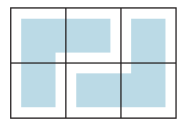
\includegraphics[scale=0.5]{../images/5.3.6.a.png}
\end{figure}
\end{proof}

\subsubsection{(b)}
Write $P(k)$.

\begin{proof}
$P(k)$ is the sentence “Any checkerboard with dimensions $2 \times 3k$ can be completely covered with L-shaped trominoes.”

\end{proof}

\subsubsection{(c)}
Write $P(k + 1)$.

\begin{proof}
$P(k + 1)$ is the sentence “Any checkerboard with dimensions $2 \times 3(k + 1)$ can be completely covered with L-shaped trominoes.”
\end{proof}

\subsubsection{(d)}
In a proof by mathematical induction that $P(n)$ is true for each integer $n \geq 1$, what must be shown in the inductive step?

\begin{proof}
The inductive step requires showing that for every integer $k \geq 1$, if any checkerboard with dimensions $2 \times 3k$ can be completely covered with L-shaped trominoes, then any checkerboard with dimensions $2 \times 3(k + 1)$ can be completely covered with L-shaped trominoes.
\end{proof}

\subsection{Exercise 7}
For each positive integer $n$, let $P(n)$ be the sentence:

In any round-robin tournament involving $n$ teams, the teams can be labeled $T_1, T_2, T_3, \ldots$, $T_n$, so that $T_i$ beats $T_{i + 1}$ for every $i = 1, 2, \ldots, n - 1$.

\subsubsection{(a)}
Write $P(2)$. Is $P(2)$ true?

\begin{proof}
$P(2)$ is the sentence ``In any round-robin tournament involving $2$ teams, the teams can be labeled $T_1, T_2$, so that $T_1$ beats $T_{2}$.'' It is true by Exercise 36 later.
\end{proof}

\subsubsection{(b)}
Write $P(k)$.

\begin{proof}
$P(k)$ is the sentence ``In any round-robin tournament involving $k$ teams, the teams can be labeled $T_1, T_2, T_3, \ldots$, $T_k$, so that $T_i$ beats $T_{i + 1}$ for every $i = 1, 2, \ldots, k$.''
\end{proof}

\subsubsection{(c)}
Write $P(k + 1)$.

\begin{proof}
$P(k + 1)$ is the sentence ``In any round-robin tournament involving $k + 1$ teams, the teams can be labeled $T_1, T_2, T_3, \ldots$, $T_{k + 1}$, so that $T_i$ beats $T_{i + 1}$ for every $i = 1, 2, \ldots, k + 1$.''
\end{proof}

\subsubsection{(d)}
In a proof by mathematical induction that $P(n)$ is true for each integer $n \geq 2$, what must be shown in the inductive step?

\begin{proof}
The inductive step requires showing that for every integer $k \geq 2$, if in any round-robin tournament involving $k$ teams, the teams can be labeled $T_1, T_2, T_3, \ldots$, $T_k$, so that $T_i$ beats $T_{i + 1}$ for every $i = 1, 2, \ldots, k$, then in any round-robin tournament involving $k + 1$ teams, the teams can be labeled $T_1, T_2, T_3, \ldots$, $T_{k + 1}$, so that $T_i$ beats $T_{i + 1}$ for every $i = 1, 2, \ldots, k + 1$.
\end{proof}

{\bf \cy Prove each statement in $8-23$ by mathematical induction.}

\subsection{Exercise 8}
$5^n - 1$ is divisible by 4, for every integer $n \geq 0$.

\begin{proof}
For the given statement, the property $P(n)$ is the sentence “$5^n - 1$ is divisible by 4.” 

{\bf Show that $P(0)$ is true:} 

$P(0)$ is the sentence “$5^0 - 1$ is divisible by 4.” Now $5^0 - 1 = 1 - 1 = 0$, and 0 is divisible by 4 because $0 = 4 \cdot 0$. Thus $P(0)$ is true. 

{\bf Show that for every integer $k \geq 0$, if $P(k)$ is true then $P(k + 1)$ is true:} 

Let $k$ be any integer with $k \geq 0$, and suppose $P(k)$ is true. That is, suppose $5^k - 1$ is divisible by 4. {\it [This is the inductive hypothesis.]} We must show that $P(k + 1)$ is true. That is, we must show that $5^{k + 1} - 1$ is divisible by 4. Now 

$5^{k + 1} - 1 = 5^k \cdot 5 - 1 = 5^k \cdot (4 + 1) - 1 = 5^k \cdot 4 + (5^k - 1)$. (*) 

By the inductive hypothesis, $5^k - 1$ is divisible by 4, and so $5^k - 1 = 4r$ for some integer $r$. Substitute $4r$ in place of $5^k - 1$ in equation (*), to obtain 

$5^{k + 1} - 1 = 5^k \cdot 4 + 4r = 4(5^k + r)$. 

But $5^k + r$ is an integer because $k$ and $r$ are integers. Hence, by definition of divisibility, $5^{k + 1} - 1$ is divisible by 4 {\it [as was to be shown]}. 

{\it An alternative proof of the inductive step goes as follows:} 

Let $k$ be any integer with $k \geq 0$, and suppose that $5^k - 1$ is divisible by 4. Then $5^k - 1 = 4r$ for some integer $r$, and hence $5^k = 4r + 1$. It follows that $5^{k + 1} = 5k \cdot 5 = (4r + 1) \cdot 5 = 20r + 5$. Subtracting 1 from both sides gives that $5^{k + 1} - 1 = 20r + 4 = 4(5r + 1)$. Now since $5r + 1$ is an integer, by definition of divisibility, $5^{k + 1} - 1$ is divisible by 4.
\end{proof}

\subsection{Exercise 9}
$7^n - 1$ is divisible by 6, for each integer $n \geq 0$.

\begin{proof}
For the given statement, the property $P(n)$ is the sentence “$7^n - 1$ is divisible by 6.” 

{\bf Show that $P(0)$ is true:} 

$P(0)$ is the sentence “$7^0 - 1$ is divisible by 6.” Now $7^0 - 1 = 1 - 1 = 0$, and 0 is divisible by 6 because $0 = 6 \cdot 0$. Thus $P(0)$ is true. 

{\bf Show that for every integer $k \geq 0$, if $P(k)$ is true then $P(k + 1)$ is true:} 

Let $k$ be any integer with $k \geq 0$, and suppose $P(k)$ is true. That is, suppose $7^k - 1$ is divisible by 6. {\it [This is the inductive hypothesis.]} We must show that $P(k + 1)$ is true. That is, we must show that $7^{k + 1} - 1$ is divisible by 6. Now 

$7^{k + 1} - 1 = 7^k \cdot 7 - 1 = 7^k \cdot (6 + 1) - 1 = 7^k \cdot 6 + (7^k - 1)$. (*) 

By the inductive hypothesis, $7^k - 1$ is divisible by 6, and so $7^k - 1 = 6r$ for some integer $r$. Substitute $6r$ in place of $7^k - 1$ in equation (*), to obtain 

$7^{k + 1} - 1 = 7^k \cdot 6 + 6r = 6(7^k + r)$. 

But $7^k + r$ is an integer because $k$ and $r$ are integers. Hence, by definition of divisibility, $7^{k + 1} - 1$ is divisible by 6 {\it [as was to be shown]}.
\end{proof}

\subsection{Exercise 10}
$n^3 - 7n + 3$ is divisible by 3, for each integer $n \geq 0$.

\begin{proof}
For the given statement, the property $P(n)$ is the sentence “$n^3 - 7n + 3$ is divisible by 3.” 

{\bf Show that $P(0)$ is true:} 

$P(0)$ is the sentence “$0^3 - 7 \cdot 0 + 3$ is divisible by 3.” Now $0^3 - 7 \cdot 0 + 3 = 3$, and 3 is divisible by 3 because $3 = 1 \cdot 3$. Thus $P(0)$ is true. 

{\bf Show that for every integer $k \geq 0$, if $P(k)$ is true then $P(k + 1)$ is true:} 

Let $k$ be any integer with $k \geq 0$, and suppose $P(k)$ is true. That is, suppose $k^3 - 7k + 3$ is divisible by 3. {\it [This is the inductive hypothesis.]} We must show that $P(k + 1)$ is true. That is, we must show that $(k+1)^3 - 7(k+1) + 3$ is divisible by 3. Now 

$(k+1)^3 - 7(k+1) + 3 = k^3 + 3k^2 + 3k + 1 - 7k - 7 + 3 = (k^3 - 7k + 3) + 3(k^2 + k - 2)$. (*) 

By the inductive hypothesis, $k^3 - 7k + 3$ is divisible by 3, and so $k^3 - 7k + 3 = 3r$ for some integer $r$. Substitute $3r$ in place of $k^3 - 7k + 3$ in equation (*), to obtain 

$(k+1)^3 - 7(k+1) + 3 = 3r + 3(k^2 + k - 2) = 3(r + k^2 + k - 2)$. 

But $r + k^2 + k - 2$ is an integer because $k$ and $r$ are integers. Hence, by definition of divisibility, $(k+1)^3 - 7(k+1) + 3$ is divisible by 3 {\it [as was to be shown]}.
\end{proof}

\subsection{Exercise 11}
$3^{2n} - 1$ is divisible by 8, for each integer $n \geq 0$.

\begin{proof}
For the given statement, the property $P(n)$ is the sentence “$3^{2n} - 1$ is divisible by 8.” 

{\bf Show that $P(0)$ is true:} 

$P(0)$ is the sentence “$3^{2 \cdot 0} - 1$ is divisible by 8.” Now $3^{2 \cdot 0} - 1 = 1 - 1 = 0$, and 0 is divisible by 8 because $0 = 8 \cdot 0$. Thus $P(0)$ is true. 

{\bf Show that for every integer $k \geq 0$, if $P(k)$ is true then $P(k + 1)$ is true:} 

Let $k$ be any integer with $k \geq 0$, and suppose $P(k)$ is true. That is, suppose $3^{2k} - 1$ is divisible by 8. {\it [This is the inductive hypothesis.]} We must show that $P(k + 1)$ is true. That is, we must show that $3^{2(k+1)} - 1$ is divisible by 8. Now 

$3^{2(k+1)} - 1 = 3^{2k+2} - 1 = 3^{2k} \cdot 3^2 - 1 = 3^{2k} \cdot 9 - 1 = 3^{2k} \cdot (8+1) - 1 = 3^{2k} \cdot 8 + 3^{2k} - 1$. (*) 

By the inductive hypothesis, $3^{2k} - 1$ is divisible by 8, and so $3^{2k} - 1 = 8r$ for some integer $r$. Substitute $8r$ in place of $3^{2k} - 1$ in equation (*), to obtain 

$3^{2(k+1)} - 1 = 3^{2k} \cdot 8 + 8r = 8(3^{2k} + r)$. 

But $3^{2k} + r$ is an integer because $k$ and $r$ are integers. Hence, by definition of divisibility, $3^{2(k+1)} - 1$ is divisible by 8 {\it [as was to be shown]}.
\end{proof}

\subsection{Exercise 12}
For any integer $n \geq 0$, $7^n - 2^n$ is divisible by 5.

\begin{proof}
For the given statement, the property $P(n)$ is the sentence “$7^n - 2^n$ is divisible by 5.” 

{\bf Show that $P(0)$ is true:} 

$P(0)$ is the sentence “$7^0 - 2^0$ is divisible by 5.” Now $7^0 - 2^0 = 1 - 1 = 0$, and 0 is divisible by 5 because $0 = 5 \cdot 0$. Thus $P(0)$ is true. 

{\bf Show that for every integer $k \geq 0$, if $P(k)$ is true then $P(k + 1)$ is true:} 

Let $k$ be any integer with $k \geq 0$, and suppose $P(k)$ is true. That is, suppose $7^k - 2^k$ is divisible by 5. {\it [This is the inductive hypothesis.]} We must show that $P(k + 1)$ is true. That is, we must show that $7^{k+1} - 2^{k+1}$ is divisible by 5. Now 

$7^{k+1} - 2^{k+1} = 7 \cdot 7^k - 2 \cdot 2^k = (5+2) \cdot 7^k - 2 \cdot 2^k = 5 \cdot 7^k + 2(7^k - 2^k)$. (*) 

By the inductive hypothesis, $7^k - 2^k$ is divisible by 5, and so $7^k - 2^k = 5r$ for some integer $r$. Substitute $5r$ in place of $7^k - 2^k$ in equation (*), to obtain 

$7^{k+1} - 2^{k+1} = 5 \cdot 7^k + 2(5r) = 5(7^k + 2r)$. 

But $7^k + 2r$ is an integer because $k$ and $r$ are integers. Hence, by definition of divisibility, $7^{k+1} - 2^{k+1}$ is divisible by 5 {\it [as was to be shown]}.
\end{proof}

\subsection{Exercise 13}
For any integer $n \geq 0, x^n - y^n$ is divisible by $x - y$, where $x$ and $y$ are any integers with $x \neq y$.

{\it Hint:} $x^{k+1} - y^{k+1} = x^{k+1} - xy^k + xy^k - y^{k+1} = x(x^k - y^k) + y^k(x-y)$.

\begin{proof}
For the given statement, the property $P(n)$ is the sentence “$x^n - y^n$ is divisible by $x - y$.” 

{\bf Show that $P(0)$ is true:} 

$P(0)$ is the sentence “$x^0 - y^0$ is divisible by $x - y$..” Now $x^0 - y^0 = 1 - 1 = 0$, and 0 is divisible by $x - y$ because $0 = (x-y) \cdot 0$. Thus $P(0)$ is true. 

{\bf Show that for every integer $k \geq 0$, if $P(k)$ is true then $P(k + 1)$ is true:} 

Let $k$ be any integer with $k \geq 0$, and suppose $P(k)$ is true. That is, suppose $x^k - y^k$ is divisible by $x-y$. {\it [This is the inductive hypothesis.]} We must show that $P(k + 1)$ is true. That is, we must show that $7^{k+1} - 2^{k+1}$ is divisible by $x-y$. Now 

$x^{k+1} - y^{k+1} = x^{k+1} - xy^k + xy^k - y^{k+1} = x(x^k - y^k) + y^k(x-y)$. (*) 

By the inductive hypothesis, $x^k - y^k$ is divisible by $x-y$, and so $x^k - y^k = (x-y)r$ for some integer $r$. Substitute $(x-y)r$ in place of $x^k - y^k$ in equation (*), to obtain 

$x^{k+1} - y^{k+1} = x(x - y)r + y^k(x-y) = (x-y)[xr + y^k]$. 

But $xr + y^k$ is an integer because $k, x, y$ and $r$ are integers. Hence, by definition of divisibility, $x^{k+1} - y^{k+1}$ is divisible by $x - y$ {\it [as was to be shown]}.
\end{proof}

\subsection{Exercise 14}
$n^3 - n$ is divisible by 6, for each integer $n \geq 0$.

{\it Hint 1:} $(k + 1)^3 - (k + 1) = k^3 + 3k^2 + 3k + 1 - k - 1 = (k^3 - k) + 3k^2 + 3k = (k^3 - k) + 3k(k + 1)$.

{\it Hint 2:} $k(k + 1)$ is a product of two consecutive integers. By Theorem 4.5.2, one of these must be even.

\begin{proof}
{\it Note:} It is possible to prove this without mathematical induction, because $n^3 - n = n(n^2 - 1) = n(n-1)(n+1)$ is the product of 3 consecutive integers. Therefore one of them is divisible by 3, and one of them is even, hence their product is divisible by 6.

For the given statement, the property $P(n)$ is the sentence “$n^3 - n$ is divisible by 6.” 

{\bf Show that $P(0)$ is true:} 

$P(0)$ is the sentence “$n^3 - n$ is divisible by 6.” Now $0^3 - 0 = 0 - 0 = 0$, and 0 is divisible by 6 because $0 = 6 \cdot 0$. Thus $P(0)$ is true. 

{\bf Show that for every integer $k \geq 0$, if $P(k)$ is true then $P(k + 1)$ is true:} 

Let $k$ be any integer with $k \geq 0$, and suppose $P(k)$ is true. That is, suppose $k^3 - k$ is divisible by 6. {\it [This is the inductive hypothesis.]} We must show that $P(k + 1)$ is true. That is, we must show that $(k+1)^3 - (k+1)$ is divisible by 6. Now 

$(k + 1)^3 - (k + 1) = k^3 + 3k^2 + 3k + 1 - k - 1 = (k^3 - k) + 3k(k + 1)$. (*)

By the inductive hypothesis, $k^3 - k$ is divisible by 6, and so $k^3 - k = 6r$ for some integer $r$. Moreover $k(k+1)$ is even by Theorem 4.5.2, so $k(k+1) = 2s$ for some integer $s$. Substitute $6r$ in place of $k^3 - k$ and $2s$ in place of $k(k+1)$ in equation (*), to obtain 

$(k + 1)^3 - (k + 1) = 6r + 3(2s) = 6r + 6s = 6(r+s)$.

But $r+s$ is an integer because $r$ and $s$ are integers. Hence, by definition of divisibility, $(k + 1)^3 - (k + 1)$ is divisible by 6 {\it [as was to be shown]}.
\end{proof}

\subsection{Exercise 15}
$n(n^2 + 5)$ is divisible by 6, for each integer $n \geq 0$.

\begin{proof}
For the given statement, the property $P(n)$ is the sentence “$n(n^2 + 5)$ is divisible by 6.” 

{\bf Show that $P(0)$ is true:} 

$P(0)$ is the sentence “$0(0^2 + 5)$ is divisible by 6.” Now $0(0^2 + 5) = 0$, and 0 is divisible by 6 because $0 = 6 \cdot 0$. Thus $P(0)$ is true. 

{\bf Show that for every integer $k \geq 0$, if $P(k)$ is true then $P(k + 1)$ is true:} 

Let $k$ be any integer with $k \geq 0$, and suppose $P(k)$ is true. That is, suppose $k(k^2 + 5)$ is divisible by 6. {\it [This is the inductive hypothesis.]} We must show that $P(k + 1)$ is true. That is, we must show that $(k+1)((k+1)^2 + 5)$ is divisible by 6. Now 

$(k+1)((k+1)^2 + 5) = (k+1)^3 + 5(k+1) = k^3 + 3k^2 + 3k + 1 + 5k + 5 =$

$= (k^3 + 5k) + (3k^2 + 3k + 6) = k(k^2 + 5) + 3(k^2 + k + 2) = k(k^2 + 5) + 3(k(k+1) + 2)$. (*)

By the inductive hypothesis, $k(k^2 + 5)$ is divisible by 6, and so $k(k^2 + 5) = 6r$ for some integer $r$. Moreover $k(k+1)$ is even by Theorem 4.5.2, so $k(k+1) = 2s$ for some integer $s$. Substitute $6r$ in place of $k(k^2 + 5)$ and $2s$ in place of $k(k+1)$ in equation (*), to obtain 

$(k+1)((k+1)^2 + 5) = 6r + 3(2s + 2) = 6r + 6s + 6 = 6(r + s + 1)$.

But $r + s + 1$ is an integer because $r$ and $s$ are integers. Hence, by definition of divisibility, $(k + 1)((k + 1)^2 + 5)$ is divisible by 6 {\it [as was to be shown]}.
\end{proof}

\subsection{Exercise 16}
$2^n < (n + 1)!$, for every integer $n \geq 2$.

\begin{proof}
For the given statement, the property $P(n)$ is the inequality $2^n < (n + 1)!$. 

{\bf Show that $P(2)$ is true:} 

$P(2)$ says that $2^2 < (2 + 1)!$. The left-hand side is $2^2 = 4$ and the right-hand side is $(2+1)! = 3! = 6$. So, because $4 < 6$, $P(2)$ is true. 

{\bf Show that for every integer $k \geq 2$, if $P(k)$ is true then $P(k + 1)$ is true:} 

Let $k$ be any integer with $k \geq 2$, and suppose $P(k)$ is true. That is, suppose $2^k < (k + 1)!$. {\it [This is the inductive hypothesis.]} We must show that $P(k + 1)$ is true. That is, we must show that $2^{k+1} < ((k+1) + 1)!$, or, equivalently, $2^{k+1} < (k + 2)!$. By the laws of exponents and the induction hypothesis,
\[
2^{k+1} = 2 \cdot 2^k < 2(k+1)!.
\]
Since $k \geq 2$, then $2 < k+2$, so
\[
2^{k+1} = 2 \cdot 2^k < 2(k+1)! < (k+2)(k+1)! = (k+2)!.
\]
So $2^{k+1} < (k+2)!$ {\it [as was to be shown]}.
\end{proof}

\subsection{Exercise 17}
$1 + 3n \leq 4^n$, for every integer $n \geq 0$.

\begin{proof}
For the given statement, the property $P(n)$ is the inequality $1 + 3n \leq 4^n$. 

{\bf Show that $P(0)$ is true:} 

$P(0)$ says that $1 + 3 \cdot 0 \leq 4^0$. The left-hand side is $1 + 3 \cdot 0 = 1$ and the right-hand side is $4^0 = 1$. So, because $1 \leq 1$, $P(0)$ is true. 

{\bf Show that for every integer $k \geq 0$, if $P(k)$ is true then $P(k + 1)$ is true:} 

Let $k$ be any integer with $k \geq 0$, and suppose $P(k)$ is true. That is, suppose $1 + 3k \leq 4^k$. {\it [This is the inductive hypothesis.]} We must show that $P(k + 1)$ is true. That is, we must show that $1 + 3(k+1) \leq 4^{k+1}$, or, equivalently, $1+3k+3 < 4 \cdot 4^k$. 

Now by the induction hypothesis, $1 + 3k + 3 \leq 4^k + 3$. So we need to show that $4^k + 3 \leq 4 \cdot 4^k$.

Since $0 \leq k$, we have $1 \leq 4^k$. So $3 \leq 3 \cdot 4^k$. Adding $4^k$ to both sides we get $3 + 4^k \leq 3 \cdot 4^k + 4^k = 4 \cdot 4^k$. Thus $3 + 4^k \leq 4 \cdot 4^k$.

So we have $1 + 3k + 3 \leq 4^k + 3$ and $3 + 4^k \leq 4 \cdot 4^k$. Combining these we get $1 + 3k + 3 \leq 4 \cdot 4^k$, in other words $1 + 3(k+1) \leq 4^{k+1}$, {\it [as was to be shown]}.
\end{proof}

\subsection{Exercise 18}
$5^n + 9 < 6^n$, for each integer $n \geq 2$.

\begin{proof}
For the given statement, the property $P(n)$ is the inequality $5^n + 9 < 6^n$. 

{\bf Show that $P(2)$ is true:} 

$P(2)$ says that $5^2 + 9 < 6^2$. The left-hand side is $5^2 + 9 = 25 + 9 = 34$ and the right-hand side is $6^2 = 36$. So, because $34 < 36$, $P(2)$ is true. 

{\bf Show that for every integer $k \geq 2$, if $P(k)$ is true then $P(k + 1)$ is true:} 

Let $k$ be any integer with $k \geq 2$, and suppose $P(k)$ is true. That is, suppose $5^k + 9 < 6^k$. {\it [This is the inductive hypothesis.]} We must show that $P(k + 1)$ is true. That is, we must show that $5^{k+1} + 9 < 6^{k+1}$. Now by laws of exponents and the induction hypothesis,
\[
5^{k+1} + 9 = 5 \cdot 5^k + 9 = (4 + 1) \cdot 5^k + 9 = 4 \cdot 5^k + (5^k + 9) < 4 \cdot 5^k + 6^k. (*)
\]
So we need to show $4 \cdot 5^k + 6^k < 6^{k+1}$.

Notice that since $4 < 5$ (and $5^k$ is positive) we have $4 \cdot 5^k < 5 \cdot 5^k$, and since $5 < 6$ (and $k \geq 2$) we have $5^k < 6^k$, and therefore $5 \cdot 5^k < 5 \cdot 6^k$. By transitivity of $<$, we get $4 \cdot 5^k < 5 \cdot 6^k$.

Since $4 \cdot 5^k < 5 \cdot 6^k$, adding $6^k$ to both sides we get $4 \cdot 5^k + 6^k < 5 \cdot 6^k + 6^k = 6 \cdot 6^k = 6^{k+1}$.

Combining this with (*) we get $5^{k+1} + 9 < 6^{k+1}$, {\it [as was to be shown]}.
\end{proof}

\subsection{Exercise 19}
$n^2 < 2^n$, for every integer $n \geq 5$.

\begin{proof}
For the given statement, the property $P(n)$ is the inequality $n^2 < 2^n$. 

{\bf Show that $P(5)$ is true:} 

$P(5)$ says that $5^2 < 2^5$. The left-hand side is $5^2 = 25$ and the right-hand side is $2^5 = 32$. So, because $25 < 32$, $P(5)$ is true. 

{\bf Show that for every integer $k \geq 5$, if $P(k)$ is true then $P(k + 1)$ is true:} 

Let $k$ be any integer with $k \geq 5$, and suppose $P(k)$ is true. That is, suppose $k^2 < 2^k$. {\it [This is the inductive hypothesis.]} We must show that $P(k + 1)$ is true. That is, we must show that $(k+1)^2 < 2^{k+1}$. 

Now by algebra and the induction hypothesis, $(k+1)^2 = k^2 + 2k + 1 < 2^k + 2k + 1$. Also by Proposition 5.3.2, $2k + 1 < 2^k$. Putting these inequalities together gives
\[
(k+1)^2 < 2^k + 2k + 1 < 2^k + 2^k = 2 \cdot 2^k = 2^{k+1}
\]
{\it [as was to be shown]}.
\end{proof}

\subsection{Exercise 20}
$2^n < (n + 2)!$, for each integer $n \geq 0$.

\begin{proof}
For the given statement, the property $P(n)$ is the inequality $n^2 < 2^n$. 

{\bf Show that $P(0)$ is true:} 

$P(0)$ says that $2^0 < (0 + 2)!$. The left-hand side is $2^0 = 1$ and the right-hand side is $(0 + 2)! = 2! = 2$. So, because $1 < 2$, $P(0)$ is true. 

{\bf Show that for every integer $k \geq 0$, if $P(k)$ is true then $P(k + 1)$ is true:} 

Let $k$ be any integer with $k \geq 0$, and suppose $P(k)$ is true. That is, suppose $2^k < (k + 2)!$. {\it [This is the inductive hypothesis.]} We must show that $P(k + 1)$ is true. That is, we must show that $2^{k+1} < (k + 3)!$. 

Now $2^{k+1} = 2 \cdot 2^k < 2 \cdot (k+2)!$ by the induction hypothesis. Since $k \geq 0$, we have $2 < k+3$, so $2 \cdot (k+2)! < (k+3) \cdot (k+2)! = (k+3)!$. Putting these two inequalities together gives $2^{k+1} < (k+3)!$, {\it [as was to be shown]}.
\end{proof}

\subsection{Exercise 21}
$\dps \sqrt{n} < \frac{1}{\sqrt{1}} + \frac{1}{\sqrt{2}} + \cdots + \frac{1}{\sqrt{n}}$, for every integer $n \geq 2$.

\begin{proof}
For the given statement, the property $P(n)$ is the inequality $\dps \sqrt{n} < \frac{1}{\sqrt{1}} + \frac{1}{\sqrt{2}} + \cdots + \frac{1}{\sqrt{n}}$. 

{\bf Show that $P(2)$ is true:} 

$P(2)$ says that $\dps \sqrt{2} < \frac{1}{\sqrt{1}} + \frac{1}{\sqrt{2}}$. The left-hand side is $\dps \sqrt{2} \approx 1.414$ and the right-hand side is $\dps \frac{1}{\sqrt{1}} + \frac{1}{\sqrt{2}} \approx 1 + \frac{1}{1.414} = 1.707$. So, because $1.414 < 1.707$, $P(2)$ is true. 

{\bf Show that for every integer $k \geq 2$, if $P(k)$ is true then $P(k + 1)$ is true:} 

Let $k$ be any integer with $k \geq 2$, and suppose $P(k)$ is true. That is, suppose $\dps \sqrt{k} < \frac{1}{\sqrt{1}} + \frac{1}{\sqrt{2}} + \cdots + \frac{1}{\sqrt{k}}$. {\it [This is the inductive hypothesis.]} We must show that $P(k + 1)$ is true. That is, we must show that $\dps \sqrt{k+1} < \frac{1}{\sqrt{1}} + \frac{1}{\sqrt{2}} + \cdots + \frac{1}{\sqrt{k+1}}$. 

Now the right-hand side of $P(k+1)$ is $\dps \frac{1}{\sqrt{1}} + \frac{1}{\sqrt{2}} + \cdots + \frac{1}{\sqrt{k+1}}$

\begin{center}
\begin{tabular}{lll}
= & $\dps \frac{1}{\sqrt{1}} + \frac{1}{\sqrt{2}} + \cdots + \frac{1}{\sqrt{k}} + \frac{1}{\sqrt{k+1}}$ & {\cy make next-to-last term explicit} \\
$>$ & $\dps \sqrt{k} + \frac{1}{\sqrt{k+1}}$ & {\cy by inductive hypothesis} \\
= & $\dps \sqrt{k} \cdot \frac{\sqrt{k + 1}}{\sqrt{k + 1}} + \frac{1}{\sqrt{k+1}}$ & {\cy because $\frac{\sqrt{k + 1}}{\sqrt{k + 1}} = 1$} \\
$>$ & $\dps \sqrt{k} \cdot \frac{\sqrt{k}}{\sqrt{k + 1}} + \frac{1}{\sqrt{k+1}}$ & {\cy because $k + 1 > k$} \\
= & $\dps \frac{k}{\sqrt{k + 1}} + \frac{1}{\sqrt{k+1}}$ & {\cy by algebra} \\
= & $\dps \frac{k+1}{\sqrt{k + 1}}$ & {\cy by adding fractions} \\
= & $\dps \sqrt{k + 1}$ & {\cy by canceling $\sqrt{k+1}$}
\end{tabular}
\end{center}

{\it [as was to be shown]}.
\end{proof}

\subsection{Exercise 22}
$1 + nx \leq (1 + x)^n$, for every real number $x > -1$
and every integer $n \geq 2$.

\begin{proof}
For the given statement, the property $P(n)$ is the statement ``$1 + nx \leq (1 + x)^n$, for every real number $x > -1$''. 

{\bf Show that $P(2)$ is true:} 

$P(2)$ says that $1 + 2x \leq (1 + x)^2$, for every real number $x > -1$. The left-hand side is $1 + 2x$ and the right-hand side is $(1+x)^2 = 1 + 2x + x^2$. So, because $0 \leq x^2$ for every real number $x > -1$, adding $1 + 2x$ to both sides gives us $1 + 2x \leq 1 + 2x + x^2$. So $P(2)$ is true. 

{\bf Show that for every integer $k \geq 2$, if $P(k)$ is true then $P(k + 1)$ is true:} 

Let $k$ be any integer with $k \geq 2$, and suppose $P(k)$ is true. That is, suppose $1 + kx \leq (1 + x)^k$, for every real number $x > -1$. {\it [This is the inductive hypothesis.]} We must show that $P(k + 1)$ is true. That is, we must show that $1 + (k + 1)x \leq (1 + x)^{k + 1}$, for every real number $x > -1$. 

Now the left-hand side of $P(k+1)$ is $1 + (k + 1)x = 1 + kx + x \leq (1 + x)^k + x$ by inductive hypothesis. 

We want to show $x \leq x(1+x)^k$. There are two cases:

{\bf Case 1: $-1 < x < 0$.} Then $0 < 1 + x < 1$, so $0 < (1+x)^k < 1$. So $0 > x(1+x)^k > x$ (since $x$ is negative).

{\bf Case 2: $0 \leq x$.} Then $1 \leq 1+x$, so $1 \leq (1 + x)^k$. Multiplying both sides by $x$ we get $x \leq x(1 + x)^k$ since $x$ is positive.

Combining the two inequalities $1 + (k + 1)x \leq (1 + x)^k + x$ and $x \leq x(1 + x)^k$ we get 
\[
1 + (k + 1)x \leq (1 + x)^k + x(1 + x)^k = (1 + x)^k (1 + x) = (1 + x)^{k + 1}
\]
{\it [as was to be shown]}.
\end{proof}

\subsection{Exercise 23}

\subsubsection{(a)}
$n^3 > 2n + 1$, for each integer $n \geq 2$.

\begin{proof}
For the given statement, the property $P(n)$ is the inequality $n^3 > 2n + 1$. 

{\bf Show that $P(2)$ is true:} 

$P(2)$ says that $2^3 > 2\cdot2 + 1$. The left-hand side is $2^3 = 8$ and the right-hand side is $2 \cdot 2 + 1 = 5$. So, because $8 > 5$, $P(2)$ is true. 

{\bf Show that for every integer $k \geq 2$, if $P(k)$ is true then $P(k + 1)$ is true:} 

Let $k$ be any integer with $k \geq 2$, and suppose $P(k)$ is true. That is, suppose $k^3 > 2k + 1$. {\it [This is the inductive hypothesis.]} We must show that $P(k + 1)$ is true. That is, we must show that $(k + 1)^3 > 2(k + 1) + 1$. 

Now $(k + 1)^3 = k^3 + 3k^2 + 3k + 1 > (2k + 1) + 3k^2 + 3k + 1$ by the induction hypothesis. Since $k \geq 2$, we have $3k^2 + 3k \geq 3 \cdot 2^2 + 3 \cdot 2 = 18 > 2$, so
\[
(k + 1)^3 > (2k + 1) + 3k^2 + 3k + 1 > 2k + 1 + 2 = 2k + 3 = 2(k + 1) + 1
\]
{\it [as was to be shown]}.
\end{proof}

\subsubsection{(b)}
$n! > n^2$, for each integer $n \geq 4$.

\begin{proof}
For the given statement, the property $P(n)$ is the inequality $n! > n^2$. 

{\bf Show that $P(4)$ is true:} 

$P(4)$ says that $4! > 4^2$. The left-hand side is $4! = 24$ and the right-hand side is $4^2 = 16$. So, because $24 > 16$, $P(4)$ is true. 

{\bf Show that for every integer $k \geq 4$, if $P(k)$ is true then $P(k + 1)$ is true:} 

Let $k$ be any integer with $k \geq 4$, and suppose $P(k)$ is true. That is, suppose $k! > k^2$. {\it [This is the inductive hypothesis.]} We must show that $P(k + 1)$ is true. That is, we must show that $(k + 1)! > (k + 1)^2$. 

We have $(k + 1)! = (k + 1) \cdot k! > (k + 1) \cdot k^2$ by the induction hypothesis. So we need to show $(k + 1) \cdot k^2 > (k + 1)^2$, or, equivalently, $k^2 > k+1$, or equivalently $k^2 - k - 1 > 0$.

From analytic geometry, we know that the roots of the equation $k^2 - k - 1 = 0$ are $k = \dps \frac{-(-1) \pm \sqrt{(-1)^2 - 4(1)(-1)}}{2(1)} = \frac{1 \pm \sqrt{5}}{2} \approx 0.618$ and $1.618$. Since the leading coefficient of the quadratic polynomial $k^2 - k - 1$ is positive, it has a U-shape and it's positive for all values of $k$ greater than the larger root 1.618. Since $k \geq 4$ it follows that $k^2 - k - 1 > 0$.
\end{proof}

\subsection{Exercise 24}
A sequence $a_1, a_2, a_3, \ldots$ is defined by letting $a_1 = 3$ and $a_k = 7a_{k-1}$ for each integer $k \geq 2$. Show that $a_n = 3\cdot 7^n - 1$ for every integer $n \geq 1$.

\begin{proof}
For the given statement, the property $P(n)$ is the equation $a_n = 3 \cdot 7^{n - 1}$. 

{\bf Show that $P(1)$ is true:} 

The left-hand side is $a_1$, which equals 3 by the definition of the sequence. The right-hand side is $4 \cdot 7^{1 - 1} = 3$ also. Thus $P(1)$ is true. 

{\bf Show that for every integer $k \geq 1$, if $P(k)$ is true then $P(k + 1)$ is true:} 

Let $k$ be any integer with $k \geq 1$, and suppose $P(k)$ is true. That is, suppose $a_k = 3 \cdot 7^{k - 1}$. {\it [This is the inductive hypothesis.]} We must show that $P(k + 1)$ is true. That is, we must show that $a_{k + 1} = 3 \cdot 7^{(k + 1) - 1}$, or, equivalently, $a_{k + 1} = 3 \cdot 7^k$. But the left-hand side of $P(k+1)$ is $a_{k+1}$

\begin{center}
\begin{tabular}{rlll}
$a_{k+1}$ & = & $7a_k$ & {\cy by definition of the sequence} \\
& = & $7(3 \cdot 7^{k - 1})$ & {\cy by inductive hypothesis} \\
& = & $3 \cdot 7^k$ & {\cy by laws of exponents} \\
\end{tabular}
\end{center}

which is the right-hand side of $P(k + 1)$, {\it [as was to be shown]}.
\end{proof}

\subsection{Exercise 25}
A sequence $b_0, b_1, b_2, \ldots$ is defined by letting
$b_0 = 5$ and $b_k = 4 + b_{k-1}$ for each integer $k \geq 1$. Show that $b_n > 4n$ for every integer $n \geq 0$.

\begin{proof}
Let the property $P(n)$ be the inequality $b_n > 4n$. 

{\bf Show that $P(0)$ is true:} 

The left-hand side is $b_0$, which equals 5 by the definition of the sequence. The right-hand side is $4 \cdot 0 = 0$ and $5 > 0$. Thus $P(0)$ is true. 

{\bf Show that for every integer $k \geq 0$, if $P(k)$ is true then $P(k + 1)$ is true:} 

Let $k$ be any integer with $k \geq 0$, and suppose that $b_k > 4k$ ({\cy inductive hypothesis}). We must show that $b_{k + 1} > 4(k+1)$. Now

\begin{center}
\begin{tabular}{rlll}
$b_{k+1}$ & = & $4 + b_k$ & {\cy by definition of the sequence} \\
& $>$ & $4 + 4k$ & {\cy by inductive hypothesis} \\
& = & $4(1 + k)$ & {\cy by factoring out a 4} \\
& = & $4(k + 1)$ & {\cy by commutative law for addition}
\end{tabular}
\end{center}

{\it [as was to be shown]}.
\end{proof}

\subsection{Exercise 26}
A sequence $c_0, c_1, c_2, \ldots$ is defined by letting
$c_0 = 3$ and $c_k = (c_{k-1})^2$ for every integer $k \geq 1$. Show that $\dps c_n = 3^{2^n}$ for each integer $n \geq 0$.

\begin{proof}
Let the property $P(n)$ be the equation $\dps c_n = 3^{2^n}$. 

{\bf Show that $P(0)$ is true:} 

The left-hand side is $c_0$, which equals 3 by the definition of the sequence. The right-hand side is $\dps 3^{2^0} = 3^1 = 3$ and $3 = 3$. Thus $P(0)$ is true. 

{\bf Show that for every integer $k \geq 0$, if $P(k)$ is true then $P(k + 1)$ is true:} 

Let $k$ be any integer with $k \geq 0$, and suppose that $\dps c_k = 3^{2^k}$ ({\cy inductive hypothesis}). We must show that $c_{k + 1} = 3^{2^{k+1}}$. Now

\begin{center}
\begin{tabular}{rlll}
$c_{k+1}$ & = & $(c_k)^2$ & {\cy by definition of the sequence} \\
& = & $\dps (3^{2^k})^2$ & {\cy by inductive hypothesis} \\
& = & $3^{2^k \cdot 2}$ & {\cy by laws of exponents} \\
& = & $3^{2^{k + 1}}$ & {\cy by laws of exponents}
\end{tabular}
\end{center}

{\it [as was to be shown]}.
\end{proof}

\subsection{Exercise 27}
A sequence $d_1, d_2, d_3, \ldots$ is defined by letting $d_1 = 2$ and $\dps d_k = \frac{d_{k-1}}{k}$ for each integer $k \geq 2$. Show that for every integer $\dps n \geq 1, d_n = \frac{2}{n!}$. 

\begin{proof}
Let the property $P(n)$ be the equation $\dps d_n = \frac{2}{n!}$. 

{\bf Show that $P(1)$ is true:} 

The left-hand side is $d_1$, which equals 2 by the definition of the sequence. The right-hand side is $\dps \frac{2}{1!} = 2$ and $2 = 2$. Thus $P(1)$ is true. 

{\bf Show that for every integer $k \geq 1$, if $P(k)$ is true then $P(k + 1)$ is true:} 

Let $k$ be any integer with $k \geq 1$, and suppose that $\dps d_k = \frac{2}{k!}$ ({\cy inductive hypothesis}). We must show that $\dps d_{k + 1} = \frac{2}{(k + 1)!}$. Now

\begin{center}
\begin{tabular}{rlll}
\vspace{0.3cm}
$d_{k+1}$ & = & $\dps \frac{d_k}{k+1}$ & {\cy by definition of the sequence} \\
\vspace{0.3cm}
& = & $\dps \frac{\frac{2}{k!}}{k+1}$ & {\cy by inductive hypothesis} \\
& = & $\dps \frac{2}{k!(k+1)}$ & {\cy by algebra} \\
& = & $\dps \frac{2}{(k + 1)!}$ & {\cy by definition of !}
\end{tabular}
\end{center}

{\it [as was to be shown]}.
\end{proof}

\subsection{Exercise 28}
Prove that for every integer $n \geq 1$,
\[
\frac{1}{3} = \frac{1 + 3 + 5 + \cdots + (2n-1)}{(2n+1) + (2n+3) + \cdots + (2n + (2n-1))}
\]
\begin{proof}
Let the property $P(n)$ be the equation 

\[
\dps \frac{1}{3} = \frac{1 + 3 + 5 + \cdots + (2n-1)}{(2n+1) + (2n+3) + \cdots + (2n + (2n-1))}.
\] 

{\bf Show that $P(1)$ is true:} 

The left-hand side is $1/3$. The right-hand side is $\dps \frac{1}{(2 \cdot 1 + 1)} = 1/3$ also. Thus $P(1)$ is true. 

{\bf Show that for every integer $k \geq 1$, if $P(k)$ is true then $P(k + 1)$ is true:} 

Let $k$ be any integer with $k \geq 1$, and suppose that 
\[
\dps \frac{1}{3} = \frac{1 + 3 + 5 + \cdots + (2k-1)}{(2k+1) + (2k+3) + \cdots + (2k + (2k-1))}
\]
({\cy inductive hypothesis}). We must show that 
\[
\dps \frac{1}{3} = \frac{1 + 3 + 5 + \cdots + (2(k+1)-1)}{(2(k+1)+1) + (2(k+1)+3) + \cdots + (2(k+1) + (2(k+1)-1))}.\] 
Now from the inductive hypothesis, we get by cross-multiplying:
\[
(2k+1) + (2k+3) + \cdots + (2k + (2k-1)) = 3[1 + 3 + 5 + \cdots + (2k-1)]
\]
For each term on the left-hand side, we add 2 to both sides. This way, $(2k + 1)$ becomes $(2k + 1) + 2 = (2(k+1) + 1)$, $(2k + 3)$ becomes $(2k + 3) + 2 = (2(k+1) + 3)$, and so on. There are $(2k - 1 + 1) / 2 = k$ terms on the left-hand side, therefore we are adding a total of $2k$ to both sides. We get:
\[
(2(k+1)+1) + (2(k+1)+3) + \cdots + (2(k+1) + (2k-1)) = 3[1 + 3 + 5 + \cdots + (2k-1)] + 2k
\]
Now add the last missing term $(2(k+1) + (2(k+1)-1))$ to both sides:

$(2(k+1)+1) + (2(k+1)+3) + \cdots + (2(k+1) + (2k-1)) + (2(k+1) + (2(k+1)-1))$

$ = 3[1 + 3 + 5 + \cdots + (2k-1)] + 2k + (2(k+1) + (2(k+1)-1))$

Notice that $2k + (2(k+1) + (2(k+1)-1)) = 6k + 3 = 3(2k+1) = 3(2(k+1) - 1)$. Therefore

$(2(k+1)+1) + (2(k+1)+3) + \cdots + (2(k+1) + (2k-1)) + (2(k+1) + (2(k+1)-1))$

$ = 3[1 + 3 + 5 + \cdots + (2k-1) + (2(k+1)-1)]$.

Dividing both sides by (3 times the left-hand side), we get:
\[
\dps \frac{1}{3} = \frac{1 + 3 + 5 + \cdots + (2(k+1)-1)}{(2(k+1)+1) + (2(k+1)+3) + \cdots + (2(k+1) + (2(k+1)-1))}\] 
{\it [as was to be shown]}.
\end{proof}

{\bf \cy Exercises 29 and 30 use the definition of string and string length from page 13 in Section 1.4. Recursive definitions for these terms are given in Section 5.9.}

\subsection{Exercise 29}
A set $L$ consists of strings obtained by juxtaposing one or more of $abb, bab$, and $bba$. Use mathematical induction to prove that for every integer $n \geq 1$, if a string $s$ in $L$ has length $3n$, then $s$ contains an even number of $b$’s.

\begin{proof}
Let the property $P(n)$ be the sentence “If a string $s$ in $L$ has length $3n$, then $s$ contains an even number of $b$’s.” 

{\bf Show that $P(1)$ is true:} $P(1)$ is the statement that a string $s$ in $L$ of length 3 contains an even number of $b$’s. The only strings in $L$ that have length 3 are $abb, bab$, and $bba$, and each of these strings has an even number of $b$’s. So $P(1)$ is true.

{\bf Show that for every integer $k \geq 1$, if $P(k)$ is true then $P(k + 1)$ is true:} Let $k$ be any integer with $k \geq 1$ and suppose that if a string $s$ in $L$ has length $3k$, then $s$ contains an even number of $b$’s. {\cy $\from P(k)$ inductive hypothesis}

We must show that if a string $s$ in $L$ has length $3(k + 1)$, then $s$ contains an even number of $b$’s. {\cy $\from P(k + 1)$} 

So, suppose $s$ is a string in $L$ that has length $3(k + 1)$. Now $3(k + 1) = 3k + 3$ and the strings in $L$ are obtained by juxtaposing strings already in $L$ with one of $abb, bab$, or $bba$. Thus, either the initial or the final three characters in $s$ are $abb$, $bab$, or $bba$. Moreover, the other $3k$ characters in $s$ are also in $L$ by definition of $L$, and so, by inductive hypothesis, the other $3k$ characters in $s$ contain an even number, say $m$, of $b$’s. Because each of $abb$, $bab$, and $bba$ contains 2 $b$’s, the total number of $b$’s in $s$ is $m + 2$, which is a sum of even integers and hence is even {\it [as was to be shown]}. 
\end{proof}

\subsection{Exercise 30}
A set $S$ consists of strings obtained by juxtaposing one or more copies of 1110 and 0111. Use mathematical induction to prove that for every integer $n \geq 1$, if a string $s$ in $S$ has length $4n$, then the number of 1’s in $s$ is a multiple of 3.

\begin{proof}
Let the property $P(n)$ be the sentence “If a string $s$ in $S$ has length $4n$, then the number of 1’s in $s$ is a multiple of 3.” 

{\bf Show that $P(1)$ is true:} $P(1)$ is the statement that a string $s$ in $S$ of length 4 contains zero or three  1’s. The only strings in $S$ that have length 4 are 1110 and 0111, and each of these strings has three 1’s. So $P(1)$ is true.

{\bf Show that for every integer $k \geq 1$, if $P(k)$ is true then $P(k + 1)$ is true:} Let $k$ be any integer with $k \geq 1$ and suppose that if a string $s$ in $S$ has length $4k$, then the number of 1’s in $s$ is a multiple of 3. {\cy $\from P(k)$ inductive hypothesis}

We must show that if a string $s$ in $S$ has length $4(k + 1)$, then the number of 1’s in $s$ is a multiple of 3. {\cy $\from P(k + 1)$} 

So, suppose $s$ is a string in $S$ that has length $4(k + 1)$. Now $4(k + 1) = 4k + 4$ and the strings in $S$ are obtained by juxtaposing strings already in $S$ with one of 1110 or 0111. Thus, either the initial or the final four characters in $s$ are 1110 or 0111. Moreover, the other $4k$ characters in $s$ are also in $S$ by definition of $S$, and so, by inductive hypothesis, the other $4k$ characters in $s$ contain a number of 1's divisible by 3, say $3m$ 1’s. Because each of 1110 and 0111 contains three 1’s, the total number of 1’s in $s$ is $3m + 3 = 3(m+1)$, which is a multiple of 3 {\it [as was to be shown]}. 
\end{proof}

\subsection{Exercise 31}
Use mathematical induction to give an alternative proof for the statement proved in Example 4.9.9: For any positive integer $n$, a complete graph on $n$ vertices has $\frac{n(n - 1)}{2}$ edges. 

{\it Hint:} Let $P(n)$ be the sentence, ``the number of edges in a complete graph on $n$ vertices is $\frac{n(n - 1)}{2}$.''

\begin{proof}
Let $P(n)$ be as in the Hint above.

{\bf Show that $P(1)$ is true:} A complete graph on 1 vertex has no edges, and $\frac{1(1 - 1)}{2} = 0$, so $P(1)$ is true.

{\bf Show that for any integer $k \geq 1$ if $P(k)$ is true then $P(k+1)$ is true:}

Let $k$ be any integer with $k \geq 1$ and suppose that a complete graph on $k$ vertices has $\frac{k(k - 1)}{2}$ edges. {\cy $\from P(k)$ inductive hypothesis}

We must show that a complete graph on $k + 1$ vertices has $\frac{(k+1)k}{2}$ edges. {\cy $\from P(k + 1)$}

Let $K_{k+1}$ be a complete graph on $k+1$ vertices labeled $v_1, \ldots, v_k, v_{k+1}$. Consider the subgraph $K_k$ of $K_{k + 1}$ which is a complete graph on the first $k$ vertices $v_1, \ldots, v_k$.

Then the edges of $K_{k+1}$ can be divided into two disjoint sets: the edges of $K_k$, and the edges between $v_{k+1}$ and all the other edges $v_1, \ldots, v_k$.

By the inductive hypothesis the first set has $\frac{k(k-1)}{2}$ edges. Since $K_{k+1}$ is complete, the second set has $k$ additional edges (one edge between $v_{k + 1}$ and each one of $v_1, \ldots, v_k$).

Therefore the total number of edges of $K_{k+1}$ is the total of the two sets: $\frac{k(k-1)}{2} + k = \frac{k^2 - k + 2k}{2} = \frac{k^2 + k}{2} = \frac{(k+1)k}{2}$, {\it [as was to be shown.]}
\end{proof}

\subsection{Exercise 32}
Some $5 \times 5$ checkerboards with one square removed can be completely covered by L-shaped trominoes, whereas other $5 \times 5$ checkerboards cannot. Find examples of both kinds of checkerboards. Justify your answers.

{\it Hint:} Consider the problem of trying to cover a $3 \times 3$ checkerboard with trominoes. Place a checkmark in
certain squares as shown in the following figure.

\begin{center}
\begin{tabular}{|c|c|c|}
\hline
\checkmark & \hspace{0.4cm} & \checkmark \\
\hline
 & \hspace{0.4cm} & \\
\hline
\checkmark & \hspace{0.4cm} & \checkmark \\
\hline
\end{tabular}
\end{center}

Observe that no two squares containing checkmarks can be covered by the same tromino. Since there are four checkmarks, four trominoes would be needed to cover these squares. But, since each tromino covers three squares, four trominoes would cover twelve squares, not the nine squares in this checkerboard. It follows that such a covering is impossible.

\begin{proof}
For example, if we remove the center square, then the $5 \times 5$ board can be covered by L-shaped trominoes:

\begin{center}
\begin{tabular}{|c|c|c|c|c|}
\hline
\colsq{red} & \colsq{red} & \colsq{blue} & \colsq{green} & \colsq{green} \\
\hline
\colsq{red} & \colsq{blue} & \colsq{blue} & \colsq{magenta} & \colsq{green} \\
\hline
\colsq{brown} & \colsq{brown} &  & \colsq{magenta} & \colsq{magenta} \\
\hline
\colsq{brown} & \colsq{gray} & \colsq{cyan} & $\blacksquare$ & $\blacksquare$ \\
\hline
\colsq{gray} & \colsq{gray} & \colsq{cyan} & \colsq{cyan} & $\blacksquare$ \\
\hline
\end{tabular}
\end{center}

There are many other ways to remove 1 square from the 25, to make it work. The above is not the only one.

(Following the Hint) All 25 squares cannot be completely covered by L-shaped trominoes:

\begin{center}
\begin{tabular}{|c|c|c|c|c|}
\hline
\checkmark & \hspace{0.4cm} & \checkmark & \hspace{0.4cm} & \checkmark \\
\hline
 & \hspace{0.4cm} &  & \hspace{0.4cm} & \\
\hline
\checkmark & \hspace{0.4cm} & \checkmark & \hspace{0.4cm} & \checkmark \\
\hline
 & \hspace{0.4cm} &  & \hspace{0.4cm} & \\
\hline
\checkmark & \hspace{0.4cm} & \checkmark & \hspace{0.4cm} & \checkmark \\
\hline
\end{tabular}
\end{center}
\end{proof}

No two squares with checkmarks can be covered by the same L-shaped tromino. Since there are 9 checkmarks, we would need at least 9 trominoes, which cover 27 squares, exceeding the 25 squares. Therefore such a covering is impossible.

\subsection{Exercise 33}
Consider a $4 \times 6$ checkerboard. Draw a covering of the board by L-shaped trominoes.

\begin{proof}
\begin{center}
\begin{tabular}{|c|c|c|c|c|c|}
\hline
\colsq{red} & \colsq{red} & \colsq{blue} & \colsq{green} & \colsq{green} & \colsq{magenta} \\
\hline
\colsq{red} & \colsq{blue} & \colsq{blue} & \colsq{green} & \colsq{magenta} & \colsq{magenta} \\
\hline
\colsq{brown} & \colsq{brown} & \colsq{gray} & $\blacksquare$ & \colsq{yellow} & \colsq{yellow} \\
\hline
\colsq{brown} & \colsq{gray} & \colsq{gray} & $\blacksquare$ & $\blacksquare$ & \colsq{yellow} \\
\hline
\end{tabular}
\end{center}
\end{proof}

\subsection{Exercise 34}
\subsubsection{(a)}
Use mathematical induction to prove that for each integer $n \geq 1$, any checkerboard with dimensions $2 \times 3n$ can be completely covered with L-shaped trominoes.

{\it Hint:} For the inductive step, note that a $2 \times 3(k + 1)$ checkerboard can be split into a $2 \times 3k$ checkerboard and a $2 \times 3$ checkerboard.

\begin{proof}
Let the property $P(n)$ be ``any checkerboard with dimensions $2 \times 3n$ can be completely covered with L-shaped trominoes.''

{\bf Show that $P(1)$ is true:} $P(1)$ says ``A checkerboard with dimensions $2 \times 3$ can be completely covered with L-shaped trominoes.'' This is true:
\begin{tabular}{|c|c|c|}
\hline
\colsq{cyan} & \colsq{cyan} & \colsq{red} \\
\hline
\colsq{cyan} & \colsq{red} & \colsq{red} \\
\hline
\end{tabular}

{\bf Show that for any integer $k \geq 1$ if $P(k)$ is true then $P(k+1)$ is true:} Suppose $k$ is any integer with $k \geq 1$ such that $P(k)$ is true. That is, any checkerboard with dimensions $2 \times 3k$ can be completely covered with L-shaped trominoes. We want to show $P(k+1)$, that is, we want to show that any checkerboard with dimensions $2 \times 3(k+1)$ can be completely covered with L-shaped trominoes.

Consider any checkerboard with dimensions $2 \times 3(k+1)$, in other words with dimensions $2 \times (3k+3)$. This board can be split into two parts: a $2 \times 3k$ board on the left, and a $2 \times 3$ board on the right:
\begin{tabular}{|c|c|c|c|c|}
\hline
 &  &  & $\ldots$ &  \\
\hline
 &  &  & $\ldots$ &  \\
\hline
\end{tabular}
\hspace{0.5cm}
\begin{tabular}{|c|c|c|}
\hline
 &  &  \\
\hline
 &  &  \\
\hline
\end{tabular}

By the inductive hypothesis, the left part with dimensions $2 \times 3k$ can be completely covered with L-shaped trominoes. By $P(1)$, the right part with dimensions $2 \times 3$ can be completely covered with L-shaped trominoes. Putting these two coverings together we see that the whole board with dimensions $2 \times 3(k+1)$ can be completely covered with L-shaped trominoes, {\it [as was to be shown.]}
\end{proof}

\subsubsection{(b)}
Let $n$ be any integer greater than or equal to 1. Use the result of part (a) to prove by mathematical induction that for every integer $m \geq 1$, any checkerboard with dimensions $2m \times 3n$ can be completely covered with L-shaped trominoes.

\begin{proof}
Let the property $Q(m)$ be ``any checkerboard with dimensions $2m \times 3n$ can be completely covered with L-shaped trominoes.''

{\bf Show that $Q(1)$ is true:} $Q(1)$ says ``A checkerboard with dimensions $2 \times 3n$ can be completely covered with L-shaped trominoes.'' This is true by part (a).

{\bf Show that for any integer $k \geq 1$ if $Q(k)$ is true then $Q(k+1)$ is true:} Suppose $k$ is any integer with $k \geq 1$ such that $Q(k)$ is true. That is, any checkerboard with dimensions $2k \times 3n$ can be completely covered with L-shaped trominoes. We want to show $Q(k+1)$, that is, we want to show that any checkerboard with dimensions $2(k+1) \times 3n$ can be completely covered with L-shaped trominoes.

Consider any checkerboard with dimensions $2(k+1) \times 3n$, in other words with dimensions $(2k+2) \times 3n$. This board can be split into two parts: a $2k \times 3n$ board on the top, and a $2 \times 3n$ board on the bottom:

\begin{center}
\begin{tabular}{|c|c|c|c|c|}
\hline
 &  &  & $\ldots$ &  \\
\hline
 &  &  & $\ldots$ &  \\
\hline
 & $\vdots$ &  &  &  \\
\hline
 &  &  & $\ldots$ &  \\
\hline
\end{tabular}

\begin{tabular}{|c|c|c|c|c|}
\hline
 &  &  & $\ldots$ &  \\
\hline
 &  &  & $\ldots$ &  \\
\hline
\end{tabular}
\end{center}

By the inductive hypothesis, the top part with dimensions $2k \times 3n$ can be completely covered with L-shaped trominoes. By $Q(1)$, the bottom part with dimensions $2 \times 3n$ can be completely covered with L-shaped trominoes. Putting these two coverings together we see that the whole board with dimensions $2(k+1) \times 3n$ can be completely covered with L-shaped trominoes, {\it [as was to be shown.]}
\end{proof}

\subsection{Exercise 35}
Let $m$ and $n$ be any integers that are greater than or equal to 1.

\subsubsection{(a)}
Prove that a necessary condition for an $m \times n$ checkerboard to be completely coverable by L-shaped trominoes is that $mn$ be divisible by 3.

\begin{proof}
Assume an $m \times n$ checkerboard is completely coverable by L-shaped trominoes. {\it [We want to show that $mn$ is divisible by 3.]}

Since the board is coverable by L-shaped trominoes, there exists an integer $k \geq 1$ such that the board is covered with $k$ L-shaped trominoes. Since each tromino has 3 squares, and the trominoes do not overlap, the total number of squares covered by the covering is $3k$. 

Since the trominoes cover the whole board, and since the whole board has $mn$ squares, $mn = 3k$. So by definition of divisibility, $mn$ is divisible by 3.
\end{proof}

\subsubsection{(b)}
Prove that having $mn$ be divisible by 3 is not a sufficient condition for an $m \times n$ checkerboard to be completely coverable by L-shaped trominoes.

{\it Hint:} Consider a $3 \times 5$ checkerboard, and refer to the hint for Exercise 32. Figure out a way to place six checkmarks in squares so that no two of the squares that contain checkmarks can be covered by the same tromino.

\begin{proof}
(following the Hint)

Consider the $3 \times 5$ checkerboard below:

\begin{center}
\begin{tabular}{|c|c|c|c|c|}
\hline
\checkmark & \hspace{0.4cm} & \checkmark & \hspace{0.4cm} & \checkmark \\
\hline
 & \hspace{0.4cm} &  & \hspace{0.4cm} & \\
\hline
\checkmark & \hspace{0.4cm} & \checkmark & \hspace{0.4cm} & \checkmark \\
\hline
\end{tabular}
\end{center}

No L-shaped tromino can cover two of the checkmarked squares. So we need at least 6 trominoes to cover the checkmarked squares. However this gives us $6 \cdot 3 = 18$ squares, exceeding the 15 squares of the board. Therefore this covering is impossible.

Let $m = 5, n = 3$. Since $3 \cdot 5 = 15$ is divisible by 3 and the board is not coverable by L-shaped trominoes, we conclude that having $mn$ be divisible by 3 is not a sufficient condition for the $m \times n$ board to be coverable by L-shaped trominoes.
\end{proof}

\subsection{Exercise 36}
In a round-robin tournament each team plays every other team exactly once with ties not allowed. If the teams are labeled $T_1, T_2, \ldots, T_n$, then the outcome of such a tournament can be represented by a directed graph, in which the teams are represented as dots and an arrow is drawn from one dot to another if, and only if, the following team represented by the first dot beats the team represented by the second dot. For example, the following directed graph shows one outcome of a round-robin tournament involving five teams, A, B, C, D, and E.

\begin{figure}[ht!]
\centering
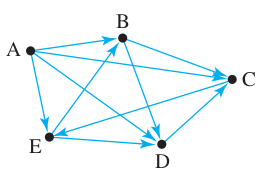
\includegraphics[scale=0.5]{../images/5.3.36.png}
\end{figure}

Use mathematical induction to show that in any round-robin tournament involving $n$ teams, where $n \geq 2$, it is possible to label the teams $T_1, T_2, \ldots, T_n$ so that $T_i$ beats $T_{i + 1}$ for all $i = 1, 2, \ldots, n - 1$. (For instance, one such labeling in the example above is $T_1 = A, T_2 = B, T_3 = C, T_4 = E, T_5 = D$.) ({\it Hint:} Given $k+1$ teams, pick one, say $T'$, and apply the inductive hypothesis to the remaining teams to obtain an ordering $T_1, T_2, \ldots, T_k$. Consider three cases: $T'$ beats $T_1$, $T'$ loses to the first $m$ teams (where $1 \leq m \leq k - 1$) and beats the $(m + 1)$st team, and $T'$ loses to all the other teams.)

\begin{proof}
Let the property $P(n)$ be ``in any round-robin tournament involving $n$ teams, it is possible to label the teams $T_1, T_2, \ldots, T_n$ so that $T_i$ beats $T_{i + 1}$ for all $i = 1, 2, \ldots, n - 1$.''.

{\bf Show that $P(2)$ is true:} In a round-robin tournament with two teams $A, B$, either $A$ beats $B$, in which case label $T_1 = A$ and $T_2 = B$, or $B$ beats $A$, in which case label $T_1 = B$ and $T_2 = A$. So in both cases $T_1$ beats $T_2$. So $P(2)$ is true.

{\bf Show that for every integer $k \geq 2$, if $P(k)$ is true then $P(k+1)$ is true:} Suppose $k \geq 2$ is any integer such that $P(k)$ is true. So in any round-robin tournament involving $k$ teams, it is possible to label the teams $T_1, T_2, \ldots, T_k$ so that $T_i$ beats $T_{i + 1}$ for all $i = 1, 2, \ldots, k - 1$. {\cy $\from P(k)$ inductive hypothesis}

{\it [We want to show that in any round-robin tournament involving $k+1$ teams, it is possible to label the teams $S_1, S_2, \ldots, S_{k+1}$ so that $S_i$ beats $S_{i + 1}$ for all $i = 1, 2, \ldots, k$.]} {\cy $\from P(k+1)$}

Given $k+1$ teams, pick one, say $X$. By the inductive hypothesis applied to the remaining $k$ teams, there exists an ordering $T_1, T_2, \ldots, T_k$ so that $T_i$ beats $T_{i + 1}$ for all $i = 1, 2, \ldots, k - 1$.

{\bf Case 1: $X$ beats $T_1$.} Then label the $k+1$ teams as follows: $S_1 = X, S_2 = T_1, S_3 = T_2, \ldots, S_{k+1} = T_k$. Now $S_i$ beats $S_{i + 1}$ for all $i = 1, 2, \ldots, k$, {\it [as was to be shown.]}

{\bf Case 2: There exists an integer $m$ where $1 \leq m \leq k - 1$ such that $X$ loses to $T_1, T_2, \ldots, T_m$ and beats $T_{m + 1}$.} Then label the $k+1$ teams as follows: $S_1 = T_1, \ldots, S_m = T_m, S_{m+1} = X, S_{m+2} = T_{m+1}, \ldots, S_{k+1} = T_k$. Now $S_i$ beats $S_{i + 1}$ for all $i = 1, 2, \ldots, k$, {\it [as was to be shown.]}

{\bf Case 3: $X$ loses to all the other teams.} Then label the $k+1$ teams as follows: $S_1 = T_1, S_2 = T_2, \ldots, S_k = T_k, S_{k+1} = X$. Now $S_i$ beats $S_{i + 1}$ for all $i = 1, 2, \ldots, k$, {\it [as was to be shown.]}
\end{proof}

\subsection{Exercise 37}
On the outside rim of a circular disk the integers from 1 through 30 are painted in random order. Show that no matter what this order is, there must be three successive integers whose sum is at least 45.

{\it Hint:} Use proof by contradiction. If the statement is false, then there exists some ordering of the integers from 1 to 30, say, $x_1, x_2, \ldots, x_{30}$, such that $x_1 + x_2 + x_3 < 45, x_2 + x_3 + x_4 < 45, \ldots$, and $x_{30} + x_1 + x_2 < 45$. Evaluate the sum of all these inequalities using the fact that $\sum_{i = 1}^{30} x_i = \sum_{i = 1}^{30} i$ and Theorem 5.2.1.

\begin{proof}
(following the Hint)

Argue by contradiction. Assume the statement is false, then there exists some ordering of the integers from 1 to 30, say, $x_1, x_2, \ldots, x_{30}$, such that the following 30 inequalities are true:

$x_1 + x_2 + x_3 < 45$, 

$x_2 + x_3 + x_4 < 45$,

$x_3 + x_4 + x_5 < 45$, 

$\vdots$

$x_{30} + x_1 + x_2 < 45$. 

Notice that for every $i$ with $1 \leq i \leq 30$, the integer $x_i$ occurs exactly 3 times total in all of the inequalities.

Therefore, adding up all these inequalities we get
\[
3x_1 + 3x_2 + \cdots + 3x_{30} < 45 \cdot 30 = 1350.
\]

Since the integers $x_1, \ldots, x_{30}$ are an ordering of the integers $1, \ldots, 30$, we have 
\[
\dps \sum_{i = 1}^{30} x_i = \sum_{i = 1}^{30} i = \frac{30 \cdot 31}{2} = 465.
\] 
It follows that $\dps 3x_1 + \cdots + 3x_{30} = 3\sum_{i = 1}^{30} x_i = 3 \cdot 465 = 1395$. But we also have $3x_1 + \cdots + 3x_{30} < 1350$, so $1395 < 1350$, a contradiction. {\it [Thus our supposition was false, and the original statement is true.]}
\end{proof}

\subsection{Exercise 38}
Suppose that $n$ $a$’s and $n$ $b$’s are distributed around
the outside of a circle. Use mathematical induction to prove that for any integer $n \geq 1$, given any such arrangement, it is possible to find a starting point so that if you travel around the circle in a clockwise direction, the number of $a$’s you pass is never less than the number of $b$’s you have passed. For example, in the diagram shown below, you could start at the $a$ with an asterisk.

\begin{figure}[ht!]
\centering
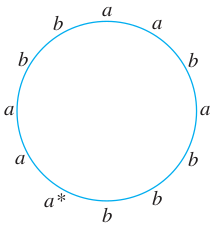
\includegraphics[scale=0.5]{../images/5.3.38.png}
\end{figure}

{\it Hint:} Given $k + 1$ $a$’s and $k + 1$ $b$’s arrayed around the outside of the circle, there has to be at least one location where an $a$ is followed by a $b$ as one travels in the clockwise direction. In the inductive step, temporarily remove such an $a$ and the $b$ that follows it, and apply the inductive hypothesis.

\begin{proof}
Let the property $P(n)$ be ``given $n$ $a$'s and $n$ $b$'s distributed around the outside of a circle, it is possible to find a starting point so that if you travel around the circle in a clockwise direction, the number of $a$'s you pass is never less than the number of $b$'s you have passed.''.

{\bf Show that $P(1)$ is true:} Given one $a$ and one $b$ we can start from the $a$ and go clockwise:

\begin{figure}[ht!]
\centering
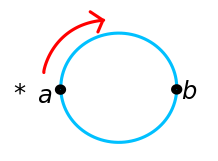
\includegraphics[scale=0.5]{../images/5.3.38.a.png}
\end{figure}

Then the number of $a$'s we pass will be 1 after we pass through the $a$, and the number of $b$'s we have passed at that point is 0, and 1 is not less than 0. So $P(1)$ is true.

{\bf Show that for every integer $k$ with $k \geq 1$, if $P(k)$ is true then $P(k+1)$ is true:} Assume $P(k)$ is true. Assume we are given $k+1$ $a$'s and $k+1$ $b$'s arranged around the outside of a circle.

On the circle, there must be at least one $a$ which is next to a $b$ when we are going clockwise. Removing that $a$ and $b$ leaves us with $k$ $a$'s and $k$ $b$'s. By the inductive hypothesis, it is possible to find a starting point so that if you travel around the circle in a clockwise direction, the number of $a$'s you pass is never less than the number of $b$'s you have passed. Mark this starting point with an asterisk *:

\begin{figure}[ht!]
\centering
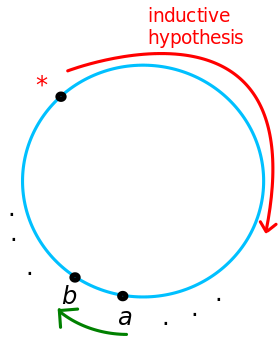
\includegraphics[scale=0.5]{../images/5.3.38.b.png}
\end{figure}

Now if we add back the $a$ and the $b$ that we removed, start from the same point at * and go clockwise, and go over the previously removed $a$ and $b$, it is still true that the number of $a$'s you pass is never less than the number of $b$'s you have passed (because we will pass over the $a$ first). This proves $P(k+1)$, {\it [as was to be shown.]}
\end{proof}

\subsection{Exercise 39}
For a polygon to be convex means that given any two points on or inside the polygon, the line joining the points lies entirely inside the polygon. Use mathematical induction to prove that for every integer $n \geq 3$, the angles of any $n$-sided convex polygon add up to $180(n - 2)$ degrees.

\begin{proof}
Let the property $P(n)$ be: ``the angles of any $n$-sided convex polygon add up to $180(n - 2)$ degrees.''

{\bf Show that $P(3)$ is true:} $P(3)$ says ``the angles of any triangle add up to $180(3 - 2) = 180$ degrees.'' This is true by our knowledge from high school geometry.

{\bf Show that for every integer $k \geq 3$, if $P(k)$ is true then $P(k+1)$ is true:} Suppose $k$ is an integer with $k \geq 3$ and suppose the angles of any $k$-sided convex polygon add up to $180(k - 2)$ degrees. {\it [We want to show that the angles of any $k+1$-sided convex polygon add up to $180(k+1 - 2)$ degrees.]}

Consider any $k+1$-sided convex polygon. Choose any two adjacent edges and connect them with a third edge (see below).

\begin{figure}[ht!]
\centering
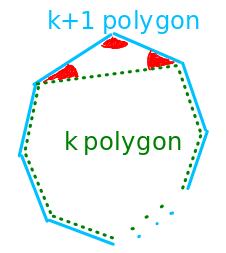
\includegraphics[scale=0.5]{../images/5.3.39.png}
\end{figure}

Since the polygon is convex, this splits the $k+1$-sided polygon (cyan) into two parts: a $k$-sided polygon (green), and a triangle (with red angles). By the inductive hypothesis, the angles of the $k$-sided (green) polygon add up to $180(k - 2)$ degrees. 

Now observe that the sum of the angles of the $k+1$-sided (cyan) polygon is equal to: 

the sum of the angles of the $k$-sided polygon (green) $ = 180(k-2)$

PLUS 

the sum of the angles of the triangle (red) $ = 180$

which equals $180(k-2) + 180 = 180(k+1-2)$ {\it [as was to be shown.]}
\end{proof}

\subsection{Exercise 40}
\subsubsection{(a)}
Prove that in an $8 \times 8$ checkerboard with alternating black and white squares, if the squares in the top right and bottom left corners are removed the remaining board cannot be covered with dominoes. ({\it Hint:} Mathematical induction is not needed for this proof.)

\begin{proof}
Let us consider an $8 \times 8$ checkerboard with alternating black and white squares. Thus, the checkerboard has total 64 squares, with 32 black and 32 white in color. Now, if the squares in the top right and bottom left corners are removed, both the removed ones are either black or white in color. Therefore, out of the remaining 62 squares, 30 squares are of one color and 32 are of other. Now a domino always covers one black and one white square. Thus, the board with 30 of one color and 32 of other cannot be covered with dominoes.
\end{proof}

\subsubsection{(b)}
Use mathematical induction to prove that for each positive integer $n$, if a $2n \times 2n$ checkerboard with alternating black and white squares has one white square and one black square removed anywhere on the board, the remaining squares can be covered with dominoes.

{\it Hint:} In the inductive step, imagine dividing a $2(k + 1) \times 2(k + 1)$ checkerboard into two sections: a center checkerboard of dimensions $2k \times 2k$ and an outer perimeter of single, adjacent squares. Then examine three cases: case 1 is where both removed squares are in the central $2k \times 2k$ checkerboard, case 2 is where one removed square is in the central $2k \times 2k$ checkerboard and the other is on the perimeter, and case 3 is where both removed squares are on the perimeter.

\begin{proof}
Let the property $P(n)$ be: ``if a $2n \times 2n$ checkerboard with alternating black and white squares has one white square and one black square removed anywhere on the board, the remaining squares can be covered with dominoes.''

{\bf Show that $P(1)$ is true:} $P(1)$ says ``if a $2 \times 2$ checkerboard with alternating black and white squares has one white square and one black square removed anywhere on the board, the remaining squares can be covered with dominoes.''

A $2 \times 2$ alternating B \& W board looks like this:
\begin{tabular}{|c|c|}
\hline
\colsq{black} & \colsq{lightgray} \\
\hline
\colsq{lightgray} & \colsq{black} \\
\hline
\end{tabular}
This means that, if one white square and one black square are removed, then either a row or a column is removed. So the remaining row or column can be covered with one domino. So $P(1)$ is true.

{\bf Show that for every integer $k \geq 1$, if $P(k)$ is true then $P(k+1)$ is true:} Assume $k \geq 1$ is an integer such that if a $2k \times 2k$ checkerboard with alternating black and white squares has one white square and one black square removed anywhere on the board, the remaining squares can be covered with dominoes.

{\it [We want to show that if a $2(k+1) \times 2(k+1)$ checkerboard with alternating black and white squares has one white square and one black square removed anywhere on the board, the remaining squares can be covered with dominoes.]}

(following the Hint) Split the $2(k+1) \times 2(k+1)$ board into two sections: a $2k \times 2k$ center, and the remaining perimeter surrounding it. For example, if $k = 3$ then it looks like this (for demonstration purposes, I colored the center yellow and the perimeter blue):

\begin{center}
\begin{tabular}{|c|c|c|c|c|c|c|c|}
\hline
\colsq{blue} & \colsq{blue} & \colsq{blue} & \colsq{blue} & \colsq{blue} & \colsq{blue} & \colsq{blue} & \colsq{blue}\\
\hline
\colsq{blue} & \colsq{yellow} & \colsq{yellow} & \colsq{yellow} & \colsq{yellow} & \colsq{yellow} & \colsq{yellow} & \colsq{blue}\\
\hline
\colsq{blue} & \colsq{yellow} & \colsq{yellow} & \colsq{yellow} & \colsq{yellow} & \colsq{yellow} & \colsq{yellow} & \colsq{blue}\\
\hline
\colsq{blue} & \colsq{yellow} & \colsq{yellow} & \colsq{yellow} & \colsq{yellow} & \colsq{yellow} & \colsq{yellow} & \colsq{blue}\\
\hline
\colsq{blue} & \colsq{yellow} & \colsq{yellow} & \colsq{yellow} & \colsq{yellow} & \colsq{yellow} & \colsq{yellow} & \colsq{blue}\\
\hline
\colsq{blue} & \colsq{yellow} & \colsq{yellow} & \colsq{yellow} & \colsq{yellow} & \colsq{yellow} & \colsq{yellow} & \colsq{blue}\\
\hline
\colsq{blue} & \colsq{yellow} & \colsq{yellow} & \colsq{yellow} & \colsq{yellow} & \colsq{yellow} & \colsq{yellow} & \colsq{blue}\\
\hline
\colsq{blue} & \colsq{blue} & \colsq{blue} & \colsq{blue} & \colsq{blue} & \colsq{blue} & \colsq{blue} & \colsq{blue}\\
\hline
\end{tabular}
\end{center}

Now consider the possibilities for the two removed squares.

{\bf Case 1: both removed squares are in the center.} Then by the inductive hypothesis, the $2k \times 2k$ center part with two squares removed (one white, one black) can be completely covered with dominoes. 

The perimeter can also be covered with dominoes: the top and bottom rows each have length $2(k+1)$ consisting of $k+1$ white squares and $k+1$ black squares, so they can be covered with $k+1$ dominoes each, and the remaining sides each have length $2k$ with $k$ white and $k$ black squares, which can be covered with $k$ dominoes each. 

Therefore the whole $2(k+1) \times 2(k+1)$ board (with one black, one white square removed) can be covered with dominoes, {\it [as was to be shown.]}

{\bf Case 2: both removed squares are on the perimeter.} The center $2k \times 2k$ part can be covered with dominoes since it has nothing removed. Now since one black and one white square are removed from the perimeter, the two ``paths'' along the perimeter between the two removed squares must each have even lengths, each containing equal numbers of white and black squares. 

For example, in the following picture the removed squares are shown as ``B'' and ``W'' and the others are shown in black and white, except the center which is not shown:

\begin{center}
\begin{tabular}{|c|c|c|c|c|c|c|c|}
\hline
\colsq{black} & \colsq{lightgray} & \colsq{black} & \colsq{lightgray} & \colsq{black} & \colsq{lightgray} & \colsq{black} & \colsq{lightgray} \\
\hline
\colsq{lightgray} &  &  &  &  &  &  & \colsq{black} \\
\hline
B &  &  &  &  &  &  & \colsq{lightgray} \\
\hline
\colsq{lightgray} &  &  &  &  &  &  & \colsq{black} \\
\hline
\colsq{black} &  &  &  &  &  &  & \colsq{lightgray} \\
\hline
\colsq{lightgray} &  &  &  &  &  &  & \colsq{black} \\
\hline
\colsq{black} &  &  &  &  &  &  & \colsq{lightgray} \\
\hline
\colsq{lightgray} & \colsq{black} & \colsq{lightgray} & \colsq{black} & \colsq{lightgray} & \colsq{black} & W & \colsq{black} \\
\hline
\end{tabular}
\end{center}

So both of those ``paths'' can be covered by dominoes, since they have even lengths, no gaps, and equal numbers of white and black squares. Hence the whole $2(k+1) \times 2(k+1)$ board can be covered, {\it [as was to be shown.]}

{\bf Case 3: one removed square is in the center, the other on the perimeter.} Consider the two squares removed, say P is removed from the perimeter, and C is removed from the center. 

If P and C are close enough to each other, so that they are both inside a $2k \times 2k$ square (not the center but some other $2k \times 2k$ square), then by the inductive hypothesis, that $2k \times 2k$ square can be covered with dominoes, and the remaining portion of the $2(k+1) \times 2(k+1)$ square can also be covered with dominoes since it has equal numbers of white and black squares, and no gaps. Here is an example with $k = 3$:

\begin{figure}[ht!]
\centering
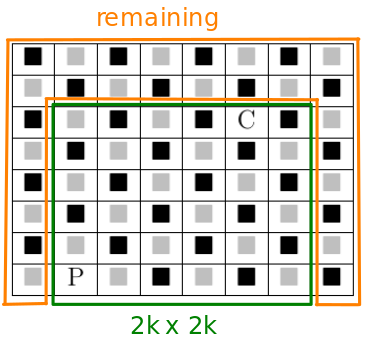
\includegraphics[scale=0.5]{../images/5.3.40.b.1.png}
\end{figure}

So we may assume that P and C do not fall into a $2k \times 2k$ square. In other words, we may assume that C is at the opposite end of the center from P, so that either horizontally or vertically, there are $2k-1$ squares between P and C. 

Since P and C have different colors, they cannot be on the same diagonal, so P and C always fit inside a $2k \times (2k+1)$ or a $(2k+1) \times 2k$ rectangle. Here are some examples for $k = 1$ to illustrate this. They always fit into either a $2 \times 3$ or a $3 \times 2$ rectangle:

\begin{figure}[ht!]
\centering
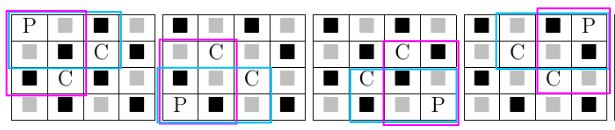
\includegraphics[scale=0.6]{../images/5.3.40.b.2.png}
\end{figure}

We cannot apply the inductive hypothesis to this $2k \times (2k+1)$ or $(2k+1) \times 2k$ rectangle. So we have to move C closer to P by one diagonal, so that the horizontal or vertical distance is $2k-2$ and hence they fall into a $2k \times 2k$ square. Here is an example for $k = 2$:

\begin{figure}[ht!]
\centering
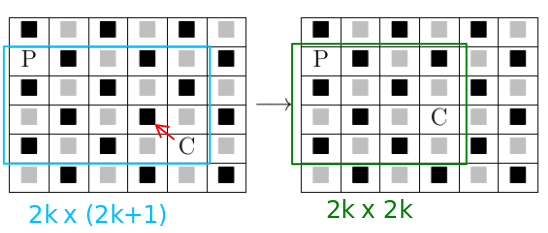
\includegraphics[scale=0.5]{../images/5.3.40.b.3.png}
\end{figure}

(Of course, depending on the position of P, we might have to move C in any one of the 4 diagonal directions. The picture above is only one example.)

Now we have to show that, this $2k \times (2k+1)$ or $(2k+1) \times 2k$ rectangle can be covered by dominoes, if and only if, the $2k \times 2k$ square obtained by moving C diagonally closer to P can be covered by dominoes. (This is possible but the proof is annoying and complicated, so I'll skip it here.)

By the inductive hypothesis, any $2k \times 2k$ board with one white and one black square removed can be covered with dominoes. Thus, by the above ``if and only if'' equivalence, the $2k \times (2k+1)$ or $(2k+1) \times 2k$ board can also be covered by dominoes. The remaining portion of the $2(k+1) \times 2(k+1)$ board can also be covered by dominoes, like before. So the whole $2(k+1) \times 2(k+1)$ board can be covered by dominoes, {\it [as was to be shown.]}
\end{proof}

\subsection{Exercise 41}
A group of people are positioned so that the distance between any two people is different from the distance between any other two people. Suppose that the group contains an odd number of people and each person sends a message to their nearest neighbor. Use mathematical induction to prove that at least one person does not receive a message from anyone. [This exercise is inspired by the article “Odd Pie Fights” by L. Carmony, The Mathematics Teacher, 72(1), 1979, 61–64.]

{\it Hint:} Let $P(n)$ be the sentence: If (1) $2n + 1$ people are all positioned so that the distance between any two people is different from the distance between any two other people, and if (2) each person sends a message to their nearest neighbor, then there is at least one person who does not receive a message from anyone. Use mathematical induction to prove that $P(n)$ is true for each integer $n \geq 1$.

\begin{proof}
(following the Hint) Let $P(n)$ be the sentence: ``If (1) $2n + 1$ people are all positioned so that the distance between any two people is different from the distance between any two other people, and if (2) each person sends a message to their nearest neighbor, then there is at least one person who does not receive a message from anyone.''

{\bf Show that $P(0)$ is true:} $P(0)$ says: ``If (1) $2 \cdot 0 + 1$ people are all positioned so that the distance between any two people is different from the distance between any two other people, and if (2) each person sends a message to their nearest neighbor, then there is at least one person who does not receive a message from anyone.'' 

Now the group has only $2 \cdot 0 + 1 = 1$ person and this person does not receive a message from anyone. So $P(0)$ is true.

{\bf Show that for every integer $k \geq 0$ if $P(k)$ is true then $P(k+1)$ is true:}

Suppose $k\geq 0$ is an integer such that $P(k)$ is true: if (1) $2k + 1$ people are all positioned so that the distance between any two people is different from the distance between any two other people, and if (2) each person sends a message to their nearest neighbor, then there is at least one person who does not receive a message from anyone. {\it [We want to show $P(k+1)$ is true.]}

To prove $P(k+1)$, suppose (1) $2(k+1) + 1$ people are all positioned so that the distance between any two people is different from the distance between any two other people, and (2) each person sends a message to their nearest neighbor.

{\it [Then we want to show there is at least one person who does not receive a message from anyone.]}

{\it [how to continue ??? Remove two people, use inductive hypothesis?]}
\end{proof}

\subsection{Exercise 42}
Show that for any (positive) even integer $n$, it is possible to find a group of $n$ people who are all positioned so that the distance between any two people is different from the distance between any other two people, so that each person sends a message to their nearest neighbor, and so that every person in the group receives a message from another person in the group.

\begin{proof}
{\it ???}
\end{proof}

\subsection{Exercise 43}
Define a game as follows: You begin with an urn that contains a mixture of white and black balls, and during the game you have access to as many additional white and black balls as you might need. In each move you remove two balls from the urn without looking at their colors. If the balls
are the same color, you put in one black ball. If the balls are different colors, you put the white ball back into the urn and keep the black ball out. Because each move reduces the number of balls in the urn by one, the game will end with a single ball in the urn. If you know how many white balls and how many black balls are initially in the urn, can you predict the color of the ball at the end of the game? [This exercise is based on one described in “Why correctness must be a mathematical concern” by E. W. Dijkstra, www.cs.utexas.edu/users /EWD/transcriptions/EWD07xx/EWD720.html.]

\subsubsection{(a)}
Map out all possibilities for playing the game starting with two balls in the urn, then three balls, and then four balls. For each case keep track of the number of white and black balls you start with and the color of the ball at the
end of the game.

{\it Hint:}
\arrayrulecolor{cyan}
\begin{tabular}{|ccc|}
\hline
\multicolumn{3}{|c|}{\cy Two Balls} \\
\hline
WW & $\to$ & B \\
\hline
WB & $\to$ & W \\
\hline
BB & $\to$ & B \\
\hline
\end{tabular}
\begin{tabular}{|cc|cc|}
\hline
\multicolumn{4}{|c|}{\cy Summary} \\
\hline
\multicolumn{2}{|c|}{Start} & \multicolumn{2}{c|}{End} \\
\hline
W & B & W & B \\
\hline
2 & 0 & 0 & 1 \\
\hline
1 & 1 & 1 & 0 \\
\hline
0 & 2 & 0 & 1 \\
\hline
\end{tabular}
\arrayrulecolor{black} % change it back!

\begin{proof}
{\it ???}
\end{proof}

\subsubsection{(b)}
Does the number of white balls seem to be predictive? Does the number of black balls seem to be predictive? Make a conjecture about the color of the ball at the end of the game given the numbers of white and black balls at the beginning.

{\it Hint:} In all three cases when the urn initially contains an odd number of white balls, there is one white ball in the urn at the end of the game, and when the urn initially contains an even number of white balls, there is one black ball (i.e., zero white balls) in the urn at the end of the game.

\begin{proof}
{\it ???}
\end{proof}

\subsubsection{(c)}
Use mathematical induction to prove the conjecture you made in part (b).

\begin{proof}
{\it ???}
\end{proof}

\subsection{Exercise 44}
Let $P(n)$ be the following sentence: Given any graph $G$ with $n$ vertices satisfying the condition that every vertex of $G$ has degree at most $M$, then the vertices of $G$ can be colored with at most $M + 1$ colors in such a way that no two adjacent vertices have the same color. Use mathematical induction to prove this statement is true for every integer $n \geq 1$.

{\it Hint:} Given a graph $G$ satisfying the given condition, form a new graph $G'$ by deleting one vertex $v$ of $G$ and all the edges that are incident on $v$. Then apply the inductive hypothesis to $G'$.

\begin{proof}
{\bf Show that $P(1)$ is true:} Given any graph $G$ with 1 vertex satisfying the given condition, we can color this vertex with only 1 color (which is $\leq M+1$) so that no two adjacent vertices have the same color (since there are no two adjacent vertices at all). So $P(1)$ is true.

{\bf Show that for any integer $k \geq 1$, if $P(k)$ is true then $P(k+1)$ is true:} Assume $P(k)$ is true, {\it [we want to prove $P(k+1)$ is true].} To prove $P(k+1)$ assume $G$ is any graph with $k+1$ vertices with degree at most $M$. {\it [We want to show that the vertices of $G$ can be colored with at most $M+1$ colors so that no two adjacent vertices have the same color.]}


Form a new graph $G'$ by deleting one vertex $v$ of $G$ and all the edges that are incident on $v$. Now $G'$ has $k$ vertices with degree at most $M$. By the inductive hypothesis we can color the vertices of $G'$ with at most $M+1$ colors so that no two adjacent vertices have the same color.

{\it ???}
\end{proof}

{\bf \cy In order for a proof by mathematical induction to be valid, the basis statement must be true for $n = a$ and the argument of the inductive step must be correct for every integer $k \geq a$. In 45 and 46 find the mistakes in the “proofs” by mathematical induction.}

\subsection{Exercise 45}
{\bf “Theorem:”} For any integer $n \geq 1$, all the numbers in a set of n numbers are equal to each other.

{\bf “Proof (by mathematical induction):} It is obviously true that all the numbers in a set consisting of just one number are equal to each other, so the basis step is true. For the inductive step, let $A = \{a_1, a_2, \ldots, a_k, a_{k+1}\}$ be any set of $k + 1$ numbers. Form two subsets each of size $k$:
\[
B = \{a_1, a_2, a_3, \ldots, a_k\} \text{ and } C = \{a_1, a_3, a_4, \ldots, a_{k+1}\}.
\]
($B$ consists of all the numbers in $A$ except $a_{k+1}$, and $C$ consists of all the numbers in $A$ except $a_2$.) By inductive hypothesis, all the numbers in $B$ equal $a_1$ and all the numbers in $C$ equal $a_1$ (since both sets have only $k$ numbers). But every number in $A$ is in $B$ or $C$, so all the numbers in $A$ equal $a_1$; hence all are equal to each other.”

\begin{proof}
The inductive step fails for going from $n = 1$ to $n = 2$,
because when $k = 1$,
\[
A = \{a_1, a_2\} \text{ and } B = \{a_1\}
\]
and no set $C$ can be defined to have the properties claimed for the $C$ in the proof. The reason is that $C = \{a_1\} = B$, and so an element of $A$, namely $a_2$, is
not in either $B$ or $C$.

Since the inductive step fails for going from $n = 1$ to $n = 2$, the truth of the following statement is never proved: “All the numbers in a set of two numbers are equal to each other.” This breaks the sequence of inductive steps, and so none of the statements for $n > 2$ is proved true either.

Here is an explanation for what happens in terms of the
domino analogy. The first domino is tipped backward (the basis step is proved). Also, if any domino from the second onward tips backward (the inductive step works or $n \geq 2$). In this case, however, when the first domino is tipped backward, it does not tip the second domino backward. So only the first domino falls down; the rest remain standing.
\end{proof}

\subsection{Exercise 46}
{\bf “Theorem:”} For every integer $n \geq 1$, $3^n - 2$ is even. 

{\bf “Proof (by mathematical induction):} Suppose the theorem is true for an integer $k$, where $k \geq 1$. That is, suppose that $3^k - 2$ is even. We must show that $3^{k+1} - 2$ is even. Observe that $3^{k+1} - 2 = 3^k \cdot 3 - 2 = 3^k(1 + 2) - 2 = (3^k - 2) + 3^k \cdot 2$. Now $3^k - 2$ is even by inductive hypothesis and $3^k \cdot 2$ is even by inspection. Hence the sum of the two quantities is even (by Theorem 4.1.1). It follows that $3^{k+1} - 2$ is even, which is what we needed to show.”

{\it Hint:} Is the basis step true?

\begin{proof}
This proof starts at the inductive step, assuming $P(k)$ and proving $P(k+1)$. However, it does not prove the basis step. In fact, the basis step is false: when $n = 1$, $3^n - 2 = 3^1 - 2 = 1$ is odd.

(Even if the basis step were true, the proof is still incomplete as it's missing the basis step.)
\end{proof}

\section{Exercise Set 5.4}

\subsection{Exercise 1}
Suppose that $a_1, a_2, a_3, \ldots$ is a sequence defined
as follows:
\[
a_1 = 1, a_2 = 3, a_k = a_{k-2} + 2a_{k-1} \text{ for every integer $k \geq 3$.}
\]
Prove that $a_n$ is odd for every integer $n \geq 1$.

\begin{proof}
Let the property $P(n)$ be the sentence “$a_n$ is odd.”

{\bf Show that $P(1)$ and $P(2)$ are true:}

Observe that $a_1 = 1$ and $a_2 = 3$ and both 1 and 3 are odd. Thus $P(1)$ and $P(2)$ are true.

{\bf Show that for every integer $k \geq 2$, if $P(i)$ is true for each integer $i$ with $1 \leq i \leq k$, then $P(k + 1)$ is true:}

Let $k$ be any integer with $k \geq 2$, and suppose $a_i$ is odd for each integer $i$ with $1 \leq i \leq k$. {\it [This is the inductive hypothesis.]} We must show that $a_{k+1}$ is odd. 

We know that $a_{k+1} = a_{k-1} + 2a_k$ by definition of $a_1, a_2, a_3, \ldots$. Moreover, $k - 1$ is less than $k + 1$ and is greater than or equal to 1 (because $k \geq 2$). Thus, by inductive hypothesis, $a_{k-1}$ is odd. 

Also, every term of the sequence is an integer (being a sum of products of integers), and so $2a_k$ is even by definition of even. 

It follows that $a_{k+1}$ is the sum of an odd integer and an even integer and hence is odd by Theorem 4.1.2 (Exercise 30, Section 4.1). {\it [This is what was to be shown.]}
\end{proof}

\subsection{Exercise 2}
Suppose that $b_1, b_2, b_3, \ldots$ is a sequence defined
as follows:
\[
b_1 = 4, b_2 = 12, b_k = b_{k-2} + b_{k-1} \text{ for every integer $k \geq 3$.}
\]
Prove that $b_n$ is divisible by 4 for every integer $n \geq 1$.

\begin{proof}
Let the property $P(n)$ be the sentence “$b_n$ is divisible by 4.”

{\bf Show that $P(1)$ and $P(2)$ are true:}

Observe that $b_1 = 4$ and $b_2 = 12$ and both 4 and 12 are divisible by 4. Thus $P(1)$ and $P(2)$ are true.

{\bf Show that for every integer $k \geq 2$, if $P(i)$ is true for each integer $i$ with $1 \leq i \leq k$, then $P(k + 1)$ is true:}

Let $k$ be any integer with $k \geq 2$, and suppose $b_i$ is divisible by 4 for each integer $i$ with $1 \leq i \leq k$. {\it [This is the inductive hypothesis.]} We must show that $b_{k+1}$ is divisible by 4. 

We know that $b_{k+1} = b_{k-1} + b_k$ by definition of $b_1, b_2, b_3, \ldots$. Moreover, $k - 1$ and $k$ are both less than or equal to $k$ and are greater than or equal to 1 (because $k \geq 2$). Thus, by inductive hypothesis, $b_{k-1}$ and $b_k$ are divisible by 4. So by definition of divisible, $b_{k-1} = 4m$ and $b_k = 4n$ for some integers $m,n$. 

It follows that $b_{k+1} = b_{k-1} + b_k = 4m + 4n = 4(m+n)$ is divisible by 4 because $m+n$ is an integer. {\it [This is what was to be shown.]}
\end{proof}

\subsection{Exercise 3}
Suppose that $c_0, c_1, c_2, \ldots$ is a sequence defined
as follows:
\[
c_0 = 2, c_1 = 2, c_2 = 6, c_k = 3c_{k-3} \text{ for every integer $k \geq 3$.}
\]
Prove that $c_n$ is even for every integer $n \geq 0$.

\begin{proof}
Let the property $P(n)$ be the sentence “$c_n$ is even.”

{\bf Show that $P(0), P(1)$ and $P(2)$ are true:}

Observe that $c_0 = 2, c_1 = 2$ and $c_2 = 6$ and both 2 and 6 are even. Thus $P(0), P(1)$ and $P(2)$ are true.

{\bf Show that for every integer $k \geq 2$, if $P(i)$ is true for each integer $i$ with $0 \leq i \leq k$, then $P(k + 1)$ is true:}

Let $k$ be any integer with $k \geq 2$, and suppose $c_i$ is even for each integer $i$ with $0 \leq i \leq k$. {\it [This is the inductive hypothesis.]} We must show that $c_{k+1}$ is even. 

We have $c_{k+1} = 3c_{k-2}$ and $0 \leq k-2 \leq k$, therefore $c_{k-2}$ is even by inductive hypothesis. So $c_{k-2} = 2m$ for some integer $m$. Then $c_{k+1} = 3c_{k-2} = 3(2m) = 2(3m)$ where $3m$ is an integer. Thus $c_{k+1}$ is even. {\it [This is what was to be shown.]}
\end{proof}

\subsection{Exercise 4}
Suppose that $d_1, d_2, d_3, \ldots$ is a sequence defined
as follows:
\[
d_1 = \frac{9}{10}, d_2 = \frac{10}{11}, d_k = d_{k-1} \cdot d_{k-2} \text{ for every integer $k \geq 3$.}
\]
Prove that $0 < d_n \leq 1$ for every integer $n \geq 1$.

\begin{proof}
Let the property $P(n)$ be the inequality $d_n \leq 1$.

{\bf Show that $P(1)$ and $P(2)$ are true:}

Observe that $d_1 = 9/10$ and $d_2 = 10/11$ and both $9/10 \leq 1$ and $10 / 11 \leq 1$. Thus $P(1)$ and $P(2)$ are true.

{\bf Show that for every integer $k \geq 2$, if $P(i)$ is true for each integer $i$ with $1 \leq i \leq k$, then $P(k + 1)$ is true:}

Let $k$ be any integer with $k \geq 2$, and suppose $d_i \leq 1$ for each integer $i$ with $1 \leq i \leq k$. {\it [This is the inductive hypothesis.]} We must show that $d_{k+1} \leq 1$. 

Now, by definition of $d_1, d_2, d_3, \ldots$, $d_{k+1} = d_k \cdot d_{k-1}$. Moreover $d_k \leq 1$ and $d_{k-1} \leq 1$ by inductive hypothesis because both $k - 1$ and $k$ are less than or equal to $k$. 

Consequently, $d_{k+1} = d_k \cdot d_{k-1} \leq 1$ because if two positive numbers are each less than or equal to 1, then their product is less than or equal to 1. 

{\it [To see why this is so, note that if $0 < a \leq 1$ and $0 < b \leq 1$, then multiplying $a \leq 1$ by $b$ gives $ab \leq b$, and since $b \leq 1$, then, by transitivity of order, $ab \leq 1$.]} Thus the inductive step has been proved. 

{\it [Since we have proved both the basis step and the inductive step, we conclude that $d_n \leq 1$ for every integer $n \geq 1$.]}
\end{proof}

\subsection{Exercise 5}
Suppose that $e_0, e_1, e_2, \ldots$ is a sequence defined
as follows:
\[
e_0 = 12, e_1 = 29, e_k = 5e_{k-1} - 6e_{k-2} \text{ for every integer $k \geq 2$.}
\]
Prove that $e_n = 5 \cdot 3^n + 7 \cdot 2^n$ for every integer $n \geq 0$.

\begin{proof}
Let the property $P(n)$ be the equation $e_n = 5 \cdot 3^n + 7 \cdot 2^n$.

{\bf Show that $P(0)$ and $P(1)$ are true:}

We must show that $e_0 = 5 \cdot 3^0 + 7 \cdot 2^0$ and $e_1 = 5 \cdot 3^1 + 7 \cdot 2^1$. 
The left-hand side of the first equation is 12 (by definition of $e_0, e_1, e_2, \ldots$), and its right-hand side is $5 \cdot 1 + 7 \cdot 1 = 12$ also. 
The left-hand side of the second equation is 29 (by definition of $e_0, e_1, e_2, \ldots$), and its right-hand side is $5 \cdot 3 + 7 \cdot 2 = 29$ also. 
Thus $P(0)$ and $P(1)$ are true.

{\bf Show that for every integer $k \geq 1$, if $P(i)$ is true for each integer $i$ with $0 \leq i \leq k$, then $P(k + 1)$ is also true:} 

Let $k$ be any integer with $k \geq 1$ and suppose that $e_i = 5 \cdot 3^i + 7 \cdot 2^i$ for each integer $i$ with $0 \leq i \leq k$. {\it [This is the inductive hypothesis.]}
We must show that $e_{k+1} = 5 \cdot 3^{k+1} + 7 \cdot 2^{k+1}$. Now

\begin{center}
\begin{tabular}{rcll}
$\dps e_{k+1}$ & = & $\dps 5e_{k} - 6e_{k-1}$ & {\cy by definition of $e_0, e_1, e_2, \ldots$} \\
$\dps $ & = & $\dps 5(5 \cdot 3^k + 7 \cdot 2^k) - 6(5 \cdot 3^{k-1} + 7 \cdot 2^{k-1})$ & {\cy by inductive hypothesis} \\
$\dps $ & = & $\dps 25 \cdot 3^k + 35 \cdot 2^k - 30 \cdot 3^{k-1} - 42 \cdot 2^{k-1}$ & {\cy by distributing} \\
$\dps $ & = & $\dps 25 \cdot 3^k + 35 \cdot 2^k - 10 \cdot 3 \cdot 3^{k-1} - 21 \cdot 2 \cdot 2^{k-1}$ & {\cy by algebra} \\
$\dps $ & = & $\dps 25 \cdot 3^k + 35 \cdot 2^k - 10 \cdot 3^{k} - 21 \cdot 2^{k}$ & {\cy by laws of exponents} \\
$\dps $ & = & $\dps 15 \cdot 3^k + 14 \cdot 2^k$ & {\cy by combining like terms} \\
$\dps $ & = & $\dps 5 \cdot 3 \cdot 3^k + 7 \cdot 2 \cdot 2^k$ & {\cy by algebra} \\
$\dps $ & = & $\dps 5 \cdot 3^{k+1} + 7 \cdot 2^{k+1}$ & {\cy by laws of exponents} \\
\end{tabular}
\end{center}

{\it [as was to be shown].}
\end{proof}

\subsection{Exercise 6}
Suppose that $f_0, f_1, f_2, \ldots$ is a sequence defined
as follows:
\[
f_0 = 5, f_1 = 16, f_k = 7f_{k-1} - 10f_{k-2} \text{ for every integer $k \geq 2$.}
\]
Prove that $f_n = 3 \cdot 2^n + 2 \cdot 5^n$ for every integer $n \geq 0$.

\begin{proof}
Let the property $P(n)$ be the equation $f_n = 3 \cdot 2^n + 2 \cdot 5^n$.

{\bf Show that $P(0)$ and $P(1)$ are true:}

We must show that $f_0 = 3 \cdot 2^0 + 2 \cdot 5^0$ and $f_1 = 3 \cdot 2^1 + 2 \cdot 5^1$. 
The left-hand side of the first equation is 5 (by definition of $f_0, f_1, f_2, \ldots$), and its right-hand side is $3 \cdot 2^0 + 2 \cdot 5^0 = 3 + 2 = 5$ also. 
The left-hand side of the second equation is 16 (by definition of $f_0, f_1, f_2, \ldots$), and its right-hand side is $3 \cdot 2^1 + 2 \cdot 5^1 = 6 + 10 = 16$ also. 
Thus $P(0)$ and $P(1)$ are true.

{\bf Show that for every integer $k \geq 1$, if $P(i)$ is true for each integer $i$ with $0 \leq i \leq k$, then $P(k + 1)$ is also true:} 

Let $k$ be any integer with $k \geq 1$ and suppose that $f_i = 3 \cdot 2^i + 2 \cdot 5^i$ for each integer $i$ with $0 \leq i \leq k$. {\it [This is the inductive hypothesis.]}
We must show that $f_{k+1} = 3 \cdot 2^{k+1} + 2 \cdot 5^{k+1}$. Now

\begin{center}
\begin{tabular}{rcll}
$\dps f_{k+1}$ & = & $\dps 7f_{k} - 10f_{k-1}$ & {\cy by definition of $f_0, f_1, f_2, \ldots$} \\
$\dps $ & = & $\dps 7(3 \cdot 2^k + 2 \cdot 5^k) - 10(3 \cdot 2^{k-1} + 2 \cdot 5^{k-1})$ & {\cy by inductive hypothesis} \\
$\dps $ & = & $\dps 21 \cdot 2^k + 14 \cdot 5^k - 30 \cdot 2^{k-1} - 20 \cdot 5^{k-1}$ & {\cy by distributing} \\
$\dps $ & = & $\dps 21 \cdot 2^k + 14 \cdot 5^k - 15 \cdot 2 \cdot 2^{k-1} - 4 \cdot 5 \cdot 5^{k-1}$ & {\cy by algebra} \\
$\dps $ & = & $\dps 21 \cdot 2^k + 14 \cdot 5^k - 15 \cdot  2^{k} - 4 \cdot 5^{k}$ & {\cy by laws of exponents} \\
$\dps $ & = & $\dps 6 \cdot 2^k + 10 \cdot 5^k$ & {\cy by combining like terms} \\
$\dps $ & = & $\dps 3 \cdot 2 \cdot 2^k + 2 \cdot 5 \cdot 5^k$ & {\cy by algebra} \\
$\dps $ & = & $\dps 3 \cdot 2^{k+1} + 2 \cdot 5^{k+1}$ & {\cy by laws of exponents} \\
\end{tabular}
\end{center}

{\it [as was to be shown].}
\end{proof}

\subsection{Exercise 7}
Suppose that $g_1, g_2, g_3, \ldots$ is a sequence defined
as follows:
\[
g_1 = 3, g_2 = 5, g_k = 3g_{k-1} - 2g_{k-2} \text{ for every integer $k \geq 3$.}
\]
Prove that $g_n = 2^n + 1$ for every integer $n \geq 1$.

\begin{proof}
Let the property $P(n)$ be the equation $g_n = 2^n + 1$.

{\bf Show that $P(1)$ and $P(2)$ are true:}

We must show that $g_1 = 2^1 + 1$ and $g_2 = 2^2 + 1$. 
The left-hand side of the first equation is 3 (by definition of $g_1, g_2, g_3, \ldots$), and its right-hand side is $2^1 + 1 = 2 + 1 = 3$ also. 
The left-hand side of the second equation is 5 (by definition of $g_1, g_2, g_3, \ldots$), and its right-hand side is $2^2 + 1 = 4 + 1 = 5$ also. 
Thus $P(1)$ and $P(2)$ are true.

{\bf Show that for every integer $k \geq 2$, if $P(i)$ is true for each integer $i$ with $1 \leq i \leq k$, then $P(k + 1)$ is also true:} 

Let $k$ be any integer with $k \geq 2$ and suppose that $g_i = 2^i + 1$ for each integer $i$ with $1 \leq i \leq k$. {\it [This is the inductive hypothesis.]}
We must show that $g_{k+1} = 2^{k+1} + 1$. Now

\begin{center}
\begin{tabular}{rcll}
$\dps g_{k+1}$ & = & $\dps 3g_{k} - 2g_{k-1}$ & {\cy by definition of $g_1, g_2, g_3, \ldots$} \\
$\dps $ & = & $\dps 3(2^{k} + 1) - 2(2^{k-1} + 1)$ & {\cy by inductive hypothesis} \\
$\dps $ & = & $\dps 3 \cdot 2^k + 3 - 2^k - 2$ & {\cy by distributing} \\
$\dps $ & = & $\dps 2 \cdot 2^k + 1$ & {\cy by combining like terms} \\
$\dps $ & = & $\dps 2^{k+1} + 1$ & {\cy by laws of exponents} \\
\end{tabular}
\end{center}

{\it [as was to be shown].}
\end{proof}

\subsection{Exercise 8}
Suppose that $h_0, h_1, h_2, \ldots$ is a sequence defined
as follows:
\[
h_0 = 1, h_1 = 1, h_2 = 2, h_k = h_{k-1} + h_{k-2} + h_{k-3} \text{ for every integer $k \geq 3$.}
\]
\subsubsection{(a)}
Prove that $h_n \leq 3^n$ for every integer $n \geq 0$.

\begin{proof}
Let the property $P(n)$ be the inequality $h_n \leq 3^n$.

{\bf Show that $P(0), P(1)$ and $P(2)$ are true:}

We must show that $h_0 \leq 3^0, h_1 \leq 3^1$ and $h_2 \leq 3^2$. 
The first inequality is $h_0 = 1 \leq 1 = 3^0$ which is true since $1 \leq 1$.
The second inequality is $h_1 = 1 \leq 3 = 3^1$ which is true since $1 \leq 3$.
The third inequality is $h_2 = 2 \leq 9 = 3^2$ which is true since $2 \leq 9$.
Thus $P(0), P(1)$ and $P(2)$ are true.

{\bf Show that for every integer $k \geq 2$, if $P(i)$ is true for each integer $i$ with $0 \leq i \leq k$, then $P(k + 1)$ is also true:} 

Let $k$ be any integer with $k \geq 2$ and suppose that $h_i \leq 3^i$ for each integer $i$ with $0 \leq i \leq k$. {\it [This is the inductive hypothesis.]}
We must show that $h_{k+1} \leq 3^{k+1}$. Now

\begin{center}
\begin{tabular}{rcll}
$\dps h_{k+1}$ & = & $\dps h_{k} + h_{k-1} + h_{k-2}$ & {\cy by definition of $h_0, h_1, h_2, \ldots$} \\
$\dps $ & $\leq$ & $\dps 3^{k} + 3^{k-1} + 3^{k-2}$ & {\cy by inductive hypothesis} \\
$\dps $ & $\leq$ & $\dps 3^{k} + 3^{k} + 3^{k}$ & {\cy because $3^{k-1} \leq 3^k$ and $3^{k-2} \leq 3^k$} \\
$\dps $ & = & $\dps 3 \cdot 3^{k}$ & {\cy by combining like terms} \\
$\dps $ & = & $\dps 3^{k+1}$ & {\cy by laws of exponents} \\
\end{tabular}
\end{center}

{\it [as was to be shown].}
\end{proof}

\subsubsection{(b)}
Suppose that $s$ is any real number such that $s^3 \geq s^2 + s + 1$. (This implies that $2 > s > 1.83$.) Prove that $h_n \leq s^n$ for every integer $n \geq 2$.

\begin{proof}
Let the property $P(n)$ be the inequality $h_n \leq s^n$.

{\bf Show that $P(0), P(1)$ and $P(2)$ are true:}

We must show that $h_0 \leq s^0, h_1 \leq s^1$ and $h_2 \leq s^2$. 
The first inequality is $h_0 = 1 \leq 1 = s^0$ which is true since $1 \leq 1$.
The second inequality is $h_1 = 1 \leq s^1$ which is true since $1 \leq 1.83 < s$.
The third inequality is $h_2 = 2 \leq s^2$ which is true since $2 \leq (1.83)^2 = 3.3489 < s^2$.
Thus $P(0), P(1)$ and $P(2)$ are true.

{\bf Show that for every integer $k \geq 2$, if $P(i)$ is true for each integer $i$ with $0 \leq i \leq k$, then $P(k + 1)$ is also true:} 

Let $k$ be any integer with $k \geq 2$ and suppose that $h_i \leq s^i$ for each integer $i$ with $0 \leq i \leq k$. {\it [This is the inductive hypothesis.]}
We must show that $h_{k+1} \leq s^{k+1}$. Now

\begin{center}
\begin{tabular}{rcll}
$\dps h_{k+1}$ & = & $\dps h_{k} + h_{k-1} + h_{k-2}$ & {\cy by definition of $h_0, h_1, h_2, \ldots$} \\
$\dps $ & $\leq$ & $\dps s^{k} + s^{k-1} + s^{k-2}$ & {\cy by inductive hypothesis} \\
$\dps $ & $=$ & $\dps s^{k-2}(s^2 + s + 1)$ & {\cy by factoring $s^{k-2}$} \\
$\dps $ & $\leq$ & $\dps s^{k-2}(s^3)$ & {\cy by the fact $s^3 \geq s^2 + s + 1$} \\
$\dps $ & $=$ & $\dps s^{k+1}$ & {\cy by laws of exponents}
\end{tabular}
\end{center}

{\it [as was to be shown].}
\end{proof}

\subsection{Exercise 9}
Define a sequence $a_1, a_2, a_3, \ldots$ as follows:
\[
a_1 = 1, a_2 = 3, a_k = a_{k-1} + a_{k-2} \text{ for every integer $k \geq 3$.}
\]
(This sequence is known as the Lucas sequence.) Use strong
mathematical induction to prove that $a_n \leq (7/4)^n$ for every integer $n \geq 1$.

\begin{proof}
Let the property $P(n)$ be the inequality $a_n \leq (7/4)^n$.

{\bf Show that $P(1)$ and $P(2)$ are true:}

We must show that $a_1 \leq (7/4)^1$ and $a_2 \leq (7/4)^2$. 
The first inequality is $a_1 = 1 \leq 7/4 = (7/4)^1$ which is true since $1 \leq 7/4$.
The second inequality is $a_2 = 3 \leq 3.0625 = 49 / 16 = (7/4)^2$ which is true since $3 \leq 3.0625$.
Thus $P(1)$ and $P(2)$ are true.

{\bf Show that for every integer $k \geq 2$, if $P(i)$ is true for each integer $i$ with $1 \leq i \leq k$, then $P(k + 1)$ is also true:} 

Let $k$ be any integer with $k \geq 2$ and suppose that $a_i \leq (7/4)^i$ for each integer $i$ with $1 \leq i \leq k$. {\it [This is the inductive hypothesis.]}
We must show that $a_{k+1} \leq (7/4)^{k+1}$. Now

\begin{center}
\begin{tabular}{rcll}
$\dps a_{k+1}$ & = & $\dps a_{k} + a_{k-1}$ & {\cy by definition of $a_1, a_2, a_3, \ldots$} \\
$\dps $ & $\leq$ & $\dps (7/4)^{k} + (7/4)^{k-1}$ & {\cy by inductive hypothesis} \\
$\dps $ & $=$ & $\dps (7/4)^{k-1}(7/4 + 1)$ & {\cy by factoring $(7/4)^{k-1}$} \\
$\dps $ & $=$ & $\dps (7/4)^{k-1}(11/4)$ & {\cy by algebra} \\
$\dps $ & $\leq$ & $\dps (7/4)^{k-1}(49/16)$ & {\cy because $11/4 \leq 49/16$} \\
$\dps $ & $=$ & $\dps (7/4)^{k-1}(7/4)^2$ & {\cy by rewriting} \\
$\dps $ & $=$ & $\dps (7/4)^{k+1}$ & {\cy by laws of exponents}
\end{tabular}
\end{center}

{\it [as was to be shown].}
\end{proof}

\subsection{Exercise 10}
The introductory example solved with ordinary
mathematical induction in Section 5.3 can also be
solved using strong mathematical induction. Let $P(n)$
be “any $n$¢ can be obtained using a combination of
3¢ and 5¢ coins.” Use strong mathematical induction
to prove that $P(n)$ is true for every integer $n \geq 8$.

{\it Hint:} In the basis step, show that $P(8), P(9)$,
and $P(10)$ are all true. For the inductive step, note
that $k + 1 = [(k + 1) - 3] + 3$, and if $k \geq 10$, then
$(k + 1) - 3 \geq 8$.

\begin{proof}
{\bf Show that $P(8), P(9)$ and $P(10)$ are true:}
8¢ = 3¢ + 5¢ so $P(8)$ is true. 
9¢ = 3¢ + 3¢ + 3¢ so $P(9)$ is true. 
10¢ = 5¢ + 5¢ so $P(10)$ is true.

{\bf Show that for every $k \geq 10$, if $P(i)$ is true for every $i$ with $8 \leq i \leq k$ then $P(k+1)$ is true:}

Notice that $k - 2 \geq 8$, so by the inductive hypothesis, $(k-2)$¢ can be obtained using a combination of 3¢ and 5¢ coins. 
Notice that $k + 1 = (k-2) + 3$. So $(k+1)$¢ can be obtained from $(k-2)$¢ by adding one more 3¢ coin.
Therefore $(k+1)$¢ can be obtained using a combination of 3¢ and 5¢ coins, {\it [as was to be shown.]}
\end{proof}

\subsection{Exercise 11}
You begin solving a jigsaw puzzle by finding two pieces that match and fitting them together. 
Every subsequent step of the solution consists of fitting together two blocks, each of which is made up of one or more pieces that have previously been assembled. 
Use strong mathematical induction to prove that for every integer $n \geq 1$, the number of steps required to put together all $n$ pieces of a jigsaw puzzle is $n - 1$.

\begin{proof}
Let the property $P(n)$ be the sentence ``A jigsaw puzzle consisting of $n$ pieces takes $n - 1$ steps to put together.''

{\bf Show that $P(1)$ is true:}
A jigsaw puzzle consisting of just one piece does not
take any steps to put together. Hence it is correct to say
that it takes zero steps to put together.

{\bf Show that for every integer $k \geq 1$, if $P(i)$ is true for each integer $i$ with $1 \leq i \leq k$, then $P(k + 1)$ is true:}

Let $k$ be any integer with $k \geq 1$ and suppose that for
each integer $i$ with $1 \leq i \leq k$, a jigsaw puzzle consisting of $i$ pieces takes $i - 1$ steps to put together. {\it [This is the inductive hypothesis.]} 
We must show that a jigsaw puzzle consisting of $k + 1$ pieces takes $k$ steps to put together. 

Consider assembling a jigsaw puzzle consisting of $k + 1$ pieces. 
The last step involves fitting together two blocks. Suppose one of the blocks consists of $r$ pieces and the other consists of $s$ pieces. Then $r + s = k + 1$, and $1 \leq r \leq k$ and $1 \leq s \leq k$. 
Thus, by the inductive hypothesis, the numbers of steps required to assemble the blocks are $r - 1$ and $s - 1$, respectively. 
Then the total number of steps required to assemble the puzzle is $(r - 1) + (s - 1) + 1 = (r + s) - 1 = (k + 1) - 1 = k$ {\it [as was to be shown]}.
\end{proof}

\subsection{Exercise 12}
The sides of a circular track contain a sequence of $n$ cans of gasoline. For each integer $n \geq 1$, the total amount in the cans is sufficient to enable a certain car to make one complete circuit of the track. 
In addition, all the gasoline could fit into the car’s gas tank at one time. 
Use mathematical induction to prove that it is possible to find an initial location for placing the car so that it will be able to traverse the entire track by using the various amounts of gasoline in the cans that it encounters along the way.

{\it Hint:} For any collection of cans, at least one must
contain enough gasoline to enable the car to get to the
next can. (Why?) 
Imagine taking all the gasoline from that can and pouring it into the can that immediately proceeds it in the direction of travel around the track. 
{\it (I think ``precedes'' here is a typo in the book, I think they meant ``proceeds'' so I changed it.)}

\begin{proof}
Let $P(n)$ be the statement: ``It is possible to find an initial location for placing the car so that it will be able to traverse the entire track by using the various amounts of gasoline in the $n$ cans that it encounters along the way.''

{\bf Show that $P(1)$ is true:} In this case there is only one gasoline can. Let the initial location for the car to be this can. By the given assumption in the problem statement, the total amount in this can is sufficient to enable the car to make one complete circuit of the track. Therefore $P(1)$ is true.

{\bf Show that for any integer $k \geq 1$, if $P(k)$ is true then $P(k+1)$ is true:}

Assume $k \geq 1$ is any integer and assume $P(k)$ is true. Assume we are considering a circuit with $k+1$ gasoline cans. For convenience, label them $c_1, c_2, \ldots, c_{k+1}$ in the direction of the car's movement, and label their gasoline amounts as $g_1, g_2, \ldots, g_{k+1}$ respectively.

So the problem tells us that $g_1 + g_2 + \ldots + g_{k+1}$ is enough to allow the car make one complete track around the circuit.

{\bf Claim:} For any collection of cans, at least one must
contain enough gasoline to enable the car to get to the
next can.

{\it Proof of Claim.} Argue by contradiction and assume that no can contains enough gasoline to enable the car to get to the next can. Then the total amount in the cans is insufficient to enable the car to make one complete circuit, which is a contradiction to the fact given in the problem.

By the Claim, there exists a can, let's say $c_1$, that contains enough gasoline $g_1$ to reach the next can $c_2$ in the direction of movement.

Consider the circuit with $k$ gasoline cans obtained from the current track by combining the gasoline in $c_1$ and $c_2$ into $c_1$. This is a circuit with $k$ gasoline cans: we got rid of $c_2$ and now $c_1$ contains gasoline in the amount of $g_1 + g_2$. So the cans and their gasoline amounts are: $c_1: g_1 + g_2, c_3: g_3, c_4: g_4, \ldots, c_{k+1}: g_{k+1}$.

By the inductive hypothesis, there is an initial location in this $k$ can circuit, say at can $c_i$, that allows the car to make one complete track around this circuit.

Now we want to show that the same starting point, $c_i$, also works for our $k+1$ can circuit.

Let the car start at $c_i$. Then the car is able to travel to $c_1$ because the cans from $c_i$ up to $c_1$ have enough gasoline to allow the car to reach $c_1$ (by the inductive hypothesis). Some of this gasoline might be left over. When the car reaches $c_1$, say the remaining gasoline in the tank is $g$.  From this point on, we will talk about the two different circuit runs in parallel.

In the $k$ can circuit, now the car fuels up at can $c_1$ and receives $g_1 + g_2$ amount of gasoline. So $g + (g_1 + g_2)$ is enough to reach from $c_1$ to the next can, which is $c_3$ (by the inductive hypothesis). 

To explain this a little bit better, say the exact amount of gasoline required to go from $c_1$ to $c_2$ is $G_1$, and the exact amount of gasoline required to go from $c_2$ to $c_3$ is $G_2$. So by the paragraph above, $g + g_1 + g_2 \geq G_1 + G_2$. And then the car reaches $c_3$ with $g + g_1 + g_2 - G_1 - G_2$ left in the tank, which is enough to complete the circuit back to $c_i$ (by the inductive hypothesis).

In the $k+1$ can circuit, now the car fuels up at can $c_1$ and receives $g_1$ amount of gasoline. Now there is $g + g_1$ in the tank. We know that $g_1$ is enough to go from $c_1$ to $c_2$ (by the property of $c_1$), so $g_1 \geq G_1$. Therefore the car reaches $c_2$ no problem, because $g + g_1 \geq G_1$. (Notice that if $g_1 \geq G_1$ weren't true, then the car would have to rely on the previous leftover $g$ to make up for the difference to reach $c_2$, which might not have been enough, since $g$ might be 0.)

Continuing on the $k+1$ circuit: when the car reaches $c_2$ there is $g + g_1 - G_1$ left in the tank. Now the car fuels up at $c_2$ and receives $g_2$ from $c_2$, so there is $g + g_1 - G_1 + g_2$ in the tank.

From the $k$ can circuit we know $g + g_1 + g_2 \geq G_1 + G_2$ which implies $g + g_1 + g_2 - G_1 \geq G_2$. The left hand side is the amount the tank has at $c_2$ in the $k+1$ can circuit. So this amount $g + g_1 + g_2 - G_1$ is enough from $c_2$ to reach $c_3$. 

When the car reaches $c_3$ in the $k+1$ can circuit, there is $g + g_1 + g_2 - G_1 - G_2$ left in the tank, which is exactly the same as the $k$ can circuit, so it's enough to complete the track back to $c_i$.

This proves $P(k+1)$, {\it [as was to be shown.]}
\end{proof}

\subsection{Exercise 13}
Use strong mathematical induction to prove the existence part of the unique factorization of integers theorem (Theorem 4.4.5). In other words, prove that every integer greater than 1 is either a prime number or a product of prime numbers.

\begin{proof}
{\it Sketch of proof:} Given any integer $k > 1$, either $k$ is prime or $k$ is a product of two smaller positive integers, each greater than 1. 
In the former case, the property is true. 
In the latter case, the inductive hypothesis ensures that both factors of $k$ are products of primes and hence that $k$ is also a product of primes.

Let the property $P(n)$ be: ``There exist a positive integer $k$, distinct prime numbers $p_1, p_2, \ldots, p_k$, and positive integers $e_1, e_2, \ldots, e_k$ such that $n = p_1^{e_1} p_2^{e_2} p_3^{e_3} \cdots p_k^{e_k}$.''

{\bf Show that $P(2)$ is true:} We have $2 = 2^{1}$ so we can choose $k = 1$, $p_1 = 2$ and $e_1 = 1$. So $P(2)$ is true.

{\bf Show that for any integer $n > 1$ if $P(i)$ is true for all integers $i$ with $1 < i \leq n$ then $P(n+1)$ is true:}

Assume $n > 1$ is any integer and assume that for every integer $i$ with $1 < i \leq n$ there exist a positive integer $k_i$, distinct prime numbers $p_{1_i}, p_{2_i}, \ldots, p_{k_i}$ and positive integers $e_{1_i}, e_{2_i}, \ldots, e_{k_i}$ such that $i = p_{1_i}^{e_{1_i}} p_{2_i}^{e_{2_i}} p_{3_i}^{e_{3_i}} \cdots p_{k_i}^{e_{k_i}}$.

{\it [We want to show that there exist a positive integer $k$, distinct prime numbers $p_1, \ldots, p_k$, and positive integers $e_1, e_2, \ldots, e_k$ such that $n+1 = p_1^{e_1} p_2^{e_2} p_3^{e_3} \cdots p_k^{e_k}$.]}

{\bf Case 1: $n+1$ is prime.} Then $n + 1 = (n+1)^1$ so we can take $k = 1, p_1 = n+1, e_1 = 1$ which proves $P(n+1)$ is true.

{\bf Case 2: $n+1$ is composite.} By definition of composite $n+1 = ab$ for integers $a,b$ with $1 < a < n+1$ and $1 < b < n+1$.

By the inductive hypothesis $a = q_1^{f_1} q_2^{f_2} \cdots q_x^{f_x}$ and $b = r_1^{g_1} r_2^{g_2} \cdots r_y^{g_y}$ for some positive integers $x, y, f_1, \ldots, f_x, g_1, \ldots, g_y$ and some primes $q_1, \ldots, q_x, r_1, \ldots, r_y$. The primes $q_1, \ldots, q_x$ are distinct among themselves, and the primes $r_1, \ldots, r_y$ are distinct among themselves.

Then $n+1 = ab = q_1^{f_1} q_2^{f_2} \cdots q_x^{f_x} \cdot r_1^{g_1} r_2^{g_2} \cdots r_y^{g_y}$. 

Now some of the primes $q_i$ might be among the primes $r_j$. If so, we can combine the powers in this product. For example if $q_i = r_j$ then we can let $s_i = q_i, h_i = f_i + g_j$ and combine the product $q_i^{f_i} \cdot r_j^{g_j} = s_i^{f_i + g_j} = s_i^{h_i}$. 

This way, we obtain distinct primes $s_1, \ldots, s_z$ for some positive integer $z$, and positive integers $h_1, \ldots, h_z$ such that
\[
n+1 = ab = s_1^{h_1} \cdots s_z^{h_z}
\]
which proves $P(n+1)$, {\it [as was to be shown.]}
\end{proof}

\subsection{Exercise 14}
Any product of two or more integers is a result of successive multiplications of two integers at a time. For instance, here are a few of the ways in which $a_1, a_2, a_3, a_4$ might be computed: $(a_1 a_2)(a_3 a_4)$ or $((a_1 a_2) a_3) a_4)$ or $a_1((a_2 a_3) a_4)$. Use strong mathematical induction to prove that any product of two or more odd integers is odd.

\begin{proof}
Let the property $P(n)$ be the sentence “Any product of $n$ odd integers is odd.”

{\bf Show that $P(1)$ and $P(2)$ are true:}
$P(1)$ is true because any product of one odd integer is odd. 
$P(2)$ is true because any product of two odd integers is odd (Exercise 20, Section 4.2).

{\bf Show that for every integer $k \geq 1$, if $P(i)$ is true for each integer $i$ with $1 \leq i \leq k$ then $P(k + 1)$ is true:}

Let $k$ be any integer with $k \geq 1$, and suppose that
for each integer $i$ with $1 \leq i \leq k$, any product 
of $i$ odd integers is odd. {\it [Inductive hypothesis]} 

Consider any product $M$ of $k + 1$ odd integers. 
Some multiplication is the final one that is used to obtain $M$. 
Thus, there are integers $A$ and $B$ such that $M = AB$, 
and each of $A$ and $B$ is a product of between 1 and $k$ 
odd integers. 
(For instance, if $M = ((a_1a_2)a_3)a_4$, then $A = (a_1a_2)a_3$ and $B = a_4$.) 
By inductive hypothesis, each of $A$ and $B$ is odd, and, 
as in the basis step, we know that any product of two odd
integers is odd. Hence $M = AB$ is odd.
\end{proof}

\subsection{Exercise 15}
Define the “sum” of one integer to be that integer, and use strong mathematical induction to prove that for every integer $n \geq 1$, any sum of $n$ even integers is even.

\begin{proof}
Let $P(n)$ be the statement ``any sum of $n$ even integers is even.''

{\bf Show that $P(1)$ is true:} The sum of one even integer is equal to itself, which is even. Thus $P(1)$ is true.

{\bf Show that for every integer $k \geq 1$ if $P(i)$ is true for all integers $i$ with $1 \leq i \leq k$ then $P(k+1)$ is true:}

Assume $k \geq 1$ is an integer such that any sum of $i$ even integers is even, for any integer $i$ with $1 \leq i \leq k$. {\it [We want to show that any sum of $k+1$ even integers is even.]}

Consider any sum $S$ of $k+1$ even integers. 
Some addition is the final one that is used to obtain $S$. 
Thus, there are integers $A$ and $B$ such that $S = A + B$,
and each of $A$ and $B$ is a sum of between 1 and $k$ 
even integers. 
(For instance, if $S = ((a_1 + a_2) + a_3) + a_4$, then $A = (a_1 + a_2) + a_3$ and $B = a_4$.) 
By inductive hypothesis, each of $A$ and $B$ is even, and, 
we know that any sum of two even integers is even. Hence $S = A + B$ is even, {\it [as was to be shown.]}
\end{proof}

\subsection{Exercise 16}
Use strong mathematical induction to prove that for every integer $n \geq 2$, if $n$ is even, then any sum of $n$ odd integers is even, and if $n$ is odd, then any sum of $n$ odd integers is odd.

{\it Hint:} Let the property $P(n)$ be the sentence “If 
$n$ is even, then any sum of $n$ odd integers is even,
and if $n$ is odd, then any sum of $n$ odd integers is odd.”
For the inductive step, consider any sum $S$ of $k + 1$ odd integers. 
Some addition is the final one that is used to obtain $S$.
Thus, there are integers $A$ and $B$ such that $S = A + B$,
and $A$ is a sum of $r$ odd integers 
and $B$ is a sum of $(k + 1) - r$ odd integers. 
Consider the two cases where $k + 1$ is even and $k + 1$ is
odd, and for each case consider the two subcases where $r$
is even and where $r$ is odd.

\begin{proof}
(following the Hint)

{\bf Show that $P(2)$ is true:} 2 is even, so we need to show that any sum of 2 odd integers is even. Assume $m, n$ are two odd integers. 
{\it [We want to show $m+n$ is even.]} 
By definition of odd $m = 2a+1$ and $n = 2b+1$ for some integers $a,b$. 
Then $m+n = 2a+1 + 2b + 1 = 2(a+b+1)$ where $a+b+1$ is an integer (because $a$ and $b$ are integers). 
So by definition of even, $m+n$ is even. This proves $P(2)$.

{\bf Show that for every integer $k \geq 2$, if $P(i)$ is true for all integers $i$ with $2 \leq i \leq k$ then $P(k+1)$ is true:}

Assume $k \geq 2$ is any integer such that for all $i$ with $2 \leq i \leq k$, if $i$ is even then any sum of $i$ odd integers is even, and if $i$ is odd then any sum of $i$ odd integers is odd.

{\it [We want to show that if $k+1$ is even, then any sum of $k+1$ odd integers is even, and if $k+1$ is odd, then any sum of $k+1$ odd integers is odd.]}

Consider any sum $S$ of $k+1$ odd integers.
Some addition is the final one that is used to obtain $S$.
Thus, there are integers $A$ and $B$ such that $S = A + B$,
$A$ is a sum of $r$ odd integers and $B$ is a sum of $(k + 1) - r$ odd integers.

{\bf Case 1: $k+1$ is even.} {\it [We want to show that $S$ is even.]} 

{\bf Subcase 1.1: $r$ is even.}
Then $(k+1) - r$ is even. So both $A$ and $B$ are sums of an even number of odd integers.
By inductive hypothesis $A$ and $B$ are both even.
Therefore $S = A + B$ is even (a sum of two even integers),
{\it [as was to be shown.]}

{\bf Subcase 1.2: $r$ is odd.}
Then $(k+1) - r$ is odd. So both $A$ and $B$ are sums of an odd number of odd integers.
By inductive hypothesis $A$ and $B$ are both odd.
Therefore $S = A + B$ is even (a sum of two odd integers),
{\it [as was to be shown.]}

{\bf Case 2: $k+1$ is odd.} {\it [We want to show that $S$ is odd.]} 

{\bf Subcase 2.1: $r$ is even.}
Then $(k+1) - r$ is odd. 
So $A$ is a sum of an even number of odd integers, and 
$B$ is a sum of an odd number of odd integers.
By inductive hypothesis $A$ is even and $B$ is odd.
Therefore $S = A + B$ is odd 
(a sum of one even and one odd integers),
{\it [as was to be shown.]}

{\bf Subcase 2.2: $r$ is odd.}
Then $(k+1) - r$ is even. 
So $A$ is a sum of an odd number of odd integers, and 
$B$ is a sum of an even number of odd integers.
By inductive hypothesis $A$ is odd and $B$ is even.
Therefore $S = A + B$ is odd 
(a sum of one odd and one even integers),
{\it [as was to be shown.]}
\end{proof}

\subsection{Exercise 17}
Compute $4^1, 4^2, 4^3, 4^4, 4^5, 4^6, 4^7$, and $4^8$. 
Make a conjecture about the units digit of $4^n$ where $n$ is a positive integer. 
Use strong mathematical induction to prove your conjecture.

\begin{proof}
$4^1 = 4, 4^2 = 16, 4^3 = 64, 4^4 = 256, 4^5 = 1024, 4^6 = 4096, 4^7 = 16384, 4^8 = 65536$.

{\it Conjecture:} 
The units digit of $4^n$ equals 4 if $n$ is odd and equals 6 if $n$ is even, 
for all $n \geq 1$.

\underline{Proof by strong mathematical induction:} 
Let $P(n)$ be the statement: 
``The units digit of $4^n$ is 4 if $n$ is odd, 6 if $n$ is even.''

{\bf Show that $P(1)$ and $P(2)$ are true:} 
When $n = 1$, $4^n = 4^1 = 4$, so the units digit is 4.
When $n = 2$, $4^n = 4^2 = 16$, so the units digit is 6.
Therefore $P(1)$ and $P(2)$ are true.

{\bf Show that for all integers $k \geq 2$, if $P(i)$ is true for all integers $i$ with $1 \leq i \leq k$ then $P(k+1)$ is true:}

Let $k$ by any integer with $k \geq 2$, and suppose that for each integer $i$ 
with $1 \leq i \leq k$, the units digit of $4^i$ equals 4 if $i$ is odd and 
equals 6 if $i$ is even. {\it [Inductive hypothesis]} 
We must show that the units digit of $4^{k+1}$ equals 4 
if $k + 1$ is odd and equals 6 if $k + 1$ is even.

{\bf Case 1 ($k + 1$ is odd):} In this case, $k$ is even,
and so, by inductive hypothesis, the units digits of $4^k$ is 6. 
Thus $4^k = 10q + 6$ for some nonnegative integer $q$. It follows that 
$4^{k+1} = 4^k \cdot 4 = (10q + 6) \cdot 4 = 40q + 24 = 10(4q + 2) + 4$. 
Thus, the units digit of $4^{k+1}$ is 4.

{\bf Case 2 ($k + 1$ is even):} In this case, $k$ is odd,
and so, by inductive hypothesis, the units digits of $4^k$ is 4. 
Thus $4^k = 10q + 4$ for some nonnegative integer $q$. It follows that 
$4^{k+1} = 4^k \cdot 4 = (10q + 4) \cdot 4 = 40q + 16 = 10(4q + 1) + 6$. 
Thus, the units digit of $4^{k+1}$ is 6.

{\bf\it Conclusion:} Because cases 1 and 2 are the only 
possibilities and $4^{k+1}$ has one of the required forms
in each case, we have shown that $P(k + 1)$ is true.
\end{proof}

\subsection{Exercise 18}
Compute $9^0, 9^1, 9^2, 9^3, 9^4$, and $9^5$. Make a conjecture about the units digit of $9^n$ where $n$ is a positive integer. Use strong mathematical induction to prove your conjecture.

\begin{proof}
$9^0 = 1, 9^1 = 9, 9^2 = 81, 9^3 = 729, 9^4 = 6561, 9^5 = 59049$.

{\it Conjecture:} 
The units digit of $9^n$ equals 9 if $n$ is odd and equals 1 if $n$ is even, for $n \geq 0$.

\underline{Proof by strong mathematical induction:} 
Let $P(n)$ be the statement: 
``The units digit of $9^n$ is 9 if $n$ is odd, 1 if $n$ is even.''

{\bf Show that $P(0)$ and $P(1)$ are true:} 
When $n = 0$, $9^n = 9^0 = 1$, so the units digit is 1.
When $n = 1$, $9^n = 9^1 = 9$, so the units digit is 9.
Therefore $P(0)$ and $P(1)$ are true.

{\bf Show that for all integers $k \geq 1$, if $P(i)$ is true for all integers $i$ with $0 \leq i \leq k$ then $P(k+1)$ is true:}

Let $k$ by any integer with $k \geq 1$, and suppose that for each integer $i$ 
with $0 \leq i \leq k$, the units digit of $9^i$ equals 9 if $i$ is odd and 
equals 1 if $i$ is even. {\it [Inductive hypothesis]}
We must show that the units digit of $9^{k+1}$ equals 9 
if $k + 1$ is odd and equals 1 if $k + 1$ is even.

{\bf Case 1 ($k + 1$ is odd):} In this case, $k$ is even, and so, by inductive 
hypothesis, the units digits of $9^k$ is 1.
Thus $9^k = 10q + 1$ for some nonnegative integer $q$. It follows that 
$9^{k+1} = 9^k \cdot 9 = (10q + 1) \cdot 9 = 90q + 9 = 10(9q) + 9$. 
Thus, the units digit of $9^{k+1}$ is 9.

{\bf Case 2 ($k + 1$ is even):} In this case, $k$ is odd, and so, by inductive 
hypothesis, the units digits of $9^k$ is 9. 
Thus $9^k = 10q + 9$ for some nonnegative integer $q$. It follows that 
$9^{k+1} = 9^k \cdot 9 = (10q + 9) \cdot 9 = 90q + 81 = 10(9q + 8) + 1$. 
Thus, the units digit of $9^{k+1}$ is 1.

{\bf\it Conclusion:} Because cases 1 and 2 are the only 
possibilities and $9^{k+1}$ has one of the required forms
in each case, we have shown that $P(k + 1)$ is true.
\end{proof}

\subsection{Exercise 19}
Suppose that $a_1, a_2, a_3, \ldots$ is a sequence defined as follows:
\[
a_1 = 1, a_k = 2 \cdot a_{\floor{k/2}} \text{ for every integer } k \geq 2.
\]
Prove that $a_n \leq n$ for each integer $n \geq 1$.

\begin{proof}
Let the property $P(n)$ be the inequality $a_n \leq n$. {\cy $\from P(n)$} 

We will show that $P(n)$ is true for each integer $n \geq 1$. 

{\bf Show that $P(1)$ is true:} $a_1 = 1$ and $1 \leq 1$. So $P(1)$ is true.

{\bf Show that for every integer $k \geq 1$, if $P(i)$ is true for each integer
$i$ from 1 through $k$, then $P(k + 1)$ is true:} Let $k$ be any integer with
$k \geq 1$, and suppose that $a_i \leq i$ for each integer $i$ with 
$1 \leq i \leq k$. {\cy $\from$ inductive hypothesis}

We must show that $a_{k+1} \leq k + 1$. Now

\begin{center}
\begin{tabular}{rcll}
$\dps a_{k+1}$ & = & $\dps 2 \cdot a_{\floor{(k+1)/2}}$ & {\cy by definition of $a_1, a_2, a_3, \ldots$} \\
$\dps $ & $\leq$ & $\dps 2 \cdot \floor{(k+1)/2}$ & {\cy by inductive hypothesis} \\
$\dps $ & $=$ & $\dps 
\left\{
\begin{array}{lr}
2((k+1)/2) & \text{if $k$ is odd} \\
2(k/2) & \text{if $k$ is even} \\
\end{array}
\right.$ & {\cy by definition of floor} \\
$\dps $ & $=$ & $\dps 
\left\{
\begin{array}{lr}
k+1 & \text{if $k$ is odd} \\
k & \text{if $k$ is even} \\
\end{array}
\right.$ & {\cy by algebra} \\
$\dps $ & $\leq$ & $\dps k+1$ & {\cy because $k \leq k+1$}
\end{tabular}
\end{center}

Thus $a_{k+1} \leq k + 1$ {\it [as was to be shown].}
\end{proof}

\subsection{Exercise 20}
Suppose that $b_1, b_2, b_3, \ldots$ is a sequence defined as follows:
\[
b_1 = 0, b_2 = 3, b_k = 5 \cdot b_{\floor{k/2}} + 6 \text{ for every integer } k \geq 3.
\]
Prove that $b_n$ is divisible by 3 for each integer $n \geq 1$.

\begin{proof}
Let the property $P(n)$ be the statement $3 \mid b_n$. {\cy $\from P(n)$} 

We will show that $P(n)$ is true for each integer $n \geq 1$. 

{\bf Show that $P(1)$ and $P(2)$ are true:} 
$b_1 = 0 = 3 \cdot 0$ and $b_2 = 3 = 3 \cdot 1$. 
So $3 \mid b_1$ and $3 \mid b_2$. 
So $P(1)$ and $P(2)$ are true.

{\bf Show that for every integer $k \geq 2$, if $P(i)$ is
true for each integer $i$ from 1 through $k$, then $P(k + 1)$ is true:}

Let $k$ be any integer with $k \geq 2$, and suppose that
$3 \mid b_i$ for each integer $i$ with $1 \leq i \leq k$.
{\cy $\from$ inductive hypothesis}

We must show that $3 \mid b_{k+1}$. 

{\bf Case 1: $k$ is even.} 
Then $k = 2i$ for some integer $i$ with $1 \leq i < k$, and
$\dps \floor{(k+1)/2} = \floor{(2i+1)/2} = \floor{i+1/2} = i$.
By the inductive hypothesis, $3 \mid b_i$. So $b_i = 3m$ for some integer $m$. Then
\[
b_{k+1} = 5 \cdot b_{\floor{(k + 1)/2}} + 6 = 5 \cdot b_i + 6 = 5 \cdot (3m) + 6 = 3(5m + 2)
\]
so by definition of divides, $3 \mid b_{k+1}$, {\it [as was to be shown.]}

{\bf Case 2: $k$ is odd.} 
Then $k = 2i + 1$ for some integer $i$ with $1 \leq i < k$,
and $\dps \floor{(k + 1)/2} = \floor{(2i + 1 + 1)/2} = \floor{(2i + 2)/2} = \floor{i+1}= i+1$. 
Note that $i + 1 \leq k$.
By the inductive hypothesis, $3 \mid b_{i + 1}$. So $b_{i + 1} = 3m$ for some integer $m$. Then
\[
b_{k+1} = 5 \cdot b_{\floor{(k + 1)/2}} + 6 = 5 \cdot b_{i + 1} + 6 = 5 \cdot (3m) + 6 = 3(5m + 2)
\]
so by definition of divides, $3 \mid b_{k+1}$, {\it [as was to be shown.]}
\end{proof}

\subsection{Exercise 21}
Suppose that $c_0, c_1, c_2, c_3, \ldots$ is a sequence defined as follows:
\[
c_0 = 1, c_1 = 1, c_k = c_{\floor{k/2}} + c_{\ceil{k/2}}  \text{ for every integer } k \geq 2.
\]
Prove that $c_n = n$ for each integer $n \geq 1$.

\begin{proof}
Let the property $P(n)$ be the equality $c_n = n$. {\cy $\from P(n)$} 

We will show that $P(n)$ is true for each integer $n \geq 1$. 

{\bf Show that $P(1)$ is true:} 
$c_1 = 1$ so $P(1)$ is true.

{\bf Show that for every integer $k \geq 1$, if $P(i)$ is
true for each integer $i$ from 1 through $k$, then $P(k + 1)$ is true:}

Let $k$ be any integer with $k \geq 1$, and suppose that
$c_i = i$ for each integer $i$ with $1 \leq i \leq k$.
{\cy $\from$ inductive hypothesis}

We must show that $c_{k+1} = k+1$. 

{\bf Case 1: $k$ is even.} 
Then $k = 2i$ for some integer $i$ with $1 \leq i < k$. So: 

$\dps \floor{(k+1)/2} = \floor{(2i+1)/2} = \floor{i+1/2} = i$, and

$\dps \ceil{(k+1)/2} = \ceil{(2i+1)/2} = \ceil{i+1/2} = i+1$.

Notice that $i + 1 \leq k$.

By the inductive hypothesis, $c_i = i$ and $c_{i+1} = i+1$. Then
\[
c_{k+1} = c_{\floor{(k+1)/2}} + c_{\ceil{(k+1)/2}} = c_i + c_{i+1} = i + (i+1) = 2i+1 = k+1,
\]
{\it [as was to be shown.]}

{\bf Case 2: $k$ is odd.} 
Then $k = 2i + 1$ for some integer $i$ with $1 \leq i < k$. So: 

$\dps \floor{(k + 1)/2} = \floor{(2i + 1 + 1)/2} = \floor{i + 1} = i + 1$, and

$\dps \ceil{(k + 1)/2} = \ceil{(2i + 1 + 1)/2} = \ceil{i + 1} = i+1$.

Notice that $i + 1 \leq k$.

By the inductive hypothesis $c_{i+1} = i+1$. Then
\[
c_{k + 1} = c_{\floor{(k+1)/2}} + c_{\ceil{(k+1)/2}} = c_{i + 1} + c_{i + 1} = (i+1) + (i+1) = 2i+2 = k+1,
\]
{\it [as was to be shown.]}
\end{proof}

\subsection{Exercise 22}
One version of the game NIM starts with two piles of
objects such as coins, stones, or matchsticks. In each turn
a player is required to remove from one to three objects
from one of the piles. The two players take turns doing
this until both piles are empty. The loser is the first
player who can’t make a move. Use strong mathematical
induction to show that if both piles contain the same
number of objects at the start of the game, the player who 
goes second can always win.

\begin{proof}
Let $P(n)$ be the sentence 
\begin{center}
In this version of NIM, if both piles initially contain $n$ objects, the player who goes second can always win. 
\end{center}

We will prove that $P(n)$ is true for every integer $n \geq 0$.

{\bf Show that $P(0)$ is true:}

If neither pile contains any objects, the player who goes first automatically loses because of not being able to make a move. So the second player wins the game by default. Thus $P(0)$ is true. 

{\bf Show that for every integer $k \geq 0$, if $P(i)$ is true for each integer $i$ from 1 through $k$, then $P(k + 1)$ is true:}

Let $k$ be any integer with $k \geq 0$, and suppose: 
\begin{center}
In this version of NIM, for every integer $i$ with $0 \leq i \leq k$, 
if both piles initially contain $i$ objects, the player who goes second can always win. 
\end{center}
We must show that In this version of NIM, if both piles initially contain $k + 1$ objects, the player who goes second can always win. {\cy $\from P(k + 1)$}

So suppose both piles contain $k + 1$ objects, where $0 \leq i \leq k$, and 
suppose the first player removes $r$ objects from pile \#1, where $1 \leq r \leq 3$. 
If the second player removes $r$ objects from pile \#2, then both piles will 
have the same number of objects, namely $(k + 1) - r$, and $(k + 1) - r \leq k$ 
because $r \geq 1$. Thus, by inductive hypothesis, the second player can win.
\end{proof}

\subsection{Exercise 23}
Define a game $G$ as follows: Begin with a pile of $n$ stones and 0 points. In the first move split the pile into
two possibly unequal sub-piles, multiply the number of stones in one sub-pile times the number of stones in the
other sub-pile, and add the product to your score. In the second move, split each of the newly created piles into a
pair of possibly unequal sub-piles, multiply the number of stones in each sub-pile times the number of stones in the 
paired sub-pile, and add the new products to your score. Continue by successively splitting each newly created pile 
of stones that has at least two stones into a pair of sub-piles, multiplying the number of stones in each sub-pile 
times the number of stones in the paired sub-pile, and adding the new products to your score. The game $G$ ends 
when no pile contains more than one stone.

\subsubsection{(a)}
Play $G$ starting with 10 stones and using the following initial moves. In move 1 split the pile of 10 stones into two sub-piles with 3 and 7 stones respectively, compute $3 \cdot 7 = 21$, and find that your score is 21. In move 2 split the pile of 3 stones into two sub-piles, with 1 and 2 stones respectively, and split the pile of 7 stones into two sub-piles, with 4 and 3 stones respectively, compute $1 \cdot 2 = 2$ and $4 \cdot 3 = 12$, and find that your score is $21 + 2 + 12 = 35$. In move 3 split the pile of 4 stones into two sub-piles, each with 2 stones, and split the pile of 3 stones into two sub-piles, with 1 and 2 stones respectively, and find your new score. Continue splitting piles and computing your score until no pile has more than one stone. Show your final score along with a record of the numbers of stones in the piles you created with your moves.

\begin{proof}
\begin{figure}[ht!]
\centering
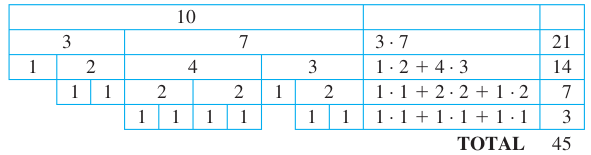
\includegraphics[scale=0.6]{../images/5.4.23.a.png}
\end{figure}
\end{proof}

\subsubsection{(b)}
Play $G$ again starting with 10 stones, but use a different initial move from the one in part (a). Show your final score along with a record of the numbers of stones in the piles you created with your moves.

\begin{proof}
\[
\arrayrulecolor{cyan}
\begin{array}{|c|c|c|c|c|c|c|c|c|c|c|c|}
\hline
\multicolumn{10}{|c|}{10} & & \\
\hline
\multicolumn{2}{|c}{2} & \multicolumn{8}{|c|}{8} & 2 \cdot 8 & 16 \\
\hline
1 & 1 & \multicolumn{4}{c|}{4} & \multicolumn{4}{c|}{4} & 1 \cdot 1 + 4 \cdot 4 & 17 \\
\hline
 &  & \multicolumn{2}{c|}{2} & \multicolumn{2}{c|}{2} & \multicolumn{2}{c|}{2} & \multicolumn{2}{c|}{2} & 2 \cdot 2 + 2 \cdot 2 & 8 \\
\hline
 &  & 1 & 1 & 1 & 1 & 1 & 1 & 1 & 1 & 1 \cdot 1 + 1 \cdot 1 + 1 \cdot 1 + 1 \cdot 1 & 4 \\
\hline
\end{array}
\arrayrulecolor{black}
\]
{\bf TOTAL} 45
\end{proof}

\subsubsection{(c)}
Show that you can use strong mathematical induction to prove that for every integer $n \geq 1$, given the set-up of game $G$, no matter how you split the piles in the various moves, your final score is $n(n - 1)/2$. The basis step may look a little strange because a pile consisting of one stone cannot be split into any sub-piles. Another way to say this is that it can only be split into zero piles, and that gives an answer that agrees with the general formula for the final score.

\begin{proof}
Let $P(n)$ be the statement: ``No matter how you split the piles in the various moves, your final score is $n(n-1)/2$.''

{\bf Show that $P(1)$ is true:} A pile of 1 stone cannot be split, therefore the score is 0, and $1(1-1)/2 = 0$ also. So $P(1)$ is true.

{\bf Show that for any integer $k \geq 1$ if $P(i)$ is true for all integers $i$ with $1 \leq i \leq k$ then $P(k+1)$ is true:}

Assume $k \geq 1$ is an integer and assume that for all integers $i$ with $1 \leq i \leq k$, a game played with 
starting $i$ stones, no matter how you split the piles in various moves, your final score is $i(i-1)/2$.

{\it [We want to show that in a game played with $k+1$ starting stones, no matter how you split the piles in
various moves, your final score is $(k+1)(k+2)/2$.]}

Starting with $k+1$ stones, there are $\dps \floor{\frac{k + 1}{2}}$ different ways to split the stones: 1 and $k$,
2 and $k-1$, 3 and $k-2, \ldots$, and $k/2$ and $k/2 + 1$ if $k+1$ is odd, $(k+1) / 2$ and $(k+1) / 2$ if $k+1$ is even.

In other words, the first move splits the stones into piles of $i$ and $(k+1) - i$ for some $1 \leq i \leq \floor{(k + 1) / 2}$. 
The score of this first move is $i(k+1-i) = ki + i - i^2$.

Then the rest of the game consists of two sub-games with starting piles of $i$ and $(k+1)-i$. By the inductive
hypothesis, no matter how you split the stones in these sub-games, the final scores are 
\[
\frac{i(i+1)}{2} = \frac{i^2 + i}{2}
\] 
and $\dps \frac{(k+1-i)(k+1-i+1)}{2}$
\[
= \frac{(k+1-i)(k+2-i)}{2} = \frac{k^2 + 2k - ik + k + 2 - i - ik - 2i + i^2}{2}
\] 
$\dps = \frac{k^2 + (3 - 2i)k + 2 - 3i + i^2}{2}$, respectively.

Then the total final score of the $k+1$ stone game is:
\[
ki + i - i^2 + \frac{i^2 + i}{2} + \frac{k^2 + (3 - 2i)k + 2 - 3i + i^2}{2} = \frac{k^2 + 3k + 2}{2}
\]
which is the same as the formula $(k+1)(k+2)/2$ that we claimed, {\it [as was to be shown.]}
\end{proof}

\subsection{Exercise 24}
Imagine a situation in which eight people, numbered consecutively $1-8$, are arranged in a circle. Starting from person \#1, every second person in the circle is eliminated. The elimination process continues until only one person remains. In the first round the people numbered 2, 4, 6, and 8 are eliminated, in the second round the people numbered 3 and 7 are eliminated, and in the third round person \#5 is eliminated, so after the third round only person \#1 remains, as shown below.

\begin{figure}[ht!]
\centering
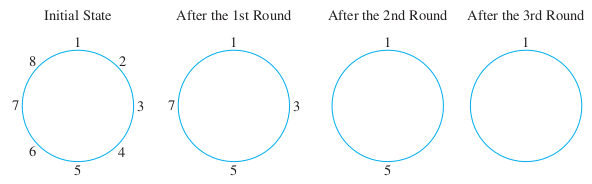
\includegraphics[scale=0.5]{../images/5.4.24.png}
\end{figure}

\subsubsection{(a)}
Given a set of sixteen people arranged in a circle and numbered, consecutively $1-16$, list the numbers of the people who are eliminated in each round if every second person is eliminated and the elimination process continues
until only one person remains. Assume that the starting point is person \#1.

\begin{proof}
The results are shown both diagrammatically and in a table (on the next page).

\begin{figure}[ht!]
\centering
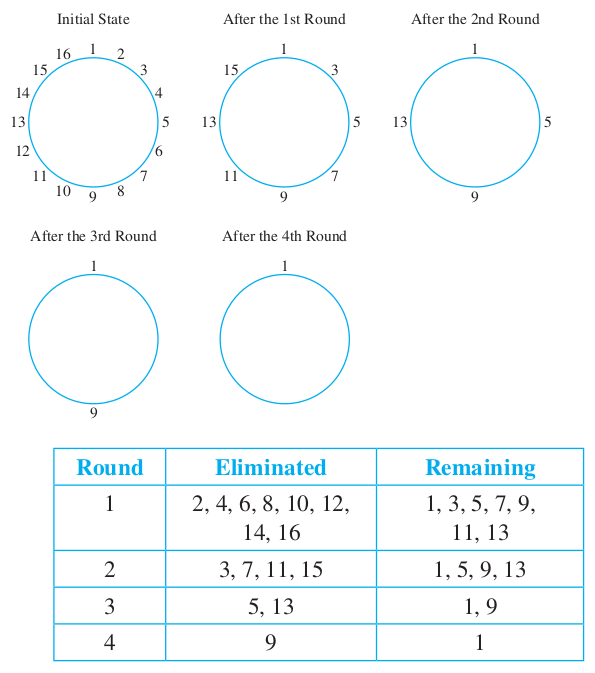
\includegraphics[scale=0.4]{../images/5.4.24.a.png}
\end{figure}
\end{proof}

\subsubsection{(b)}
Use ordinary mathematical induction to prove that for every integer $n \geq 1$, given any set of $2^n$ people arranged in a circle and numbered consecutively 1 through $2^n$, if one starts from person \#1 and goes repeatedly around the circle successively eliminating every second person, eventually only person \#1 will remain.

\begin{proof}
Let $P(n)$ be the statement ``given any set of $2^n$ people arranged in a circle and numbered consecutively 1 through
$2^n$, if one starts from person \#1 and goes repeatedly around the circle successively eliminating every second
person, eventually only person \#1 will remain.''

{\bf Show that $P(1)$ is true:} When $n = 1$ we have $2^n = 2^1 = 2$, so there are 2 people on the circle. 
Starting from person \#1, the second person is person \#2, who gets eliminated. So only person \#1 remains.
Thus $P(1)$ is true.

{\bf Show that for any integer $k \geq 1$, if $P(k)$ is true then $P(k+1)$ is true:}

Assume $k \geq 1$ is any integer and suppose that given any set of $2^k$ people arranged in a circle and numbered
consecutively 1 through $2^k$, if one starts from person \#1 and goes repeatedly around the circle successively 
eliminating every second person, eventually only person \#1 will remain.

Consider any set of $2^{k+1}$ people arranged in a circle and numbered consecutively 1 through $2^{k+1}$.
If we start from person \#1 and go repeatedly around the circle successively eliminating every second person,
then persons \#2, \#4, \#6, $\ldots$, \#$2^{k+1}$ will be eliminated.

This leaves us with a circle of the remaining $2^k$ people, numbered 1, 3, 5, 7, $\ldots$, $2^{k+1}-1$. 
By the inductive hypothesis, this game will result in only person \#1 remaining, {\it [as was to be shown.]}
\end{proof}

\subsubsection{(c)}
Use the result of part (b) to prove that for any nonnegative integers $n$ and $m$ with $2^n \leq 2^n + m < 2^{n+1}$, 
if $r = 2^n + m$, then given any set of $r$ people arranged in a circle and numbered consecutively 1 through $r$, 
if one starts from person \#1 and goes repeatedly around the circle successively eliminating every second person, eventually only person \#$(2m + 1)$ will remain.

\begin{proof}
{\it ???}
\end{proof}

\subsection{Exercise 25}
Find the mistake in the following “proof” that purports to show that every nonnegative integer power of every nonzero real number is 1.

{\bf “Proof:} Let $r$ be any nonzero real number and let the property $P(n)$ be the equation $r^n = 1$.

{\bf Show that $P(0)$ is true:} $P(0)$ is true because $r^0 = 1$ by definition of zeroth power.

{\bf Show that for every integer $k \geq 0$, if $P(i)$ is true for each integer $i$ from $0$ through $k$, then $P(k + 1)$ is also true:} Let $k$ be any integer with $k \geq 0$ and suppose that $r^i = 1$ for each integer $i$ from $0$ through $k$. This is the inductive hypothesis. We must show that $r^{k+1} = 1$. Now

\begin{center}
\begin{tabular}{rcll}
$\dps r^{k+1}$ & = & $\dps r^{k + k - (k - 1)}$ & {\cy because $k + k - (k - 1) = k+1$} \\
\vspace{0.3cm}
 & = & $\dps \frac{r^k \cdot r^k}{r^{k-1}}$ & {\cy by the laws of exponents} \\
 & = & $\dps \frac{1 \cdot 1}{1}$ & {\cy by inductive hypothesis} \\
 & = & $\dps 1.$ & {\cy by algebra} 
\end{tabular}
\end{center}

Thus $r^{k+1} = 1$ {\it [as was to be shown].}

{\it [Since we have proved the basis step and the inductive
step of the strong mathematical induction, we conclude that the given statement is true.]”}

\begin{proof}
The mistake is with the term $r^{k-1}$ being replaced by 1. Because, the assumption is that $k \geq 0$ and $P(i)$ is true for all $i$ with $0 \leq i \leq k$. So here the mistake is using $i = k-1$. When $k = 0$ we get $i = k - 1 = -1$ which does not satisfy $0 \leq i$. So we cannot apply the inductive hypothesis to $i = k-1$.
\end{proof}

\subsection{Exercise 26}
Use the well-ordering principle for the integers to prove Theorem 4.4.4: Every integer greater than 1 is divisible by a prime number.

\begin{proof}
Let $n$ be any integer greater than 1. Consider the set $S$ of all positive integers other than 1 that divide $n$. 
Since $n \mid n$ and $n > 1$, there is at least one element in $S$. Hence, by the well-ordering principle for the 
integers, $S$ has a smallest element; call it $p$. We claim that $p$ is prime. 

For suppose $p$ is not prime. Then there are integers $a$ and $b$ with $1 < a < p$, $1 < b < p$, and $p = ab$. By 
definition of divides, $a \mid p$. Also $p \mid n$ because $p$ is in $S$ and every element in $S$ divides $n$. 
Therefore, $a \mid p$ and $p \mid n$, and so, by transitivity of divisibility, $a \mid n$. Consequently, $a 
\in S$. But this contradicts the fact that $a < p$, and $p$ is the smallest element of $S$. 

{\it [This contradiction  shows that the supposition that $p$ is not prime is false.]} Hence $p$ is prime, and we 
have shown the existence of a prime number that divides $n$. 
\end{proof}

\subsection{Exercise 27}
Use the well-ordering principle for the integers to prove the existence part of the unique factorization of integers theorem. In other words, prove that every integer greater than 1 is either prime or a product of prime numbers.

\begin{proof}
Consider the set $S$ of integers that are greater than 1, not a prime, and not a product of prime numbers.

We claim that $S$ is empty. Argue by contradiction and assume $S$ is nonempty.

By the Well-Ordering Principle, $S$ has a smallest element, call it $a$. 
So $a > 1$ and $a$ is not prime and $a$ is not a product of primes.

Since $a$ is not prime, $a$ is composite. 
By definition of composite $a = bc$ for some integers $1 < b < a$ and $1 < c < a$.

By the minimality of $a$, it follows that $b$ and $c$ are either primes or products of primes. Then $a = bc$ is also
a product of primes, which is a contradiction.

{\it [Thus our initial supposition was false and $S$ is empty.]} So it follows that every integer greater than 1 is 
either prime or a product of primes, {\it [as was to be shown.]}
\end{proof}

\subsection{Exercise 28}

\subsubsection{(a)}
The Archimedean property for the rational numbers states that for every rational number $r$, there is an integer $n$ such that $n > r$. Prove this property.

\begin{proof}
Suppose $r$ is any rational number. {\it [We need to show that there is an integer $n$ such that $r < n$.]}

{\bf Case 1 ($r \leq 0$):} In this case, take $n = 1$. Then
$r < n$. 

{\bf Case 2 ($r > 0$):} In this case, $r = a/b$ for some positive integers $a$ and $b$ (by definition of rational
and because $r$ is positive). Note that $r = a/b < n$ if, and only if, $a < nb$. Let $n = 2a$. Multiply both sides of 
the inequality $1 < 2$ by $a$ to obtain $a < 2a$, and multiply both sides of the inequality $1 < b$ by $2a$ to 
obtain $2a < 2ab = nb$. Thus $a < 2a < nb$, and so, by transitivity of order, $a < nb$. Dividing both sides $a$ by 
$b$ gives that $a/b < n$, or, equivalently, that $r < n$. 

Hence, in both cases, $r < n$ {\it [as was to be shown].}
\end{proof}

\subsubsection{(b)}
Prove that given any rational number $r$, the number $-r$ is also rational.

\begin{proof}
Assume $r$ is any rational number.
By definition of rational $r = a/b$ for some integers $a,b$ with $b \neq 0$.
Then $-r = (-a)/b$ where $-a$ and $b$ are integers with $b \neq 0$.
So by definition of rational, $-r$ is rational.
\end{proof}

\subsubsection{(c)}
Use the results of parts (a) and (b) to prove that given any rational number $r$, there is an integer $m$ such that $m < r$.

\begin{proof}
Assume $r$ is any rational number.
By part (b), $-r$ is a rational number.
By part (a) applied to $-r$, there exists an integer $n$ such that $n > -r$. Let $m = -n$. 
Then multiply the inequality $n > -r$ by $-1$ to get $-n < r$, or equivalently, $m < r$, {\it [as was to be shown].}
\end{proof}

\subsection{Exercise 29}
Use the results of exercise 28 and the well-ordering principle for the integers to show that given any rational number $r$, there is an integer $m$ such that $m \leq r < m + 1$.

{\it Hint:} If $r$ is any rational number, let $S$ be the set of all integers $n$ such that $r < n$. 
Use the results of exercises 28(a), 28(c), and the well-ordering principle for the integers to show that $S$ has a
least element, say $v$, and then show that $v - 1 \leq r < v$.

\begin{proof}
(following the Hint)

Assume $r$ is any rational number. 
By Exercise 28 (c) there is an integer $n$ such that $n < r$.
Let $S$ be the set of integers that are greater than $n$ and greater than $r$. By Exercise 28 (a) $S$ is nonempty.
Since every integer in $S$ is greater than the fixed integer $n$, by the well-ordering principle, 
$S$ has a least element, call it $v$.
Then $r < v$ and by the minimality of $v$, $v-1 \leq r$.
Let $m = v-1$. Then $m$ is an integer, and $m \leq r < m+1$ {\it [as was to be shown].}

\end{proof}

\subsection{Exercise 30}
Use the well-ordering principle to prove that given any integer $n \geq 1$, there exists an odd integer $m$ and a nonnegative integer $k$ such that $n = 2^k \cdot m$.

\begin{proof}
Let $S$ be the set of all integers $r$ such that $n = 2^i \cdot r$ for some integer $i$. 
Then $n \in S$ because $n = 2^0 \cdot n$, and so $S \neq \emptyset$. 
Also, since $n \geq 1$, each $r$ in $S$ is positive, and so, by the well-ordering principle, $S$ has a least element 
$m$. 

This means that $n = 2^k \cdot m$ (*) for some nonnegative integer $k$, and $m \leq r$ for every $r$ in $S$. 

We claim that $m$ is odd. The reason is that if $m$ is even, then $m = 2p$ for some integer $p$. 
Substituting into equation (*) gives 
\[
n = 2^k \cdot m = 2^k \cdot 2p = (2^k \cdot 2)p = 2^{k+1} \cdot p.
\]
It follows that $p \in S$ and $p < m$, which contradicts the fact that $m$ is the least element of $S$. 
Hence $m$ is odd, and so $n = m \cdot 2^k$ for some odd integer $m$ and nonnegative integer $k$.
\end{proof}

\subsection{Exercise 31}
Give examples to illustrate the proof of Theorem 5.4.1.

\begin{proof}
Let $k = 25$ so $k+1 = 26$ is even. By the inductive hypothesis $(k+1)/2 = 13$ has a binary representation:
\[
13 = 8 + 4 + 1 = 1 \cdot 2^3 + 1 \cdot 2^2 + 0 \cdot 2^1 + 1 \cdot 2^0 = 1101_\base{2}.
\]
Multiply everything by 2 and add missing powers of 2:
\[
26 = 13 \cdot 2 = 16 + 8 + 2 = 1 \cdot 2^4 + 1 \cdot 2^3 + 0 \cdot 2^2 + 1 \cdot 2^1 + 0 \cdot 2^0 = 11010_\base{2}.
\]
Let $k = 14$ so $k+1 = 15$ is even. By the inductive hypothesis $k/2 = 7$ has a binary representation:
\[
7 = 4 + 2 + 1 = 1 \cdot 2^2 + 1 \cdot 2^1 + 1 \cdot 2^0 = 111_\base{2}.
\]
Multiply everything by 2 and add missing powers of 2:
\[
14 = 7 \cdot 2 = 8 + 4 + 2 = 1 \cdot 2^3 + 1 \cdot 2^2 + 1 \cdot 2^1 + 0 \cdot 2^0 = 1110_\base{2}.
\]
To get the binary representation of $k+1$, just add 1:
\[
15 = 14 + 1 = 1 \cdot 2^3 + 1 \cdot 2^2 + 1 \cdot 2^1 + 1 \cdot 2^0 = 1111_\base{2}.
\]
\end{proof}

\subsection{Exercise 32}
Suppose $P(n)$ is a property such that

1. $P(0), P(1), P(2)$ are all true,

2. for each integer $k \geq 0$, if $P(k)$ is true, then
$P(3k)$ is true. 

Must it follow that $P(n)$ is true for every integer $n \geq 0$? If yes, explain why; if no, give a counterexample.

\begin{proof}
No. Let $P(n)$ be the statement: ``either $n = 1$ or $n = 2$ or $3 \mid n$.''

Then $P(0), P(1)$ and $P(2)$ are all true, because $3 \mid 0$, and $1 = 1$ and $2 = 2$.

Assume $k \geq 0$ is an integer and $P(k)$ is true. {\it [We want to show $P(3k)$ is true.]}
$P(3k)$ is true because $3 \mid 3k$.

However it is not the case that $P(n)$ is true for every integer $n \geq 0$: for example $P(4)$ is false because $4 \neq 1$ and $4 \neq 2$ and $3 \nmid 4$.
\end{proof}

\subsection{Exercise 33}
Prove that if a statement can be proved by strong mathematical induction, then it can be proved by ordinary mathematical induction. To do this, let $P(n)$ be a property that is defined for each integer $n$, and suppose the following two statements are true:

1. $P(a), P(a + 1), P(a + 2), \ldots, P(b)$.

2. For any integer $k \geq b$, if $P(i)$ is true for each
integer $i$ from $a$ through $k$, then $P(k + 1)$ is true.

The principle of strong mathematical induction would allow us to conclude immediately that $P(n)$ is true for every integer $n \geq a$. Can we reach the same conclusion using the principle of ordinary mathematical induction? Yes! To see this, let $Q(n)$ be the property $P(j)$ is true for each integer $j$ with $a \leq j \leq n$. Then use ordinary mathematical induction to show that $Q(n)$ is true for every integer $n \geq b$. That is, prove:

1. $Q(b)$ is true.

2. For each integer $k \geq b$, if $Q(k)$ is true then $Q(k + 1)$ is true.

\begin{proof}
{\bf Show that $Q(b)$ is true:} $Q(b)$ is the statement ``$P(j)$ is true for each integer $j$ with $a \leq j \leq b$.'' 
This is true because we are assuming that $P(a), P(a + 1), P(a + 2), \ldots, P(b)$ are all true (1. given above).
Therefore $Q(b)$ is true.

{\bf Show that for each integer $k \geq b$, if $Q(k)$ is true then $Q(k+1)$ is true:}

Assume $k$ is an integer with $k \geq b$ and assume $Q(k)$ is true. By definition of $Q$, this means that $P(j)$ is
true for all integers $j$ with $a \leq j \leq k$.
So by 2. given in the exercise, $P(k+1)$ is true.
So $P(j)$ is true for all integers $j$ with $a \leq j \leq k+1$. Thus $Q(k+1)$ is true, {\it [as was to be shown].}
\end{proof}

\subsection{Exercise 34}
It is a fact that every integer $n \geq 1$ can be written
in the form
\[
c_r \cdot 3^r + c_{r-1} \cdot 3^{r-1} + \cdots + c_2 \cdot 3^2 + c_1 \cdot 3 + c_0,
\]
where $c_r = 1$ or $2$ and $c_i = 0, 1$, or $2$ for each
integer $i = 0, 1, 2, \ldots, r - 1$. Sketch a proof of this fact.

{\it Hint:} In the inductive step, divide into cases depending on whether $k+1$ can be written as $k+1 = 3x$ or 
$k+1 = 3x + 1$ or $k+1 = 3x + 2$ for some integer $x$.

\begin{proof}
Here is a sketch using strong induction. Let $P(n)$ be the statement ``$n$ can be written in the form given above.''

For the base cases, we need to prove $P(0), P(1)$ and $P(2)$. This is easily verified manually.

For the inductive step, assume $P(i)$ is true for all $i$ from 0 through $k$. To show $P(k+1)$ consider 3 cases:

$k + 1 = 3x$: Say we have, by inductive hypothesis applied to $(k+1)/3$,
\[
(k + 1) / 3 = c_r \cdot 3^r + c_{r-1} \cdot 3^{r-1} + \cdots + c_2 \cdot 3^2 + c_1 \cdot 3 + c_0.
\]
Then multiplying by 3 we get
\[
k + 1 = c_r \cdot 3^{r+1} + c_{r-1} \cdot 3^{r} + \cdots + c_2 \cdot 3^3 + c_1 \cdot 3^2 + c_0 \cdot 3^1 + 0.
\]
Thus we get the representation for $k+1$.

$k + 1 = 3x+1$: Similar, but start by using inductive hypothesis applied to $k/3$ instead, then add 1.

$k + 1 = 3x+2$: Similar, but start by using inductive hypothesis applied to $(k-1)/3$ instead, then add 2.
\end{proof}

\subsection{Exercise 35}
Use mathematical induction to prove the existence part of the quotient-remainder theorem. In other words, use mathematical induction to prove that given any integer $n$ and any positive integer $d$, there exist integers $q$ and $r$ such that $n = dq + r$ and $0 \leq r < d$.

{\it Hint:} In the inductive step, let an integer $k \geq 0$ be given and suppose that there exist integers $q'$ and
$r'$ such that $k = dq' + r'$ and $0 \leq r' < d'.$ You must show that there exist integers $q$ and $r$ such that
\[
k + 1 = dq + r \text{ and } 0 \leq r < d.
\]
To do this, consider the two cases $r' < d - 1$ and $r' = d - 1$.

\begin{proof}
We will prove this for nonnegative integers $n$ first. Then we'll use that to prove it in general.

Let $P(n)$ be the statement: ``for any positive integer $d$, there exist integers $q$ and $r$ such that $n = dq + r$ and $0 \leq r < d$.''

{\bf Show that $P(0)$ is true:} Let $q = r = 0$. Then $dq + r = d \cdot 0 + 0 = 0 = n$ so $P(0)$ is true.

{\bf Show that for any integer $k \geq 0$ if $P(k)$ is true then $P(k+1)$ is true:} (following the Hint)

Let an integer $k \geq 0$ be given and suppose that there exist integers $q'$ and $r'$ such that $k = dq' + r'$ and 
$0 \leq r' < d'.$ {\it [We must show that there exist integers $q$ and $r$ such that]}
\[
k + 1 = dq + r \text{ and } 0 \leq r < d.
\]
{\bf Case 1: $r' < d - 1$.} Then let $q = q'$ and $r = r'+1$. So we have
\[
k+1 = (dq' + r') + 1 = dq' + (r' + 1) = dq + r
\]
and since $r' < d-1$ we have $r = r'+1 < d$, so this proves $P(k+1)$.

{\bf Case 2: $r' = d - 1$.} Notice that $r' + 1 = d$. Let $q = q'+1$ and $r = 0$.  Then
\[
k+1 = (dq'+r') + 1 = dq' + (r'+1) = dq'+d = d(q'+1) = dq + r,
\]
{\it [as was to be shown.]}

Now assume $n < 0$. Then $-n > 0$. By the above, there exist integers $q',r'$ such that $-n = dq' + r'$ where $0 \leq r' < d'$.

So we have $n = -dq' - r' = d(-q') + (-r')$.

{\bf Case 1: $r' = 0$.} Then let $q = -q'$ and $r = 0$. So we have $n = d(-q') + 0 = dq + r$ {\it [as was to be shown.]}

{\bf Case 2: $0 < r'$.}
Since $0 < r' < d$, multiplying the inequalities by
$-1$ we get $0 > -r' > -d$ and adding $d$ we get
$d > d - r' > 0$. Thus $0 < d-r' < d$.

So let $q = -q'-1$ and $r = d-r'$. Then 
\[
n = -dq' - r' = -d(q'+1) + d - r' = d(-q'-1) + (d-r') = dq + r,
\]
{\it [as was to be shown].}
\end{proof}

\subsection{Exercise 36}
Prove that if a statement can be proved by ordinary mathematical induction, then it can be proved by the well-ordering principle.

{\it Hint:} Given a predicate $P(n)$ that satisfies conditions (1) and (2) of the principle of mathematical 
induction, let $S$ be the set of all integers greater than or equal to $a$ for which $P(n)$ is false. Suppose that $S$ 
has one or more elements, and use the well-ordering principle for the integers to derive a contradiction.

\begin{proof}
(following the Hint)

Assume $a$ is a fixed integer, and assume a predicate $P(n)$ satisfies the two conditions of mathematical induction:

1. $P(a)$ is true.

2. For every integer $k \geq a$, if $P(k)$ is true then $P(k+1)$ is true.

Let $S$ be the set of all integers greater than or equal to $a$ for which $P(n)$ is false. 
{\it [We want to show that $S$ is empty.]}

Argue by contradiction and assume $S$ is nonempty.
Then by the well-ordering principle, $S$ has a smallest element, call it $s$.

By definition of $S$, we have $a \geq s$ and $P(s)$ is false. Since $P(a)$ is true by 1., we have $a < s$ and 
therefore $a \leq s-1$.
By the minimality of $s$, we have $P(s-1)$ is true.
Then by 2. we have $P(s)$ is true, a contradiction.

{\it [Thus our supposition was false, and $S$ is empty, so $P(n)$ is true for all $n \geq a$, as was to be shown.]}
\end{proof}

\subsection{Exercise 37}
Use the principle of ordinary mathematical induction to prove the well-ordering principle for the integers.

{\it Hint:} Suppose $S$ is a set containing one or more integers, all of which are greater than or equal to some  
integer $a$, and suppose that $S$ does not have a least element. Let the property $P(n)$ be the sentence 
``$i \notin S$ for any integer $i$ with $a \leq i \leq n$.'' Use mathematical induction to prove that $P(n)$ is 
true for every integer $n \geq a$, and explain how this result contradicts the supposition that 
$S$ does not have a least element.

\begin{proof}
(following the Hint)

Suppose $S$ is a set containing one or more integers, all of which are greater than or equal to some integer $a$.
Argue by contradiction and suppose that $S$ does not have a least element. {\it [We want to reach a contradiction.]}

Let the property $P(n)$ be the sentence ``$i \notin S$ for any integer $i$ with $a \leq i \leq n$.''

{\bf Show that $P(a)$ is true:} $P(a)$ is the statement 
``$i \notin S$ for any integer $i$ with $a \leq i \leq a$'', or equivalently, $a \notin S$.

This is true. Why? Suppose $a \in S$. By the definition of $S$, every element of $S$ is greater than or equal to $a$. 
But if $a \in S$, then this would make $a$ the least element of $S$, contradicting our assumption. 
Thus $a \notin S$ and hence $P(a)$ is true.

{\bf Show that for any integer $k \geq a$ if $P(k)$ is true then $P(k+1)$ is true:}

Assume $k \geq a$ is any integer and assume $i \notin S$ for any integer $i$ with $a \leq i \leq k$.
{\it [We want to show that $i \notin S$ for any integer $i$ with $a \leq i \leq k+1$.]}
So, all we have to show is that $k+1 \notin S$. Argue by contradiction and assume $k+1 \in S$.

Then $k+1$ is the least element of $S$, since $i \notin S$ for any integer $i$ with $a \leq i \leq k$ and all elements
of $S$ are greater than or equal to $a$. This is a contradiction, therefore $k+1 \notin S$ and so $P(k+1)$ is true.

By mathematical induction $P(n)$ is true for all integers $n$ with $a \leq n$. So $S$ is empty.
{\it [This contradicts the fact that $S$ is nonempty. Thus our initial supposition was false and $S$ has a least element.]}
\end{proof}

\section{Exercise Set 5.5}

{\bf \cy Exercises $1-5$ contain a while loop and a predicate. In each case show that if the predicate is true 
before entry to the loop, then it is also true after exit from the loop.}

\subsection{Exercise 1}
\begin{tabbing}
loop: \hspace{1cm} 
\= {\bf while} \= ($m \geq 0$ and $m \leq 100$) \\
\>             \> $m \coloneqq m + 1$ \\
\>             \> $n \coloneqq n - 1$ \\
\> {\bf end while} 
\end{tabbing}
predicate: $m + n = 100$

\begin{proof}
Suppose the predicate $m + n = 100$ is true before entry to the loop. Then 
\[
m_{\text{old}} + n_{\text{old}} = 100.
\]
After execution of the loop,
\[
m_{\text{new}} = m_{\text{old}} + 1 \text{ and } n_{\text{new}} = n_{\text{old}} - 1,
\]
so
\[
m_{\text{new}} + n_{\text{new}} = (m_{\text{old}} + 1) + (n_{\text{old}} - 1)
= m_{\text{old}} + n_{\text{old}} = 100.
\]
\end{proof}

\subsection{Exercise 2}
\begin{tabbing}
loop: \hspace{1cm} 
\= {\bf while} \= ($m \geq 0$ and $m \leq 100$) \\
\>             \> $m \coloneqq m + 4$ \\
\>             \> $n \coloneqq n - 2$ \\
\> {\bf end while} 
\end{tabbing}
predicate: $m + n$ is odd

\begin{proof}
Suppose the predicate ``$m + n$ is odd'' is true before entry to the loop. Then 
\[
m_{\text{old}} + n_{\text{old}} = 2k+1
\]
for some integer $k$. After execution of the loop,
\[
m_{\text{new}} = m_{\text{old}} + 4 \text{ and } n_{\text{new}} = n_{\text{old}} - 2,
\]
so
\[
m_{\text{new}} + n_{\text{new}} = (m_{\text{old}} + 4) + (n_{\text{old}} - 2)
= m_{\text{old}} + n_{\text{old}} + 2 = 2k+1 + 2 = 2k+3 = 2(k+1) + 1.
\]
Therefore $m+n$ is still odd, by definition of odd.
\end{proof}

\subsection{Exercise 3}
\begin{tabbing}
loop: \hspace{1cm} 
\= {\bf while} \= ($m \geq 0$ and $m \leq 100$) \\
\>             \> $m \coloneqq 3 \cdot m$ \\
\>             \> $n \coloneqq 5 \cdot n$ \\
\> {\bf end while} 
\end{tabbing}
predicate: $m^3 > n^2$

\begin{proof}
Suppose the predicate $m^3 > n^2$ is true before entry to the loop. Then
\[
m_{\text{old}}^3 > n_{\text{old}}^2.
\]
After execution of the loop,
\[
m_{\text{new}} = 3 \cdot m_{\text{old}} \text{ and }
n_{\text{new}} = 5 \cdot n_{\text{old}},
\]
so
\[
m_{\text{new}}^3 = (3 \cdot m_{\text{old}})^3 = 27 \cdot m_{\text{old}}^3 > 27 \cdot n_{\text{old}}^2.
\]
Now since $n_{\text{new}} = 5 \cdot n_{\text{old}}$, then
\(n_{\text{old}} = \frac{1}{5}n_{\text{new}}.\)
Hence
\[
m_{\text{new}}^3 > 27 \cdot n_{\text{old}}^2 = 27 \cdot 
\left(\frac{1}{5}n_{\text{new}}\right)^2 = 27 \cdot \frac{1}{25}
n_{\text{new}}^2 = \frac{27}{25} \cdot n_{\text{new}}^2 > n_{\text{new}}^2.
\]
\end{proof}

\subsection{Exercise 4}
\begin{tabbing}
loop: \hspace{1cm} 
\= {\bf while} \= ($n \geq 0$ and $n \leq 100$) \\
\>             \> $n \coloneqq n + 1$ \\
\> {\bf end while} 
\end{tabbing}
predicate: $2^n < (n+2)!$

\begin{proof}
Suppose the predicate $2^n < (n+2)!$ is true before entry to the loop. Then 
\[
2^{n_{\text{old}}} < (n_{\text{old}} + 2)!.
\]
After execution of the loop,
\[
n_{\text{new}} = n_{\text{old}} + 1,
\]
and since $n \geq 0$ we have $2 < n_{\text{old}} + 3$, so
\[
2^{n_{\text{new}}} = 2^{n_{\text{old}} + 1} = 2 \cdot 2^{n_{\text{old}}} < 2 \cdot (n_{\text{old}} + 2)! < (n_{\text{old}} + 3) \cdot (n_{\text{old}} + 2)! = (n_{\text{old}} + 3)! = (n_{\text{new}} + 2)!.
\]
\end{proof}

\subsection{Exercise 5}
\begin{tabbing}
loop: \hspace{1cm} 
\= {\bf while} \= ($n \geq 3$ and $n \leq 100$) \\
\>             \> $n \coloneqq n + 1$ \\
\> {\bf end while} 
\end{tabbing}
predicate: $2n + 1 \leq 2^n$

\begin{proof}
Suppose the predicate $2n + 1 \leq 2^n$ is true before entry to the loop. Then 
\[
2n_{\text{old}} + 1 \leq 2^{n_{\text{old}}}.
\]
After execution of the loop,
\[
n_{\text{new}} = n_{\text{old}} + 1,
\]
so
\[
2n_{\text{new}} + 1 = 2(n_{\text{old}} + 1) + 1 = 2n_{\text{old}} + 1 + 2 \leq 2^{n_{\text{old}}} + 2 \leq 2^{n_{\text{old}}} + 2^{n_{\text{old}}} = 2^{n_{\text{old}} + 1} = 2^{n_{\text{new}}}.
\]
\end{proof}

{\bf \cy Exercises $6-9$ each contain a while loop annotated with a pre- and a post-condition and also a loop 
invariant. In each case, use the loop invariant theorem to prove the correctness of the loop with respect to the pre- 
and post-conditions.}

\subsection{Exercise 6}
{\it [Pre-condition: $m$ is a nonnegative integer, $x$ is a real number, $i = 0$, and $exp = 1$.]}

\begin{tabbing}
{\bf while} \= ($i \neq m$) \\
            \> 1. $exp \coloneqq exp \cdot x$ \\
            \> 2. $i \coloneqq i + 1$ \\
{\bf end while}
\end{tabbing}

{\it [Post-condition: $exp = x^m$]}

loop invariant: $I(n)$ is ``$exp = x^n$ and $i = n$.''

\begin{proof}
{\it [The wording of this proof is almost the same as
that of Example 5.5.2.]}

{\bf I. Basis Property:} {\it [$I(0)$ is true before the first iteration of the loop.]}

$I(0)$ is “$exp = x_0$ and $i = 0$.” According to the pre-condition, before the first iteration of the loop
$exp = 1$ and $i = 0$. Since $x_0 = 1$, $I(0)$ is evidently true.

{\bf II. Inductive Property:} {\it [If $G \wedge I(k)$ is true before a loop iteration (where $k \geq 0$), then 
$I(k + 1)$ is true after the loop iteration.]} 

Suppose $k$ is any nonnegative integer such that $G \wedge I(k)$ is true before an iteration of the loop. Then as 
execution reaches the top of the loop, $i \neq m, exp = x^k$, and $i = k$. Since $i \neq m$, the guard is passed 
and statement 1 is executed. Now before execution of statement 1, $exp_{\text{old}} = x^k$, so execution of 
statement 1 has the following effect: 
\[
exp_{\text{new}} = exp_{\text{old}} \cdot x = x^k \cdot x = x^{k+1}.
\]
Similarly, before statement 2 is executed, $i_{\text{old}} = k$, so after execution of statement 2,
\[
i_{\text{new}} = i_{\text{old}} + 1 = k + 1.
\]
Hence after the loop iteration, the two statements $exp = x^{k+1}$ and $i = k + 1$ are true, and so $I(k + 1)$ is true.

{\bf III. Eventual Falsity of Guard:} {\it [After a finite number of iterations of the loop, $G$ becomes false.]} The 
guard $G$ is the condition $i \neq m$, and $m$ is a nonnegative integer. By I and II, it is known that for 
every integer $n \geq 0$, if the loop is iterated $n$ times, then $exp = x^n$ and $i = n$. So after $m$ 
iterations of the loop, $i = m$. Thus $G$ becomes false after $m$ iterations of the loop. 

{\bf IV. Correctness of the Post-Condition:} {\it [If $N$ is the least number of iterations after which $G$ is false 
and $I(N)$ is true, then the value of the algorithm variables will be as specified in the post-condition of the 
loop.]} According to the post-condition, the value of $exp$ after execution of the loop should be $x^m$. But when $G$ 
is false, $i = m$. And when $I(N)$ is true, $i = N$ and $exp = x^N$. Since both conditions ($G$ false and $I(N)$ 
true) are satisfied, $m = i = N$ and $exp = x^m$, as required.
\end{proof}

\subsection{Exercise 7}
{\it [Pre-condition: $largest = A[1]$ and $i = 1$].}

\begin{tabbing}
{\bf while} \= ($i \neq m$) \\
            \> 1. $i \coloneqq i + 1$ \\
            \> 2. {\bf if} $A[i] > $ largest {\bf then} largest $\coloneqq A[i]$ \\
{\bf end while}
\end{tabbing}

{\it [Post-condition: $largest = $ maximum value of $A[1], A[2], \ldots, A[m]$.]}

loop invariant: $I(n)$ is ``largest = maximum value of $A[1], \ldots, A[n+1]$ and $i = n + 1$.''

\begin{proof}
{\bf I. Basis Property:} {\it [$I(0)$ is true before the first iteration of the loop.]}

$I(0)$ is “largest = maximum of $A[1]$ and $i = 0+1$.” 
According to the pre-condition, before the first iteration of the loop, largest = $A[1]$ and $i = 1$. 
So $I(0)$ is evidently true.

{\bf II. Inductive Property:} {\it [If $G \wedge I(k)$ is true before a loop iteration (where $k \geq 0$), then 
$I(k + 1)$ is true after the loop iteration.]} 

Suppose $k$ is any nonnegative integer such that $G \wedge I(k)$ is true before an iteration of the loop. Then as 
execution reaches the top of the loop, $i \neq m, i = k+1$ and largest = maximum of $A[1], \ldots, A[k+1]$. 
Since $i \neq m$, the guard is passed and statement 1 is executed. The execution of statement 1 has the following effect: 
\[
i_{\text{new}} = i_{\text{old}} + 1 = k + 1 + 1 = k + 2.
\]
Similarly, before statement 2 is executed, $\text{largest}_{\text{old}}$ = maximum of $A[1], \ldots, A[k+1]$, so
after execution of statement 2, if $A[k+2] > $ largest then we have
\[
\text{largest}_{\text{new}} = A[k+2]
\]
and else we have
\[
\text{largest}_{\text{new}} = \text{largest}_{\text{old}}.
\]
Hence after the loop iteration, the two statements largest = maximum of $A[1], \ldots, A[k+2]$ and $i = (k + 1) + 1$ 
are true, and so $I(k + 1)$ is true.

{\bf III. Eventual Falsity of Guard:} {\it [After a finite number of iterations of the loop, $G$ becomes false.]} 

The guard $G$ is the condition $i \neq m$, and $m$ is a nonnegative integer. By I and II, it is known that for 
every integer $n \geq 0$, if the loop is iterated $n$ times, then $i = n + 1$. So after $m-1$ iterations of the 
loop, $i = m$. Thus $G$ becomes false after $m-1$ iterations of the loop. 

{\bf IV. Correctness of the Post-Condition:} {\it [If $N$ is the least number of iterations after which $G$ is false 
and $I(N)$ is true, then the value of the algorithm variables will be as specified in the post-condition of the 
loop.]} 

According to the post-condition, the value of largest after execution of the loop should be the maximum of $A[1], \ldots, A[m]$. 
But when $G$ is false, $i = m$. And when $I(N)$ is true, $i = N+1$ and largest = maximum of $A[1], \ldots, A[N+1]$. 
Since both conditions ($G$ false and $I(N)$ true) are satisfied, $m = i = N+1$ and so largest = maximum of $A[1], \ldots, A[m]$, as required.
\end{proof}

\subsection{Exercise 8}
{\it [Pre-condition: $sum = A[1]$ and $i = 1$.]} 

\begin{tabbing}
{\bf while} \= ($i \neq m$) \\
            \> 1. $i \coloneqq i + 1$ \\
            \> 2. sum $\coloneqq$ sum $ + A[i]$ \\
{\bf end while}
\end{tabbing}

{\it [Post-condition: $sum = A[1] + \cdots + A[m]$].} 

loop invariant: $I(n)$ is ``$i = n + 1$ and sum = $A[1] + \cdots + A[n+1]$.''

\begin{proof}
{\bf I. Basis Property:} $I(0)$ is “$i = 1$ and $sum = A[1]$.” According to the pre-condition, this statement is true. 

{\bf II. Inductive Property:} Suppose $k$ is a nonnegative integer such that $G \wedge I(k)$ is true before an iteration of the loop. Then as execution reaches the top of the loop, $i \neq m, i = k + 1$, and $sum = A[1] + A[2] + \cdots + A[k+1]$. Since $i \neq m$, the guard is passed and statement 1 is executed. Now before execution of statement 1, $i_{\text{old}} = k + 1$. So after execution of statement 1, $i_{\text{new}} = i_{\text{old}} + 1 = (k + 1) + 1 = k + 2$. Also before statement 2 is executed, $sum_{\text{old}} = A[1] + A[2] + \cdots + A[k+1]$. Execution of statement 2 adds $A[k + 2]$ to this sum, and so after statement 2 is executed, $sum_{\text{new}} = A[1] + A[2] + \cdots + A[k + 1] + A[k + 2]$. Thus after the loop iteration, $I(k + 1)$ is true. 

{\bf III. Eventual Falsity of Guard:} The guard $G$ is the condition $i \neq m$. By I and II, it is known that for every integer $n \geq 1$, after $n$ iterations of the loop, $I(n)$ is true. Hence, after $m - 1$ iterations of the loop, $I(m)$ is true, which implies that $i = m$ and $G$ is false. 

{\bf IV. Correctness of the Post-Condition:} Suppose that $N$ is the least number of iterations after which $G$ is false and $I(N)$ is true. Then (since $G$ is false) $i = m$ and (since $I(N)$ is true) $i = N + 1$ and $sum = A[1] + A[2] + \cdots + A[N+1]$. Putting these together gives $m = N + 1$, and so $sum = A[1] + A[2] + \cdots + A[m]$, which is the post-condition.
\end{proof}

\subsection{Exercise 9}
{\it [Pre-condition: $a = A$ and $A$ is a positive integer.]}

\begin{tabbing}
{\bf while} \= ($a > 0$) \\
            \> $a \coloneqq a - 2$ \\
{\bf end while}
\end{tabbing}

{\it [Post-condition: $a = 0$ if $A$ is even and $a = -1$ if $A$ is odd.]}

loop invariant: $I(n)$ is ``Both $a$ and $A$ are even integers or both are odd integers and, in either case, $a \geq -1$.''

\begin{proof}
{\bf I. Basis Property:} $I(0)$ is ``Both $a$ and $A$ are even integers or both are odd integers and, in either case, $a \geq -1$.'' According to the pre-condition, $a = A$ and $A$ is a positive integer, therefore $I(0)$ is true. 

{\bf II. Inductive Property:} Suppose $k$ is a nonnegative integer such that $G \wedge I(k)$ is true before an 
iteration of the loop. Then as execution reaches the top of the loop, $a > 0$ and both $a$ and $A$ are even integers or
both are odd integers and, in either case, $a \geq -1$. Since $a > 0$, the guard is passed and the statement is 
executed. 

Now before execution of the statement, $a_{\text{old}} > 0$. So after execution of the statement, 
$a_{\text{new}} = a_{\text{old}} - 2$. Subtracting 2 does not change evenness / oddness. So the parity of 
$a_{\text{new}}$ is the same as the parity of $a_{\text{old}}$, which is the same as the parity of $A$. 
Also, since $a_{\text{old}} > 0$, $a_{\text{new}} \geq 1$, so $a_{\text{new}} = a_{\text{old}} - 2 \geq 1 - 2 = -1$.
Thus after the loop iteration, $I(k + 1)$ is true. 

{\bf III. Eventual Falsity of Guard:} The guard $G$ is the condition $a > 0$. After each iteration of the loop, the 
value of $a$ is decreased by 2. So eventually we will have $a \leq 0$ and therefore $G$ will be false. 

{\bf IV. Correctness of the Post-Condition:} Suppose that $N$ is the least number of iterations after which $G$ is false and $I(N)$ is true. Then (since $G$ is false) $a \leq 0$ and (since $I(N)$ is true) $a$ and $A$ are either both odd or both even, and $a \geq -1$. 

{\bf Case 1: $A$ is even.} Then $A = 2k$ for some integer $k$. Then after $k$ iterations, $a$ will be decreased by 
$2k$, reaching zero, which falsifies the loop guard. So in this case $N = k$ and at the end of the loop $a = 0$, 
which proves the post-condition.

{\bf Case 2: $A$ is odd.} Then $A = 2k+1$ for some integer $k$. Then after $k$ iterations, $a$ will be decreased by
$2k$, reaching 1, which is not enough to falsify the loop guard. Then after 1 more iteration, $a = -1$ and the loop 
stops. So in this case $N = k+1$ and at the end of the loop $a = -1$, which proves the post-condition.
\end{proof}

\subsection{Exercise 10}
Prove correctness of the while loop of Algorithm 4.10.3 (in exercise 27 of Exercise Set 4.10) with respect to the
following pre- and post-conditions: 

\begin{tabular}{ll}
{\it Pre-condition:} & $A$ and $B$ are positive integers, $a = A$, and $b = B$. \\
{\it Post-condition:} & One of $a$ or $b$ is zero and the other is nonzero. \\
& Whichever is nonzero equals gcd$(A, B)$.
\end{tabular}

Use the loop invariant 

\begin{tabular}{lcl}
$I(n)$: & `` & (1) $a$ and $b$ are nonnegative integers with gcd$(a, b) = $ gcd$(A, B)$, \\
& & (2) at most one of $a$ and $b$ equals $0$, \\
& & (3) $0 \leq a + b \leq A + B - n$.''
\end{tabular}

\begin{proof}
{\it Hint:} Assume $G \wedge I(k)$ is true for a nonnegative integer $k$. Then $a_{\text{old}} \neq 0$ and $b_{\text{old}} \neq 0$ and 

\begin{tabular}{ll}
(1) & $a_{\text{old}}$ and $b_{\text{old}}$ are nonnegative integers with gcd$(a_{\text{old}}, b_{\text{old}})$ = gcd$(A, B)$. \\
(2) & At most one of $a_{\text{old}}$ and $b_{\text{old}}$ equals 0. \\
(3) & $0 \leq a_{\text{old}} + b_{\text{old}} \leq A + B - k$.
\end{tabular}

It must be shown that $I(k + 1)$ is true after the loop iteration. That means it is necessary to show that 

\begin{tabular}{ll}
(1) & $a_{\text{new}}$ and $b_{\text{new}}$ are nonnegative integers with gcd$(a_{\text{new}}, b_{\text{new}})$ = gcd$(A, B)$. \\
(2) & At most one of $a_{\text{new}}$ and $b_{\text{new}}$ equals 0. \\
(3) & $0 \leq a_{\text{new}} + b_{\text{new}} \leq A + B - (k + 1)$.
\end{tabular}

To show (3), observe that 

\[
a_{\text{new}} + b_{\text{new}} =
\left\{
\begin{array}{lr}
a_{\text{old}} - b_{\text{old}} + b_{\text{old}} & \text{ if } a_{\text{old}} \geq b_{\text{old}} \\
b_{\text{old}} - a_{\text{old}} + a_{\text{old}} & \text{ if } a_{\text{old}} < b_{\text{old}}. \\
\end{array}
\right.
\]
{\it [The reason for this is that when $a_{\text{old}} \geq b_{\text{old}}$, then $a_{\text{new}} = a_{\text{old}} - b_{\text{old}}$ and $b_{\text{new}} = b_{\text{old}}$, and when $a_{\text{old}} < b_{\text{old}}$, then $b_{\text{new}} = b_{\text{old}} - a_{\text{old}}$ and $a_{\text{new}} = a_{\text{old}}$.]}

Simplifying:
\[
a_{\text{new}} + b_{\text{new}} =
\left\{
\begin{array}{lr}
a_{\text{old}} & \text{ if } a_{\text{old}} \geq b_{\text{old}} \\
b_{\text{old}} & \text{ if } a_{\text{old}} < b_{\text{old}}. \\
\end{array}
\right.
\]
Now since $a_{\text{old}} \neq 0$ and $b_{\text{old}} \neq 0$, and since $a_{\text{old}}$ and $b_{\text{old}}$ are nonnegative integers, then $a_{\text{old}} \geq 1$ and $b_{\text{old}} \geq 1$. Hence, $a_{\text{old}} - 1 \geq 0$ and $b_{\text{old}} - 1 \geq 0$, and so $a_{\text{old}} \leq a_{\text{old}} + b_{\text{old}} - 1$ and $b_{\text{old}} \leq b_{\text{old}} + a_{\text{old}} - 1$. It follows that $a_{\text{new}} + b_{\text{new}} \leq a_{\text{old}} + b_{\text{old}} - 1 \leq (A + B - k) - 1$ by noting that (3) is true when going into the $k$th iteration. Thus, $a_{\text{new}} + b_{\text{new}} < A + B - (k + 1)$ by algebraic simplification.
\end{proof}

\subsection{Exercise 11}
The following {\bf while} loop implements a way to multiply two numbers that was developed by the ancient Egyptians.

{\it [Pre-condition: $A$ and $B$ are positive integers, $x = A$,  $y = B$, and $product = 0$.]}

\begin{tabbing}
{\bf while} \= ($y \neq 0$) \\
\> $r \coloneqq y \, mod \, 2$ \\
\> {\bf if} \= $r = 0$ \\
\>          \> {\bf then do} \= $x \coloneqq 2 \cdot x$ \\
\>          \>               \> $y \coloneqq y \, div \, 2$ \\
\>          \>               \> {\bf end do} \\
\> {\bf if} \= $r = 1$ \\
\>          \> {\bf then do} \= $product \coloneqq product + x$ \\
\>          \>               \> $y \coloneqq y - 1$ \\
\>          \>               \> {\bf end do} \\
{\bf end while} 
\end{tabbing}

{\it [Post-condition: $product = A \cdot B$]}

\subsubsection{(a)}
Make a trace table to show that the algorithm gives the correct answer for multiplying $A = 13$ times $B = 18$.

\begin{proof}
\begin{center}
\arrayrulecolor{cyan}
\begin{tabular}{|c|c|c|c|c|c|c|c|}
\hline
$A$ & 13 & & & & & & \\
\hline
$B$ & 18 & & & & & & \\
\hline
$r$ &    & 0 & 1 & 0 & 0 & 0 & 1   \\
\hline
$x$ & 13 & 26& 26& 52&104&208& 208 \\
\hline
$y$ & 18 & 9 & 8 & 4 & 2 & 1 & 0   \\
\hline
product&0& 0 & 26& 26& 26& 26& 234 \\
\hline
\end{tabular}
\arrayrulecolor{black} % change it back!
\end{center}
\end{proof}

\subsubsection{(b)}
Prove the correctness of this loop with respect to its pre- and post-conditions by using the loop invariant
\[
I(n): xy + product = A \cdot B.
\]
\begin{proof}
{\bf I. Basis Property:} $I(0)$ is ``$xy + product = A \cdot B$.'' Before the loop begins executing, we have 
$x = A, y = B, product = 0$, so $xy + product = A \cdot B + 0 = AB$. Therefore $I(0)$ is true. 

{\bf II. Inductive Property:} Suppose $k$ is a nonnegative integer such that $G \wedge I(k)$ is true before an 
iteration of the loop. 

Then as execution reaches the top of the loop, since $G$ is true we have $y \neq 0$, 
so the guard is passed and the statement is executed. 

Now before execution of the statement, since $I(k)$ is true we have $x_{old}y_{old} + product_{old} = AB$. 
Then $r \coloneqq y \mod 2$ is executed. There are two cases:

{\bf Case 1: $r = 0$.} Then the first branch is executed. So we have $x_{new} = 2x_{old}$, 
$y_{new} = y_{old} \, div \, 2$, and $product_{new} = product_{old}$ (because product does not get modified).

Notice that since $r = 0$, $y_{old}$ is even, therefore $y_{new} = y_{old} \, div \, 2 = y_{old} / 2$. 
So after execution of the statement, 
\[
x_{new}y_{new} + product_{new} = (2x_{old})(y_{old} / 2) + product_{old} = x_{old}y_{old} + product_{old} = AB.
\]
Thus after the loop iteration, $I(k + 1)$ is true. 

{\bf Case 2: $r = 1$.} Then the second branch is executed. So we have $product_{new} = product_{old} + x_{old}$, 
$y_{new} = y_{old} - 1$, and $x_{new} = x_{old}$ (because $x$ does not get modified). So after execution of the statement, 

$x_{new}y_{new} + product_{new} = x_{old}(y_{old} - 1) + (product_{old} + x_{old}) = x_{old}y_{old} - x_{old} + product_{old} + x_{old}$ 

$= x_{old}y_{old} + product_{old} = AB.$

Thus after the loop iteration, $I(k + 1)$ is true. 

{\bf III. Eventual Falsity of Guard:} The guard $G$ is the condition $y \neq 0$. $y$ starts with $y = B$, a positive integer.
After each iteration of the loop, either $y$ is divided in half, or reduced by 1.

So in each iteration $y_{new} < y_{old}$. Moreover, division by 2 and subtraction by 1 cannot reduce $y$ to 
negative values without reaching zero first. Therefore eventually we will reach $y = 0$ and $G$ will be false. 

{\bf IV. Correctness of the Post-Condition:} Suppose that $N$ is the least number of iterations after which $G$ is false and $I(N)$ is true. 

Then (since $G$ is false) $y = 0$, and (since $I(N)$ is true) $xy + product = AB$. So $x \cdot + product = AB$,
therefore $product = AB$, which is the post-condition.
\end{proof}

\subsection{Exercise 12}
The following sentence could be added to the loop invariant for the Euclidean algorithm:

There exist integers $u, v, s$, and $t$ such that $a = uA + vB$ and $b = sA + tB$. {\cy 5.5.12}

\subsubsection{(a)}
Show that this sentence is a loop invariant for 
\begin{tabbing}
{\bf while} \= ($b \neq 0$) \\
\> $r \coloneqq a \mod b$ \\
\> $a \coloneqq b$ \\
\> $b \coloneqq r$ \\      
{\bf end while}
\end{tabbing}

\begin{proof}
Assume $G \wedge I(k)$ is true for some nonnegative integer $k$. {\it [We want to show $I(k+1)$ is true.]}

Since $I(k)$ is true, there exist integers $u', v', s'$, and $t'$ such that $a_{old} = u'A + v'B$ and $b_{old} = s'A + t'B$.

Since $G$ is true, $b \neq 0$ so the guard is passed that the statements are executed. After execution we get
$a_{new} = b_{old}$ and $b_{new} = a_{old} \mod b_{old}$.

So $a_{new} = b_{old} = s'A + t'B$. Let $u = s', v = t'$.

Now let's work on $b_{new} = a_{old} \mod b_{old}$. By definition of mod, \(a_{old} = b_{old} \cdot m + b_{new}\) 
for some integers $m,n$. We have $a_{old} = u'A + v'B$ and $b_{old} = s'A + t'B$, so
\[
u'A + v'B = (s'A + t'B)m + b_{new}, \text{ so } (u'-s'm)A + (v'-t'm)B = b_{new}.
\]
Let $s = u'-s'm$, and let $t = v'-t'm$.

We have shown that there exist integers $u, v, s$, and $t$ such that $a_{new} = uA + vB$ and $b_{new} = sA + tB$.
This proves $I(k+1)$.
\end{proof}

\subsubsection{(b)}
Show that if initially $a = A$ and $b = B$, then sentence (5.5.12) is true before the first iteration of the loop.

\begin{proof}
We can take $u = 1, v = 0, s = 0, t = 1$. Then (5.5.12) is satisfied.
\end{proof}

\subsubsection{(c)}
Explain how the correctness proof for the Euclidean algorithm together with the results of (a) and (b) above 
allow you to conclude that given any integers $A$ and $B$ 
with $A > B \geq 0$, there exist integers $u$ and $v$ so 
that gcd$(A, B) = uA + vB$.

\begin{proof}
We can add the above loop invariant to the correctness proof of the Euclidean algorithm, and it stays correct by parts (a) and (b).

At the end of the Euclidean algorithm, the above invariant still holds, and we have gcd$(A,B) = a$. 
By the above invariant, there exist integers $u,v$ such that $a = uA + vB$ at the end of the algorithm.
Therefore gcd$(A,B) = a = uA + vB$.
\end{proof}

\subsubsection{(d)}
By actually calculating $u, v, s$, and $t$ at each stage of execution of the Euclidean algorithm, find integers $u$ and 
$v$ so that gcd$(330, 156) = 330u + 156v$.

\begin{proof}
\arrayrulecolor{cyan}
\begin{tabular}{|c|c|c|c|c|c|}
\hline
$A$ &330&   &  &   &    \\
\hline
$B$ &156&   &  &   &    \\
\hline
$r$ &156& 18&12& 6 & 0  \\
\hline
$a$ &330&156&18& 12& 6  \\
\hline
$b$ &156& 18&12& 6 & 0  \\
\hline
$u$ & 1 & 0 & 1& -8& 9  \\
\hline
$v$ & 0 & 1 &-2& 17&-19 \\
\hline
$s$ & 0 & 1 &-8& 9 & 26 \\
\hline
$t$ & 1 & -2&17&-19&-55 \\
\hline
\end{tabular}
\arrayrulecolor{black} % change it back!
gcd = $6 = 330 \cdot 9 + 156 \cdot (-19)$
\end{proof}

\section{Exercise Set 5.6}

{\cy Find the first four terms of each of the recursively defined sequences in $1-8$.}

\subsection{Exercise 1}
$a_k = 2a_{k - 1} + k$, for every integer $k \geq 2$

$a_1 = 1$

\begin{proof}
$a_1 = 1, a_2 = 2a_1 + 2 = 2 \cdot 1 + 2 = 4, a_3 = 2a_2 + 3 = 2 \cdot 4 + 3 = 11, a_4 = 2a_3 + 4 = 2 \cdot 11 + 4 = 26$
\end{proof}

\subsection{Exercise 2}
$b_k = b_{k - 1} + 3k$, for every integer $k \geq 2$

$b_1 = 1$

\begin{proof}
$b_1 = 1, b_2 = b_1 + 3 \cdot 2 = 1 + 6 = 7, b_3 = b_2 + 3 \cdot 3 = 7 + 9 = 16, b_4 = b_3 + 3 \cdot 4 = 16 + 12 = 28$
\end{proof}

\subsection{Exercise 3}
$c_k = k(c_{k-1})^2$, for every integer $k \geq 1$

$c_0 = 1$

\begin{proof}
$c_0 = 1, c_1 = 1 \cdot (c_0)^2 = 1 \cdot (1)^2 = 1, c_2 = 2(c1)^2 = 2 \cdot (1)^2 = 2, c_3 = 3(c_2)^2 = 3 \cdot (2)^2 = 12$
\end{proof}

\subsection{Exercise 4}
$d_k = k(d_{k - 1})^2$, for every integer $k \geq 1$

$d_0 = 3$

\begin{proof}
$d_0 = 3, d_1 = 1 \cdot (d_0)^2 = 1 \cdot (3)^2 = 9, d_2 = 2(d_1)^2 = 2 \cdot (9)^2 = 162, d_3 = 3(d_2)^2 = 3 \cdot (162)^2 = 78732$
\end{proof}

\subsection{Exercise 5}
$s_k = s_{k - 1} + 2s_{k - 2}$, for every integer $k \geq 2$ 

$s_0 = 1, s_1 = 1$

\begin{proof}
$s_0 = 1, s_1 = 1, s_2 = s_1 + 2s_0 = 1 + 2\cdot 1 = 3, s_3 = s_2 + 2s_1 = 3 + 2\cdot 1 = 5$
\end{proof}

\subsection{Exercise 6}
$t_k = t_{k - 1} + 2t_{k - 2}$, for every integer $k \geq 2$

$t_0 = -1, t_1 = 2$

\begin{proof}
$t_0 = -1, t_1 = 2, t_2 = t_1 + 2t_0 = 2 + 2(-1) = 0, t_3 = t_2 + 2t_1 = 0 + 2(2) = 4$
\end{proof}

\subsection{Exercise 7}
$u_k = ku_{k - 1} - u_{k - 2}$, for every integer $k \geq 3$

$u_1 = 1, u_2 = 1$

\begin{proof}
$u_1 = 1, u_2 = 1, u_3 = 3u_2 - u_1 = 3 \cdot 1 - 1 = 2, u_4 = 4u_3 - u_2 = 4 \cdot 2 - 1 = 7$
\end{proof}

\subsection{Exercise 8}
$v_k = v_{k-1} + v_{k-2} + 1$, for every integer $k \geq 3$

$v_1 = 1, v_2 = 3$

\begin{proof}
$v_1 = 1, v_2 = 3, v_3 = v_2 + v_1 + 1 = 3 + 1 + 1 = 5, v_4 = v_3 + v_2 + 1 = 5 + 3 + 1 = 9$
\end{proof}

\subsection{Exercise 9}
Let $a_0, a_1, a_2, \ldots$ be defined by the formula $a_n = 3n + 1$, for every integer $n \geq 0$. Show that this 
sequence satisfies the recurrence relation $a_k = a_{k - 1} + 3$, for every integer $k \geq 1$.

\begin{proof}
By definition of $a_0, a_1, a_2, \ldots,$ for each integer $k \geq 1$, (*) $a_k = 3k + 1$ and 
(**) $a_{k-1} = 3(k - 1) + 1$. Then 

\begin{tabular}{lcll}
$a_{k-1} + 3$ & = & $3(k - 1) + 1 + 3$ & {\cy by substitution from (**)} \\
& = & $3k - 3 + 1 + 3$ & {\cy by basic algebra} \\
& = & $3k+1$ & {\cy by basic algebra} \\
& = & $a_k$ & {\cy by substitution from (*)} \\
\end{tabular}
\end{proof}

\subsection{Exercise 10}
Let $b_0, b_1, b_2, \ldots$ be defined by the formula $b_n = 4^n$, for every integer $n \geq 0$. Show that this 
sequence satisfies the recurrence relation $b_k = 4b_{k - 1}$, for every integer $k \geq 1$.

\begin{proof}
By definition of $b_0, b_1, b_2, \ldots$, for each integer $k \geq 1$, (*) $b_k = 4^k$ and 
(**) $b_{k-1} = 4^{k - 1}$. Then 

\begin{tabular}{lcll}
$4b_{k-1}$ & = & $4 \cdot 4^{k - 1}$ & {\cy by substitution from (**)} \\
& = & $4^k$ & {\cy by laws of exponents} \\
& = & $b_k$ & {\cy by substitution from (*)} \\
\end{tabular}
\end{proof}

\subsection{Exercise 11}
Let $c_0, c_1, c_2, \ldots$ be defined by the formula $c_n = 2^n - 1$, for every integer $n \geq 0$. Show that this 
sequence satisfies the recurrence relation $c_k = 2c_{k - 1} + 1$, for every integer $k \geq 1$.

\begin{proof}
By definition of $c_0, c_1, c_2, \ldots$, we have $c_n = 2^n-1$ for each integer $n \geq 0$. Substitute $k$ and 
$k-1$ in place of $n$ to get (*) $c_k = 2^k - 1$ and (**) $c_{k-1} = 2^{k - 1} - 1$ for every integer $k \geq 1$. Then 

\begin{tabular}{lcll}
$2c_{k - 1} + 1$ & = & $2 \cdot (2^{k - 1} - 1) - 1$ & {\cy by substitution from (**)} \\
& = & $2^k - 2 + 1$ & {\cy by distributing and laws of exponents} \\
& = & $2^k - 1$ & {\cy by algebra} \\
& = & $c_k$ & {\cy by substitution from (*)} \\
\end{tabular}
\end{proof}

\subsection{Exercise 12}
Let $s_0, s_1, s_2, \ldots$ be defined by the formula $s_n = \dps \frac{(-1)^n}{n!}$ for every integer $n \geq 0$. 
Show that this sequence satisfies the following recurrence relation for every integer $k \geq 1$: 
\(\dps s_k = \frac{-s_{k - 1}}{k}\)

\begin{proof}
By definition of $s_0, s_1, s_2, \ldots$, we have $s_n = \frac{(-1)^n}{n!}$ for each integer $n \geq 0$. Substitute 
$k$ and $k-1$ in place of $n$ to get (*) $s_k = \frac{(-1)^k}{k!}$ and 
(**) $s_{k-1} = \frac{(-1)^{k-1}}{(k-1)!}$ for every integer $k \geq 1$. Then 

\begin{tabular}{lcll}
$\dps \frac{-s_{k - 1}}{k}$ & = & $\dps \frac{-\frac{(-1)^{k-1}}{(k-1)!}}{k}$ & {\cy by substitution from (**)} \\
& = & $\dps \frac{(-1)^{k}}{k(k-1)!}$ & {\cy by algebra and laws of exponents} \\
& = & $\dps \frac{(-1)^{k}}{k!}$ & {\cy by definition of !} \\
& = & $s_k$ & {\cy by substitution from (*)} \\
\end{tabular}
\end{proof}

\subsection{Exercise 13}
Let $t_0, t_1, t_2, \ldots$ be defined by the formula $t_n = 2 + n$ for every integer $n \geq 0$. Show that this 
sequence satisfies the following recurrence relation for every integer $k \geq 2$: $t_k = 2t_{k - 1} - t_{k - 2}$.

\begin{proof}
By definition of $t_0, t_1, t_2, \ldots$, $t_n = 2+n$ for each integer $n \geq 0$. Substitute $k, k-1$ and $k-2$ in place of $n$ to get

\begin{tabular}{lrcl}
(*) & $t_k$ & = & $2 + k$, \\
(**) & $t_{k - 1}$ & = & $2 + (k - 1)$, \\
(***) & $t_{k - 2}$ & = & $2 + (k - 2)$
\end{tabular} 

for each integer $k \geq 2$. Then $2t_{k - 1} - t_{k - 2}$

\begin{tabular}{lll}
= & $2(2 + k - 1) - (2 + k - 2)$ & {\cy by substitution from (**) and (***)} \\
= & $2(k+1) - k$ & {\cy by basic algebra} \\
= & $k+2$ & {\cy by basic algebra} \\
= & $t_k$ & {\cy by substitution from (*)} \\
\end{tabular}
\end{proof}

\subsection{Exercise 14}
Let $d_0, d_1, d_2, \ldots$ be defined by the formula $d_n = 3^n - 2^n$ for every integer $n \geq 0$. Show that this 
sequence satisfies the following recurrence relation for every integer $k \geq 2$: $d_k = 5d_{k-1} - 6d_{k-2}$.

\begin{proof}
By definition of $d_0, d_1, d_2, \ldots$, $d_n = 3^n - 2^n$ for each integer $n \geq 0$. Substitute $k, k-1$ and $k-2$ in place of $n$ to get

\begin{tabular}{lrcl}
(*) & $d_k$ & = & $3^k - 2^k$, \\
(**) & $d_{k - 1}$ & = & $3^{k-1} - 2^{k-1}$, \\
(***) & $d_{k - 2}$ & = & $3^{k-2} - 2^{k-2}$
\end{tabular} 

for each integer $k \geq 2$. Then $5d_{k-1} - 6d_{k-2}$

\begin{tabular}{lll}
= & $5(3^{k-1} - 2^{k-1}) - 6(3^{k-2} - 2^{k-2})$ & {\cy by substitution} \\
= & $5(3 \cdot 3^{k-2} - 2 \cdot 2^{k-2}) - 6(3^{k-2} - 2^{k-2})$ & {\cy by laws of exponents} \\
= & $15 \cdot 3^{k-2} - 10 \cdot 2^{k-2} - 6 \cdot 3^{k-2} + 6 \cdot 2^{k-2}$ & {\cy by distributing} \\
= & $9 \cdot 3^{k-2} - 4 \cdot 2^{k-2}$ & {\cy by combining like terms} \\
= & $3^{k} - 2^{k}$ & {\cy because $9 = 3^2$ and $4 = 2^2$} \\
= & $d_k$ & {\cy by substitution from (*)} \\
\end{tabular}
\end{proof}

\subsection{Exercise 15}
For the sequence of Catalan numbers defined in Example 5.6.4, prove that for each integer $n \geq 1$,
\[
C_n = \frac{1}{4n+2}\binom{2n+2}{n+1}.
\]
Hint: Mathematical induction is not needed for the
proof. Start with the right-hand side of the equation and
use algebra to transform it into the left-hand side of the
equation.

\begin{proof}
Recall that $\dps C_n = \frac{1}{n+1} \binom{2n}{n}$. Then $\dps \frac{1}{4n+2}\binom{2n+2}{n+1}$

\begin{tabular}{lll}
= & $\dps \frac{1}{2(2n+1)}\frac{(2n+2)!}{(n+1)!(n+1)!}$ & {\cy by definition of binomial} \\
= & $\dps \frac{1}{2(2n+1)}\frac{(2n+2)(2n+1)(2n)!}{(n+1)(n!)(n+1)(n!)}$ & {\cy by definition of !} \\
= & $\dps \frac{1}{2(2n+1)}\frac{2(n+1)(2n+1)(2n)!}{(n+1)(n!)(n+1)(n!)}$ & {\cy by factoring} \\
= & $\dps \frac{1}{1}\frac{(n+1)(2n)!}{(n+1)(n!)(n+1)(n!)}$ & {\cy by canceling} \\
= & $\dps \frac{(2n)!}{(n!)(n+1)(n!)}$ & {\cy by canceling} \\
= & $\dps \frac{1}{n+1}\frac{(2n)!}{(n!)(n!)}$ & {\cy by rewriting} \\
= & $\dps \frac{1}{n+1}\binom{2n}{n}$ & {\cy by definition of binomial} \\
= & $C_n$ & {\cy by definition of Catalan}
\end{tabular}
\end{proof}

\subsection{Exercise 16}
Use the recurrence relation and values for the Tower of Hanoi sequence $m_1, m_2, m_3, \ldots$ discussed in Example 
5.6.5 to compute $m_7$ and $m_8$.

\begin{proof}
Recall $m_1 = 1$ and $m_k = 2m_{k-1}+1$ for every integer $k \geq 2$. So:

$m_1 = 1, m_2 = 2m_1 + 1 = 2+1 = 3, m_3 = 2m_2 + 1 = 6+1 = 7, m_4 = 2m_3 + 1 = 14+1 = 15, m_5 = 2m_4 + 1 = 30+1 = 31, m_6 = 2m_5 + 1 = 62+1 = 63, m_7 = 2m_6 + 1 = 126+1 = 127, m_8 = 2m_7 + 1 = 254+1 = 255$.
\end{proof}

\subsection{Exercise 17}
{\it Tower of Hanoi with Adjacency Requirement:} Suppose that in addition to the requirement that they never move a 
larger disk on top of a smaller one, the priests who move the disks of the Tower of Hanoi are also allowed only to 
move disks one by one from one pole to an adjacent pole. Assume poles A and C are at the two ends of the row and 
pole B is in the middle. Let $a_n$ be the minimum number of moves needed to transfer a tower of $n$ disks 
from pole A to pole C.

\subsubsection{(a)}
Find $a_1, a_2$, and $a_3$.

\begin{proof}
$a_1 = 2$

$a_2 =$

\begin{tabular}{ll}
  2 & (moves to move the top disk from pole A to pole C) \\
+ 1 & (move to move the bottom disk from pole A to pole B) \\
+ 2 & (moves to move top disk from pole C to pole A) \\
+ 1 & (move to move the bottom disk from pole B to pole C) \\
+ 2 & (moves to move top disk from pole A to pole C) \\
= 8 & 
\end{tabular}

$a_3 = 8 + 1 + 8 + 1 + 8 = 26$
\end{proof}

\subsubsection{(b)}
Find $a_4$.

\begin{proof}
$a_4 = 26 + 1 + 26 + 1 + 26 = 80$
\end{proof}

\subsubsection{(c)}
Find a recurrence relation for $a_1, a_2, a_3, \ldots$ Justify your answer.

\begin{proof}
For every integer $k \geq 2$, $a_k =$

\begin{tabular}{ll}
$a_{k-1}$ & (moves to move the top $k - 1$ disks from pole A to pole C) \\
+ 1 & (move to move the bottom disk from pole A to pole B) \\
$+ a_{k-1}$ & (moves to move the top disks from pole C to pole A) \\
+ 1 & (move to move the bottom disk from pole B to pole C) \\
$+ a_{k-1}$ & (moves to move the top disks from pole A to pole C) \\
$= 3a_{k-1} + 2$. & 
\end{tabular}
\end{proof}

\subsection{Exercise 18}
{\it Tower of Hanoi with Adjacency Requirement:} Suppose the same situation as in Exercise 17. Let $b_n$ be the minimum number of moves needed to transfer a tower of $n$ disks from pole A to pole B.

\subsubsection{(a)}
Find $b_1, b_2$, and $b_3$.

\begin{proof}
$b_1 = 1, b_2 = 4, b_3 = 13$.
\end{proof}

\subsubsection{(b)}
Find $b_4$.

\begin{proof}
$b_4 = 40$
\end{proof}

\subsubsection{(c)}
Show that $b_k = a_{k - 1} + 1 + b_{k - 1}$ for each integer $k \geq 2$, where $a_1, a_2, a_3, \ldots$ is the 
sequence defined in exercise 17.

\begin{proof}
First move the top $k-1$ disks from A to C, which takes a minimum of $a_{k-1}$ moves.

Then move the remaining $k$th disk from A to B, which takes a minimum of 1 move.

Then move the $k-1$ disks from C to B, on top of the $k$th disk, which takes a minimum of $b_{k-1}$ moves.
(Moving from A to B is the same as moving from C to B, same number of moves).

These moves are minimal because, due to the adjacency requirement, the top $k-1$ disks {\it have to be} moved
to C first.

Therefore $b_k = a_{k - 1} + 1 + b_{k - 1}$.
\end{proof}

\subsubsection{(d)}
Show that $b_k \leq 3b_{k - 1} + 1$ for each integer $k \geq 2$.

\begin{proof}
We need to show $a_{k-1} \leq 2b_{k-1}$ by part (c). This is true because, we can first move $k-1$ disks from A to B, 
which takes a minimum of $b_{k-1}$ moves, and then move them from B to C, which takes a minimum of another $b_{k-1}$ 
moves. Doing this results in $k-1$ disks being moved from A to C, which takes a minimum of $a_{k-1}$ moves.
Therefore $a_{k-1} \leq 2b_{k-1}$.
\end{proof}

\subsubsection{(e)}
Show that $b_k = 3b_{k - 1} + 1$ for each integer $k \geq 2$.

{\it Hint:} One solution is to use mathematical induction and apply the formula from part (c). Another solution is to 
prove by mathematical induction that when a most efficient transfer of $n$ disks from one end pole to the other end 
pole is performed, at some point all the disks are on the middle pole.

\begin{proof}
Let $P(k)$ be the equation $b_k = 3b_{k - 1} + 1$.

{\bf Show that $P(2)$ is true:} by part (a) we have $b_2 = 4 = 3 + 1 = 3 \cdot b_1 + 1$, so $P(2)$ is true.

{\bf Show that for any integer $k \geq 2$ if $P(k)$ is true then $P(k+1)$ is true:}
Assume $k \geq 2$ is any integer such that $b_k = 3b_{k - 1} + 1$. {\it We want to show $b_{k+1} = 3b_{k} + 1$.}

By part (c) we have $b_{k+1} = a_k + 1 + b_k$. We need to show $a_k = 2b_k$. By the proof of part (d) we know 
$a_k \leq 2b_k$, so we need to show $a_k \geq 2b_k$.

When moving $k$ disks from A to C, consider the largest disk. Due to the adjacency requirement, it has to move to B
first. So the top $k-1$ disks must have moved to C before that. Then, for the largest disk to finally move from B to 
C, the top $k-1$ disks must have first moved from C to A to get out of the way. In the same way, the top $k-1$ disks, on their way from C back to B, must have been moved to B (on top of the largest disk) first, before reaching A. 
{\it This shows that at some point all the disks are on the middle pole.} This takes a minimum of $b_k$ moves. Then 
moving all the disks from B to C takes a minimum of $b_k$ moves. Therefore, $a_k \geq 2b_k$.

Thus $b_{k+1} = a_k + 1 + b_k = 2b_k + 1 + b_k = 3b_k + 1$, {\it [as was to be shown.]}
\end{proof}

\subsection{Exercise 19}
{\it Four-Pole Tower of Hanoi:} Suppose that the Tower of Hanoi problem has four poles in a row instead of three. Disks can be transferred one by one from one pole to any other pole, but at no time may a larger disk be placed on top of a smaller disk. Let $s_n$ be the minimum number of moves needed to transfer the entire tower of $n$ disks from the left-most to the right-most pole.

\subsubsection{(a)}
Find $s_1, s_2$, and $s_3$.

\begin{proof}
$s_1 = 1, s_2 = 1 + 1 + 1 = 3, s_3 = s_1 + (1 + 1 + 1) + s_1 = 5$
\end{proof}

\subsubsection{(b)}
Find $s_4$.

\begin{proof}
$s_4 = s_2 + (1 + 1 + 1) + s_2 = 9$
\end{proof}

\subsubsection{(c)}
Show that $s_k \leq 2s_{k - 2} + 3$ for every integer $k \geq 3$.

\begin{proof}
Let's label the poles A-B-C-D, from left to right.

First notice that, since there is no adjacency requirement, the number of moves to move A to D is equal to the number 
of moves to move from any pole to any other pole. So, moving $k$ disks from A to, say, B, still takes $s_k$ moves.

First move the top $k-2$ disks from A to B, in $s_{k-2}$ moves. Then move the second largest disk from A to C. Then
move the largest disk to D. Then move the second largest disk from C to D, on top of the largest. Finally, move 
$k-2$ disks from B to D. This takes $s_{k-2} + 1 + 1 + 1 + s_{k-2}$ moves.

This procedure gives us the minimum number of moves, because there is no adjacency requirement and we are taking
advantage of the free space in all 4 poles. (Notice that this is faster than moving the top $k-1$ disks somewhere 
else first, then moving the largest disk to D, then moving the $k-1$ disks back on top of it, since that uses only 3 
poles, and moving $k-1$ disks takes more moves than moving $k-2$ disks. Similarly it's faster than moving $k-3$ disks
first, then moving the bottom 3, since there are not enough empty poles to make that efficient.)
\end{proof}

\subsection{Exercise 20}
{\it Tower of Hanoi Poles in a Circle:} Suppose that instead of being lined up in a row, the three poles for the 
original Tower of Hanoi are placed in a circle. The monks move the disks one by one from one pole to another, but 
they may only move disks one over in a clockwise direction and they may never move a larger disk on top of a smaller 
one. Let $c_n$ be the minimum number of moves needed to transfer a pile of $n$ disks from one pole to the next 
adjacent pole in the clockwise direction.

\subsubsection{(a)}
Justify the inequality $c_k \leq 4c_{k - 1} + 1$ for each integer $k \geq 2$.

\begin{proof}
Label the poles A, B, C, in clockwise order A $\to$ B $\to$ C $\to$ A.

To move $k$ disks from A to B, first move the top $k-1$ disks from A to B (which takes $c_{k-1}$), then from B to C
(which takes $c_{k-1}$), then move the largest disk from A to B (which takes 1 move), then move the $k-1$ disks from C 
to A (which takes $c_{k-1}$), then from A to B on top of the largest disk (which takes $c_{k-1}$).

So the total moves made are $4c_{k-1} + 1$. This shows that moving $k$ disks from A to B can be accomplished in
$4c_{k-1} + 1$ moves, so $c_k \leq 4c_{k-1} + 1$.
\end{proof}

\subsubsection{(b)}
The expression $4c_{k - 1} + 1$ is not the minimum number of moves needed to transfer a pile of $k$ disks from one 
pole to another. Explain, for example, why $c_3 \neq 4c_2 + 1$.

\begin{proof}
Compute $c_2$ by using the following sequence of steps to transfer two disks from A to B:

\begin{tabular}{cc}
1 & (move to transfer the top disk from A to B) \\
+ 1 & (move to transfer the top disk from B to C) \\
+ 1 & (move to transfer the bottom disk from A to B) \\
+ 1 & (move to transfer the top disk from C to A) \\
+ 1 & (move to transfer the top disk from A to B).
\end{tabular}

This sequence of steps is the least possible, and so $c_2 = 5$.

A tower of 3 disks can be transferred from A to B by using the following sequence of steps:

\begin{tabular}{cc}
1 & (move to transfer the top disk from A to B) \\
+ 1 & (move to transfer the top disk from B to C) \\
+ 1 & (move to transfer the middle disk from A to B) \\
+ 1 & (move to transfer the top disk from C to A) \\
+ 1 & (move to transfer the middle disk from B to C) \\
+ 1 & (move to transfer the top disk from A to B) \\
+ 1 & (move to transfer the top disk from B to C).
\end{tabular}

After these 7 steps have been completed, the bottom disk can be transferred from A to B. At that point the top two 
disks are on C, and a modified version of the initial seven steps can be used to transfer them from C to B. Thus the 
total number of steps is 7 + 1 + 7 = 15, and $15 < 21 = 4c_2 + 1$.
\end{proof}

\subsection{Exercise 21}
{\it Double Tower of Hanoi:} In this variation of the Tower of Hanoi there are three poles in a row and $2n$ disks, two 
each of $n$ different sizes, where $n$ is any positive integer. Initially one of the poles contains all the disks 
placed on top of each other in pairs of decreasing size. Disks are transferred one by one from one pole to another, 
but at no time may a larger disk be placed on top of a smaller disk. However, a disk may be placed on top of one 
of the same size. Let $t_n$ be the minimum number of moves needed to transfer a tower of $2n$ disks from one pole to another.

\subsubsection{(a)}
Find $t_1$ and $t_2$.

\begin{proof}
{\it ???} I'm a bit tired of these Hanoi problems.
\end{proof}

\subsubsection{(b)}
Find $t_3$.

\begin{proof}
$t_3 = 14$
\end{proof}

\subsubsection{(c)}
Find a recurrence relation for $t_1, t_2, t_3, \ldots$.

\begin{proof}
{\it ???}
\end{proof}

\subsection{Exercise 22}
{\it Fibonacci Variation:} A single pair of rabbits (male and female) is born at the beginning of a year. 
Assume the following conditions (which are somewhat more realistic than Fibonacci’s):

(1) Rabbit pairs are not fertile during their first months of life, but thereafter give birth to four new male/female 
pairs at the end of every month.

(2) No rabbits die.

\subsubsection{(a)}
Let $r_n$ be the number of pairs of rabbits alive at the end of month $n$, for each integer $n \geq 1$, and let 
$r_0 = 1$. Find a recurrence relation for $r_0, r_1, r_2, \ldots$. Justify your answer.

\begin{proof}
At the beginning there is 1 pair, which is not fertile. $r_0 = 1$.

During the time period 0-1 months, this pair is not yet fertile. So at the end of month 1, there is still $r_1 = 1$
pair. Now this 1 pair has become fertile.

During the time period 1-2 months, the 1 pair from previous month is fertile, so $r_2 = 4 \cdot r_1 + r_1 = 5$.

Generally we can think of it as: $r_n = 4 \cdot F_{n-1} + S_{n-1}$ where $F_{n-1}$ is the number of fertile pairs 
from month $n-1$, and $S_{n-1} = r_{n-1}$ is the number of all surviving pairs from month $n-1$.

Notice that during the time period from month $n-1$ to month $n$, the number of fertile pairs $F_{n-1}$ is all 
pairs except those that were born just 1 month ago, that is, $r_{n-2}$.

So $r_n = 4F_{n-1} + S_{n-1} = 4r_{n-2} + r_{n-1}$.
\end{proof}

\subsubsection{(b)}
Compute $r_0, r_1, r_2, r_3, r_4$, and $r_5$.

\begin{proof}
$r_0 = 1, r_1 = 1, r_2 = 1 + 4\cdot1 = 5, r_3 = 5 + 4\cdot1 = 9, r_4 = 9 + 4\cdot5 = 29, r_5 = 29 + 4\cdot9 = 65, 
r_6 = 65 + 4\cdot29 = 181$
\end{proof}

\subsubsection{(c)}
How many rabbits will there be at the end of the year?

\begin{proof}
$r_7 = 4r_5 + r_6 = 4 \cdot 65 + 181 = 441$

$r_8 = 4r_6 + r_7 = 4 \cdot 181 + 441 = 1165$

$r_9 = 4r_7 + r_8 = 4 \cdot 441 + 1165 = 2929$

$r_{10} = 4r_8 + r_9 = 4 \cdot 1165 + 2929 = 7589$

$r_{11} = 4r_9 + r_{10} = 4 \cdot 2929 + 7589 = 19305$

$r_{12} = 4r_{10} + r_{11} = 4 \cdot 7589 + 19305 = 49661$.

There are 49661 pairs, so there are 99322 rabbits.
\end{proof}

\subsection{Exercise 23}
{\it Fibonacci Variation:} A single pair of rabbits (male and female) is born at the beginning of a year. 
Assume the following conditions:

(1) Rabbit pairs are not fertile during their first two months of life, but thereafter give birth to three new
male/female pairs at the end of every month.

(2) No rabbits die.

\subsubsection{(a)}
Let $s_n$ be the number of pairs of rabbits alive at the end of month $n$, for each integer $n \geq 1$, and let 
$s_0 = 1$. Find a recurrence relation for $s_0, s_1, s_2, \ldots$. Justify your answer.

\begin{proof}
At the beginning there is 1 pair, which is not fertile. $s_0 = 1$.

During the time period 0-1 months, this pair is not yet fertile. So at the end of month 1, there is still $s_1 = 1$
pair. 

During the time period 1-2 months, this pair is not yet fertile. So at the end of month 2, there is still $s_2 = 1$
pair. Now this pair has become fertile. 

During the time period 2-3 months, this pair is fertile. So at the end of month 3, there are still 
$s_3 = 3 \cdot 1 + 1 = 4$ pairs. The 3 new pairs that are just born will not be fertile for another 2 months.

During the time period 3-4 months, out of the 4 existing pairs, only 1 is fertile, the other 3 are not yet. So at 
the end of month 4, there are $s_4 = 3 \cdot 1 + 4 = 7$ pairs. The 3 new pairs that are just born will not be 
fertile for another 2 months. The 3 pairs that were born in the previous month will be fertile next month.

And so on.

Generally we can think of it as: $s_n = 3 \cdot F_{n-1} + S_{n-1}$ where $F_{n-1}$ is the number of fertile pairs 
from month $n-1$, and $S_{n-1} = s_{n-1}$ is the number of all surviving pairs from month $n-1$.

Notice that during the time period from month $n-1$ to month $n$, the number of fertile pairs $F_{n-1}$ is all 
pairs except those that were born just 1 month ago or just 2 months ago, that is, $s_{n-3}$.

So $s_n = 3F_{n-1} + S_{n-1} = 3s_{n-3} + s_{n-1}$.
\end{proof}

\subsubsection{(b)}
Compute $s_0, s_1, s_2, s_3, s_4$, and $s_5$.

\begin{proof}
$s_0 = 1, s_1 = 1, s_2 = 1, s_3 = 3 \cdot 1 + 1 = 4, s_4 = 3 \cdot 1 + 4 = 7, s_5 = 3 \cdot 1 + 7 = 10$
\end{proof}

\subsubsection{(c)}
How many rabbits will there be at the end of the year?

\begin{proof}
$s_6 = 3s_3 + s_5 = 3 \cdot 4 + 10 = 22$

$s_7 = 3s_4 + s_6 = 3 \cdot 7 + 22 = 43$

$s_8 = 3s_5 + s_7 = 3 \cdot 10 + 43 = 73$

$s_9 = 3s_6 + s_8 = 3 \cdot 22 + 73 = 139$

$s_{10} = 3s_7 + s_9 = 3 \cdot 43 + 139 = 268$

$s_{11} = 3s_8 + s_{10} = 3 \cdot 73 + 268 = 487$

$s_{12} = 3s_9 + s_{11} = 3 \cdot 139 + 487 = 904$

There are 904 rabbit pairs, or 1,808 rabbits, after 12 months.
\end{proof}

{\cy In $24-34$, $F_0, F_1, F_2, \ldots$ is the Fibonacci sequence.}

\subsection{Exercise 24}
Use the recurrence relation and values for $F_0, F_1, F_2, \ldots$ given in Example 5.6.6 to compute $F_{13}$ and $F_{14}$.

\begin{proof}
Given: $F_{11} = 144, F_{12} = 233, F_k = F_{k-1} + F_{k-2}$. So

$F_{13} = F_{12} + F_{11} = 233 + 144 = 377$

$F_{14} = F_{13} + F_{12} = 377 + 233 = 610$
\end{proof}

\subsection{Exercise 25}
The Fibonacci sequence satisfies the recurrence relation $F_k = F_{k - 1} + F_{k - 2}$, for every integer $k \geq 2$.

\subsubsection{(a)}
Explain why the following is true: $F_{k+1} = F_k + F_{k-1}$ for each integer $k \geq 1$.

\begin{proof}
Each term of the Fibonacci sequence beyond the second equals the sum of the previous two. For any integer 
$k \geq 1$, the two terms previous to $F_{k+1}$ are $F_k$ and $F_{k-1}$. Hence, for every integer $k \geq 1$, 
$F_{k+1} = F_k + F_{k-1}$.
\end{proof}

\subsubsection{(b)}
Write an equation expressing $F_{k+2}$ in terms of $F_{k+1}$ and $F_k$.

\begin{proof}
$F_{k+2} = F_{k+1} + F_k$
\end{proof}

\subsubsection{(c)}
Write an equation expressing $F_{k+3}$ in terms $F_{k+2}$ and $F_{k+1}$.

\begin{proof}
$F_{k+3} = F_{k+2} + F_{k+1}$
\end{proof}

\subsection{Exercise 26}
Prove that $F_k = 3F_{k - 3} + 2F_{k - 4}$ for every integer $k \geq 4$.

\begin{proof}
By repeated use of definition of the Fibonacci sequence,
for each integer $k \geq 4$,

\begin{tabular}{rcl}
$F_k$ & = & $F_{k-1} + F_{k-2}$ \\
& = & $(F_{k-2} + F_{k-3}) + (F_{k-3} + F_{k-4})$ \\
& = & $((F_{k-3} + F_{k-4}) + F_{k-3}) + (F_{k-3} + F_{k-4})$ \\
& = & $3F_{k-3} + 2 + F_{k-4}$.
\end{tabular}

\end{proof}

\subsection{Exercise 27}
Prove that $F_k^2 - F_{k - 1}^2 = F_k F_{k + 1} - F_{k - 1}F_{k + 1}$, for every integer $k \geq 1$.

\begin{proof}
For each integer $k \geq 1$,

\begin{tabular}{rcll}
$F_k^2 - F_{k-1}^2$ & = & $(F_k - F_{k-1})(F_k + F_{k-1})$ & {\cy by difference of two squares} \\
& = & $(F_k - F_{k-1})F_{k+1}$ & {\cy by definition of Fibonacci sequence} \\
& = & $F_k F_{k+1} - F_{k-1} F_{k+1}$. & {\cy by distributing} 
\end{tabular}
\end{proof}

\subsection{Exercise 28}
Prove that $F_{k + 1}^2 - F_k^2 - F_{k - 1}^2 = 2F_kF_{k - 1}$, for every integer $k \geq 1$.

\begin{proof}
By definition of the Fibonacci sequence, we have $F_{k+1} = F_k + F_{k-1}$. Squaring both sides, we have
\(F_{k+1}^2 = (F_k + F_{k-1})^2 = F_k^2 + 2F_k F_{k-1} + F_{k-1}^2\).

Subtracting, we get \(F_{k+1}^2 - F_k^2 - F_{k-1}^2 = 2F_k F_{k-1}\).
\end{proof}

\subsection{Exercise 29}
Prove that $F_{k + 1}^2 - F_k^2 = F_{k - 1}F_{k + 2}$, for every integer $k \geq 1$.

\begin{proof}
By Exercise 28, $F_{k+1}^2 - F_k^2 - F_{k-1}^2 = 2F_k F_{k-1}$.

So $F_{k+1}^2 - F_k^2 = F_{k-1}^2 + 2F_k F_{k-1} = F_{k-1}(F_{k-1} + 2F_k) = F_{k-1}({\cy F_{k-1} + F_k} + F_k)$.

By Fibonacci definition $F_{k-1} + F_k = F_{k+1}$, so $F_{k+1}^2 - F_k^2 = F_{k-1}({\cy F_{k+1}} + F_k)$.

By Fibonacci definition $F_{k+1} + F_k = F_{k+2}$, so $F_{k+1}^2 - F_k^2 = F_{k-1}(F_{k+2})$.
\end{proof}

\subsection{Exercise 30}
Use mathematical induction to prove that for each integer $n \geq 0, F_{n + 2}F_n - F_{n+1}^2 = (-1)^n$.

\begin{proof}
Let $P(n)$ be the equation \(F_{n + 2}F_n - F_{n+1}^2 = (-1)^n\).

{\bf Show that \(P(0)\) is true:} \(P(0)\) says \(F_2 F_0 - F_1^2 = (-1)^0 = 1\). Since $F_0 = 1, F_1 = 1, F_2 = 2$ we 
have \(F_2 F_0 - F_1^2 = 2 \cdot 1 - 1^2 = 1 = (-1)^0\), so \(P(0)\) is true.

{\bf Show that for any integer \(k \geq 0\), if $P(k)$ is true then \(P(k+1)\) is true:} Assume \(k \geq 0\) and 
assume \(F_{k + 2}F_k - F_{k+1}^2 = (-1)^k\). So \(F_{k + 2}F_k - (-1)^k = F_{k+1}^2\). {\bf (*)}

{\it [We want to show \(F_{k + 3}F_{k+1} - F_{k+2}^2 = (-1)^{k+1}\).]} 

Now $F_{k + 3}F_{k+1} - F_{k+2}^2$

\begin{tabular}{cll}
= & $(F_{k + 2} + F_{k + 1})F_{k+1} - F_{k+2}^2$ & {\cy by Fibonacci definition} \\
= & $F_{k + 2}F_{k + 1} + F_{k+1}^2 - F_{k+2}^2$ & {\cy by distributing} \\
= & $F_{k + 2}F_{k + 1} + F_{k + 2}F_k - (-1)^k - F_{k+2}^2$ & {\cy by substituting (*)} \\
= & $F_{k + 2}(F_{k + 1} + F_k - F_{k+2}) + (-1)^{k+1}$ & {\cy by factoring, algebra} \\
= & $F_{k + 2}(0) + (-1)^{k+1}$ & {\cy by Fibonacci definition} \\
= & $(-1)^{k+1}$ & {\cy by algebra}
\end{tabular}
\end{proof}

\subsection{Exercise 31}
Use strong mathematical induction to prove that $F_n < 2^n$ for every integer $n \geq 1$.

\begin{proof}
Let $P(n)$ be the inequality $F_n < 2^n$.

{\bf Show that $P(1)$ is true:} 
$P(1)$ says $F_1 < 2^1$. We have $F_1 = 1$ and $2^1 = 2$, and $1 < 2$ so $P(1)$ is true.

{\bf Show that for any integer $k \geq 1$ if $P(i)$ is true for all integers $i$ with $1 \leq i \leq k$ then $P(k+1$ 
is true:}
Assume $k \geq 1$ and assume $F_i < 2^i$ for all $1 \leq i \leq k$. {\it [We want to show $F_{k+1} < 2^{k+1}$.]}

\begin{center}
\begin{tabular}{rcll}
\(F_{k+1}\) & = & \(F_k + F_{k - 1}\) & {\cy by Fibonacci definition} \\
& $<$ & \(2^k + 2^{k - 1}\) & {\cy by inductive hypothesis} \\
& $<$ & \(2^k + 2^k\) & {\cy because \(2^{k-1} < 2^k\)} \\
& $=$ & \(2^{k+1}\) & {\cy by algebra}
\end{tabular}
\end{center}
\end{proof}

\subsection{Exercise 32}
Prove that for each integer $n \geq 0$, gcd$(F_{n + 1}, F_n) = 1$. 
(The definition of gcd is given in Section 4.10.)

{\it Hint:} Use mathematical induction. In the inductive step, use Lemma 4.10.2 and the fact that 
\(F_{k+2} = F_{k+1} + F_k\) to deduce that \(\text{gcd}(F_{k+2}, F_{k+1}) = \text{gcd}(F_{k+1}, F_k)\).

\begin{proof}
Let \(P(n)\) be the equation \(\text{gcd}(F_{n + 1}, F_n) = 1\).

{\bf Show that \(P(0)\) is true:} \(P(0)\) says \(\text{gcd}(F_1, F_0) = 1\). Since \(F_1 = F_0 = 1\) we 
have \(\text{gcd}(F_1, F_0) = \text{gcd}(1, 1) = 1\). So \(P(0)\) is true.

{\bf Show that for any integer $k \geq 0$, if \(P(k)\) is true then \(P(k+1)\) is true:}
Assume \(k \geq 0\) and assume \(\text{gcd}(F_{k+1}, F_k) = 1\).
{\it [We want to show \(\text{gcd}(F_{k+2}, F_{k+1}) = 1\).]}

By definition of Fibonacci, \(F_{k+2} = F_{k+1} + F_k\).
By Lemma 4.10.2 applied to \(a = F_{k+2}, b = F_{k+1}, q = 1, r = F_k\) we have 
\(\text{gcd}(F_{k+2}, F_{k+1}) = \text{gcd}(F_{k+1}, F_k)\).
By the inductive hypothesis \(\text{gcd}(F_{k+1}, F_k) = 1\). 
Therefore \(\text{gcd}(F_{k+2}, F_{k+1}) = \text{gcd}(F_{k+1}, F_k) = 1\), {\it [as was to be shown.]}
\end{proof}

\subsection{Exercise 33}
It turns out that the Fibonacci sequence satisfies the following explicit formula: For every integer $F_n \geq 0$,
\[
F_n = \frac{1}{\sqrt{5}}\left[\left(\frac{1 + \sqrt{5}}{2}\right)^{n+1} - \left(\frac{1 - \sqrt{5}}{2}\right)^{n+1}\right]
\]
Verify that the sequence defined by this formula satisfies the recurrence relation 

\(F_k = F_{k - 1} + F_{k - 2}\) for every integer $k \geq 2$.

\begin{proof}
For the sake of notational simplicity let \(x = (1 + \sqrt{5}) / 2\) and \(y = (1 - \sqrt{5}) / 2\). Notice that
\[
x^2 = \frac{6 + 2\sqrt{5}}{4}, \text{ and } y^2 = \frac{6 - 2\sqrt{5}}{4}.
\]
Notice that
\[
x + 1 = \frac{1 + \sqrt{5}}{2} + 1 = \frac{3 + \sqrt{5}}{2} = \frac{6 + 2\sqrt{5}}{4} = x^2
\]
and similarly for \(y\), therefore \(x^2 = x+1\) and \(y^2 = y+1\).

Assume $k \geq 2$. {\it [We want to show that \(\dps \frac{1}{\sqrt{5}}(x^k - y^k) = \frac{1}{\sqrt{5}}(x^{k-1} - y^{k-1}) + \frac{1}{\sqrt{5}}(x^{k-2} - y^{k-2})\).]}

By using the facts \(x^2 = x+1\) and \(y^2 = y+1\), we have
\[
x^k - y^k = x^2x^{k-2} - y^2y^{k-2} = (x+1)x^{k-2} - (y+1)y^{k-2} = x^{k-1} + x^{k-2} - y^{k-1} - y^{k-2}
\]
So it follows that \(x^k - y^k = x^{k-1} - y^{k-1} + x^{k-2} - y^{k-2}.\) Dividing both sides by \(\sqrt{5}\)
we get the desired result, {\it [as was to be shown.]}
\end{proof}

\subsection{Exercise 34}
(For students who have studied calculus) Find \(\dps \lim_{n \to \infty} \frac{F_{n+1}}{F_n}\), 
assuming that the limit exists.

{\it Hint:} Let \(\dps L = \lim_{n \to \infty} \frac{F_{n+1}}{F_n}\) and show that \(\dps L = \frac{1}{L} 
+ 1\). Deduce that \(\dps L = \frac{1 + \sqrt{5}}{2}\).

\begin{proof}
(following the Hint)

Assume \(\dps L = \lim_{n \to \infty} \frac{F_{n+1}}{F_n}\) exists. Notice that \(\dps \lim_{n \to \infty} 
\frac{F_{n+2}} {F_{n+1}}\) is also equal to $L$.

Notice that \(L \neq 0\) because each term of the sequence \(\dps \frac{F_{n+1}}{F_n}\) is greater than 1. Therefore
by a theorem from Calculus, \(\dps \lim_{n \to \infty} \frac{F_{n}}{F_{n+1}}\) also exists and equals \(\dps \frac{1}{L}\).

Also notice that by a theorem from Calculus, \(\dps \lim_{n \to \infty} \left(\frac{F_n}{F_{n+1}} + 1\right) = \frac{1}{L} + 1.\) But 
\[
\lim_{n \to \infty} \left(\frac{F_n}{F_{n+1}} + 1\right) = \lim_{n \to \infty} \left(\frac{F_n + F_{n+1}}{F_{n+1}}
\right) = 
\lim_{n \to \infty} \left(\frac{F_{n+2}}{F_{n+1}}\right) = L.
\]
Therefore \(\dps L = \frac{1}{L} + 1.\) Multiplying by $L$ we get \(L^2 = 1 + L\) so \(L^2 - L - 1 = 0\). Solving this
with the quadratic formula we get
\[
L = \frac{1 \pm \sqrt{1 + 4}}{2} = \frac{1 \pm \sqrt{5}}{2}
\]
However we notice that \(\dps \frac{1 - \sqrt{5}}{2} < 0\) but \(L > 0\) so \(\dps L = \frac{1 + \sqrt{5}}{2}\).
\end{proof}

\subsection{Exercise 35}
(For students who have studied calculus) Prove that \(\dps \lim_{n \to \infty} \frac{F_{n+1}}{F_n}\) exists.

{\it Hint:} Use the result of exercise 30 to prove that the
infinite sequence \(\dps \frac{F_0}{F_1}, \frac{F_2}{F_3}, 
\frac{F_4}{F_5}, \ldots\) is strictly decreasing and that the infinite sequence \(\dps \frac{F_1}{F_2}, \frac{F_3}
{F_4}, \frac{F_5}{F_6}, \ldots\) is strictly increasing. The first sequence is bounded below by 0, and the second 
sequence is bounded above by 1. Deduce that the limits of both sequences exist, and show that they are equal.

\begin{proof}

\end{proof}

\subsection{Exercise 36}
(For students who have studied calculus) Define $x_0, x_1, x_2, \ldots$ as follows:

\(\dps x_k = \sqrt{2 + x_{k-1}}\) for each integer \(k \geq 1\), and \(x_0 = 0\).

Find \(\dps \lim_{n\to\infty} x_n\). (Assume that the limit exists.)

\begin{proof}
Let \(\dps L = \lim_{n\to\infty} x_n\) (assume $L$ exists). Notice that \(\dps \lim_{n\to\infty} x_{n+1}\) also exists 
and equals $L$.

By a theorem from Calculus, 
\[
L = \lim_{n\to\infty} x_{n+1} = \lim_{n\to\infty} \sqrt{2 + x_n} = \sqrt{2 + \lim_{n\to\infty} x_n} = \sqrt{2+L}.
\]
So \(L = \sqrt{2 + L}\). Squaring both sides we get \(L^2 = 2 + L\) so \(L^2 - L - 2 = 0\). Factoring, we get
\((L-2)(L+1) = 0\) so $L = 2$ or $L = -1$. Since $x_n \geq 0$ for all integers $n \geq 0$, $L$ cannot be negative, so
$L = 2$.
\end{proof}

\subsection{Exercise 37}
{\it Compound Interest:} Suppose a certain amount of money is deposited in an account paying 4\% annual interest compounded quarterly. For each positive integer $n$, let $R_n$ be the amount on deposit at the end of the $n$th quarter, assuming no additional deposits or withdrawals, and let $S_0$ be the initial amount deposited.

\subsubsection{(a)}
Find a recurrence relation for $R_0, R_1, R_2, \ldots$, assuming no additional deposits or withdrawals during the 
year. Justify your answer.

\begin{proof}
Because the 4\% annual interest is compounded quarterly, the quarterly interest rate is (4\%) / 4 = 1\%. Then 
\(R_k = R_{k-1} + 0.01R_{k - 1} = 1.01R_{k-1}.\)
\end{proof}

\subsubsection{(b)}
If $R_0 = \$5,000$, find the amount of money on deposit at the end of one year.

\begin{proof}
Because one year equals four quarters, the amount on deposit at the end of one year is \(R_4 = \$5,203.02\)
(rounded to the nearest cent).
\end{proof}

\subsubsection{(c)}
Find the APY for the account.

\begin{proof}
The annual percentage yield (APY) for the account is \(\dps \frac{\$5203.02 - \$5000.00}{\$5000.00} = 4.0604\%\).
\end{proof}

\subsection{Exercise 38}
{\it Compound Interest:} Suppose a certain amount of money is deposited in an account paying 3\% annual interest compounded monthly. For each positive integer $n$, let $S_n$ be the amount on deposit at the end of the $n$th month, and let $S_0$ be the initial amount deposited.

\subsubsection{(a)}
Find a recurrence relation for $S_0, S_1, S_2, \ldots$, assuming no additional deposits or withdrawals during the 
year. Justify your answer.

\begin{proof}
Because the 4\% annual interest is compounded monthly, the monthly interest rate is (3\%) / 12 = 0.25\%. Then 
\(S_k = S_{k-1} + 0.0025 S_{k - 1} = 1.0025 S_{k-1}.\)
\end{proof}

\subsubsection{(b)}
If $S_0 = \$10,000$, find the amount of money on deposit at the end of one year.

\begin{proof}
Because one year equals 12 months, the amount on deposit at the end of one year is \(S_{12} = \$10,304.16\)
(rounded to the nearest cent).
\end{proof}

\subsubsection{(c)}
Find the APY for the account.

\begin{proof}
The annual percentage yield (APY) for the account is \(\dps \frac{\$10,304.16 - \$10,000.00}{\$10,000.00} = 3.0416\%\).
\end{proof}

\subsection{Exercise 39}
With each step you take when climbing a staircase, you can move up either one stair or two stairs. As a result, you 
can climb the entire staircase taking one stair at a time, taking two at a time, or taking a combination of one- and 
two-stair increments. For each integer $n \geq 1$, if the staircase consists of $n$ stairs, let $c_n$ be the number 
of different ways to climb the staircase. Find a recurrence relation for $c_1, c_2, c_3, \ldots$. Justify your answer.

\begin{proof}
When one is climbing a staircase consisting of $n$ stairs, the last step taken is either a single stair or two stairs 
together. The number of ways to climb the staircase and have the final step be a single stair is $c_{n-1}$; the 
number of ways to climb the staircase and have the final step be two stairs is $c_{n-2}$. Therefore, \(c_n = c_{n-1} 
+ c_{n-2}\). Note also that $c_1 = 1$ and $c_2 = 2$ {\it [because either the two stairs can be climbed one by one or 
they can be climbed as a unit]}.
\end{proof}

\subsection{Exercise 40}
A set of blocks contains blocks of heights 1, 2, and 4 centimeters. Imagine constructing towers by piling blocks 
of different heights directly on top of one another. (A tower of height 6 cm could be obtained using six 1-cm 
blocks, three 2-cm blocks, one 2-cm block with one 4-cm block on top, one 4-cm block with one 2-cm block on top, 
and so forth.) Let $t_n$ be the number of ways to construct a tower of height $n$ cm using blocks from the set. (Assume 
an unlimited supply of blocks of each size.) Find a recurrence relation for $t_1, t_2, t_3, \ldots$. Justify your answer.

\begin{proof}
$t_1 = 1$. $t_2 = 2$ because $2 = 1+1$. $t_3 = 3$ because $3 = 1 + 1 + 1 = 1 + 2 = 2 + 1$.

A height of 4 cm can be obtained in 6 different ways: 1+1+1+1, 1+1+2, 1+2+1, 2+1+1, 2+2, 4. So $t_4 = 6$.

A height of $n$ cm can be obtained by adding 1 cm to an $n-1$ cm block, or adding 2 cm to an $n-2$ cm block, or
adding 4 cm to an $n-4$ cm block.

So \(t_{n} = t_{n-1} + t_{n-2} + t_{n-4}\) for all \(n \geq 5\).
\end{proof}

\subsection{Exercise 41}
Assume the truth of the distributive law (Appendix A, F3), and use the recursive definition of summation, together with mathematical induction, to prove the generalized distributive law that for each positive integer $n$, if $a_1, a_2, \ldots, a_n$ and $c$ are real numbers, then
\[
\sum_{i = 1}^{n} c a_i = c\left(\sum_{i = 1}^{n} a_i \right)\,.
\]
\begin{proof}
Let the property, $P(n)$, be the equation \(\dps \sum_{i=1}^n c a_i = c\sum_{i=1}^n a_i\), where \(a_1, a_2, a_3, 
\ldots, a_n\) and $c$ are any real numbers.

{\bf Show that $P(1)$ is true:}

Let $a_1$ and $c$ be any real numbers. By the recursive
definition of sum, \(\dps \sum_{i=1}^1 (c a_i) = c a_1\) 
and \(\dps \sum_{i=1}^1 a_i = a_1\). Therefore, \(\dps \sum_{i=1} (c a_i) = c a_1 = c \sum_{i=1} a_i\), 
and so $P(1)$ is true.

{\bf Show that for every integer \(k \geq 1\), if $P(k)$ is true, then \(P(k + 1)\) is true:}

Let $k$ be any integer with \(k \geq 1\). Suppose that for any real numbers \(a_1, a_2, a_3, \ldots, a_k\) and $c$, 
\(\dps \sum_{i=1}^k (c a_i) = c \sum_{i=1}^k a_i\). {\it [This is the inductive hypothesis.]}

{\it [We must show that for any real numbers \(a_1, a_2, a_3, \ldots, a_{k+1}\) and $c$, \(\dps \sum_{i=1}^{k+1} 
(c a_i) = c\sum_{i=1}^{k+1} a_i\).]}

Let \(a_1, a_2, a_3, \ldots, a_{k+1}\) and $c$ be any real numbers. Then

\begin{center}
\begin{tabular}{rcll}
\(\dps \sum_{i=1}^{k+1} c a_i\) & = & \(\dps \sum_{i=1}^k c a_i + c a_{k+1}\) & {\cy by recursive definition of $\sum$} \\
& = & \(\dps c \sum_{i=1}^k a_i + c a_{k+1}\) & {\cy by inductive hypothesis} \\
& = & \(\dps c \left(\sum_{i=1}^k a_i + a_{k+1}\right)\) & {\cy by distributivity} \\
& = & \(\dps c \sum_{i=1}^{k+1} a_i\) & {\cy by recursive definition of $\sum$}
\end{tabular}
\end{center}
\end{proof}

\subsection{Exercise 42}
Assume the truth of the commutative and associative laws (Appendix A, F1 and F2), and use the recursive definition 
of product, together with mathematical induction, to prove that for each positive integer $n$, if $a_1, a_2, \ldots, 
a_n$ and $b_1, b_2, \ldots, b_n$ are real numbers, then
\[
\prod_{i = 1}^{n}(a_i b_i) = \left(\prod_{i = 1}^{n} a_i \right) \left(\prod_{i = 1}^{n} b_i \right) \,.
\]
\begin{proof}
Let the property, $P(n)$, be the equation \(\prod_{i = 1}^{n}(a_i b_i) = \left(\prod_{i = 1}^{n} a_i \right) \left 
(\prod_{i = 1}^{n} b_i \right)\), where \(a_1, a_2, a_3, \ldots, a_n, b_1, b_2, \ldots, b_n\) are any real numbers.

{\bf Show that $P(1)$ is true:}

Let $a_1$ and $b_1$ be any real numbers. By the recursive
definition of product, \(\dps \prod_{i=1}^1 (a_i b_i) = a_1 
b_1\) and \(\dps \left(\prod_{i = 1}^{1} a_i \right) \left 
(\prod_{i = 1}^{1} b_i \right) = (a_1)(b_1) = a_1 b_1\). 
Therefore $P(1)$ is true.

{\bf Show that for every integer \(k \geq 1\), if $P(k)$ is true, then \(P(k + 1)\) is true:}

Let $k$ be any integer with \(k \geq 1\). Suppose that for any real numbers \(a_1, a_2, a_3, \ldots, a_k\), \(b_1, 
b_2, b_3, \ldots, b_k\), \(\prod_{i = 1}^{k}(a_i b_i) = \left (\prod_{i = 1}^{k} a_i \right) \left (\prod_{i = 1}
^{k} b_i \right)\). {\it [This is the inductive hypothesis.]}

{\it [We must show that for any real numbers \(a_1, a_2, a_3, \ldots, a_{k+1}\), \(b_1, b_2, \ldots, b_{k+1}\), 

\(\prod_{i = 1}^{k+1}(a_i b_i) = \left(\prod_{i = 1}^{k+1} a_i \right) \left (\prod_{i = 1}^{k+1} b_i \right)\).]}

Let \(a_1, a_2, a_3, \ldots, a_{k+1}, b_1, b_2, \ldots, b_{k+1}\) be any real numbers. Then

\begin{center}
\begin{tabular}{rcll}
\(\dps \prod_{i = 1}^{k+1}(a_i b_i)\) & = & \(\dps \prod_{i = 1}^{k}(a_i b_i) \cdot (a_{k+1}b_{k+1})\) & 
{\cy by recursive definition of $\prod$} \\
& = & \(\dps \left( \prod_{i = 1}^{k}a_i \right) \left( \prod_{i = 1}^{k}b_i \right) \cdot (a_{k+1}b_{k+1})\) & 
{\cy by inductive hypothesis} \\
& = & \(\dps \left( \prod_{i = 1}^{k}a_i \right) a_{k+1} \left( \prod_{i = 1}^{k}b_i \right) b_{k+1}\) & 
{\cy by commutativity} \\
& = & \(\dps \left[\left( \prod_{i = 1}^{k}a_i \right)a_{k+1}\right] \left[\left( \prod_{i = 1}^{k}b_i \right) b_{k+1}\right]\) & 
{\cy by associativity} \\
& = & \(\dps \left(\prod_{i = 1}^{k+1} a_i \right) \left (\prod_{i = 1}^{k+1} b_i \right)\) & 
{\cy by recursive definition of $\prod$}
\end{tabular}
\end{center}
\end{proof}

\subsection{Exercise 43}
Assume the truth of the commutative and associative laws (Appendix A, F1 and F2), and use the recursive definition 
of product, together with mathematical induction, to prove that for each positive integer $n$, if $a_1, a_2, \ldots, 
a_n$ are real numbers, then
\[
\prod_{i = 1}^{n}(ca_i) = c^n \left(\prod_{i = 1}^{n} a_i \right) \,.
\]
\begin{proof}
Let $P(n)$ be the equation \(\dps \prod_{i = 1}^{n}(ca_i) = c^n \left(\prod_{i = 1}^{n} a_i \right)\), where 
\(a_1, a_2, \ldots, a_n\) and $c$ are any real numbers.

{\bf Show that $P(1)$ is true:}

Let $a_1$ and $c$ be any real numbers. By the recursive
definition of product, 
\(\dps \prod_{i=1}^1 (c a_i) = c a_1\) and \(\dps c^1 \prod_{i=1}^1 a_i = c a_1\). 
Therefore, \(\dps \prod_{i=1} (c a_i) = c a_1 = c^1 \prod_{i=1} a_i\), and so $P(1)$ is true.

{\bf Show that for every integer \(k \geq 1\), if $P(k)$ is true, then \(P(k + 1)\) is true:}

Let $k$ be any integer with \(k \geq 1\). Suppose that for any real numbers \(a_1, a_2, a_3, \ldots, a_k\) and $c$, 
\(\dps \prod_{i=1}^k (c a_i) = c^k \prod_{i=1}^k a_i\). {\it [This is the inductive hypothesis.]}

{\it [We must show that for any real numbers \(a_1, a_2, a_3, \ldots, a_{k+1}\) and $c$, \(\dps \prod_{i=1}^{k+1} 
(c a_i) = c^{k+1} \prod_{i=1}^{k+1} a_i\).]}

Let \(a_1, a_2, a_3, \ldots, a_{k+1}\) and $c$ be any real numbers. Then

\begin{center}
\begin{tabular}{rcll}
\(\dps \prod_{i=1}^{k+1} c a_i\) & = & \(\dps \prod_{i=1}^k c a_i \cdot (c a_{k+1})\) & {\cy by recursive definition of $\prod$} \\
& = & \(\dps c^k \prod_{i=1}^k a_i \cdot (c a_{k+1})\) & {\cy by inductive hypothesis} \\
& = & \(\dps c^k c \prod_{i=1}^k a_i \cdot a_{k+1}\) & {\cy by commutativity} \\
& = & \(\dps (c^k c) \left[\prod_{i=1}^k a_i \cdot a_{k+1}\right]\) & {\cy by associativity} \\
& = & \(\dps (c^k c) \prod_{i=1}^{k+1} a_i\) & {\cy by recursive definition of $\prod$} \\
& = & \(\dps c^{k+1} \prod_{i=1}^{k+1} a_i\) & {\cy by laws of exponents}
\end{tabular}
\end{center}
\end{proof}

\subsection{Exercise 44}
The triangle inequality for absolute value states that for all real numbers $a$ and $b$, $|a + b| \leq |a| + |b|$.
Use the recursive definition of summation, the triangle inequality, the definition of absolute value, and 
mathematical induction to prove that for each positive integer $n$, if $a_1, a_2, \ldots, a_n$ are real numbers, then
\[
\left|\sum_{i = 1}^{n} a_i \right| \leq \sum_{i = 1}^{n}|a_i|\,.
\]
{\it Hint:} Let the property $P(n)$ be the inequality
\[
\left|\sum_{i = 1}^{n} a_i \right| \leq \sum_{i = 1}^{n}|a_i|\,.
\]
To prove the inductive step, note that because \(|\sum_{i = 1}^{k + 1} a_i | = |\sum_{i = 1}^k a_i + a_{k + 1}|\), 
you can use the triangle inequality for absolute value (Theorem 4.5.6) to deduce 
\[
\left|\sum_{i = 1}^k a_i + a_{k + 1}\right| \leq \left|\sum_{i = 1}^k a_i\right| + |a_{k + 1}|.
\]
\begin{proof}
(following the Hint)

Let the property $P(n)$ be the inequality
\[
\left|\sum_{i = 1}^{n} a_i \right| \leq \sum_{i = 1}^{n}|a_i|\,.
\]
{\bf Show that $P(1)$ is true:} $P(1)$ says: \(\left|\sum_{i = 1}^{1} a_i \right| \leq \sum_{i = 1}^{n}|a_i|\,\)
Both the left hand side and the right hand side are equal to \(|a_1|\), therefore $P(1)$ is true.

{\bf Show that for any integer \(k \geq 1\) if $P(k)$ is true then $P(k+1)$ is true:}
Assume \(k \geq 1\) is any integer such that
\[
\left|\sum_{i = 1}^{k} a_i \right| \leq \sum_{i = 1}^{k}|a_i|\,.
\]
{\it [We want to show that]}
\[
\left|\sum_{i = 1}^{k+1} a_i \right| \leq \sum_{i = 1}^{k+1}|a_i|\,.
\]
By Theorem 4.5.6
\[
\left|\sum_{i = 1}^{k + 1} a_i \right| = \left|\sum_{i = 1}^k a_i + a_{k + 1}\right| \leq \left|\sum_{i = 1}^k a_i\right| + |a_{k + 1}|.
\]
By inductive hypothesis
\[
\left|\sum_{i = 1}^k a_i\right| \leq \sum_{i = 1}^k |a_i|.
\]
Combining these we get
\[
\left|\sum_{i = 1}^{k + 1} a_i \right| \leq \sum_{i = 1}^k |a_i| + |a_{k + 1}| = \sum_{i = 1}^{k+1} |a_i|,
\]
{\it [as was to be shown.]}
\end{proof}

\subsection{Exercise 45}
Prove that any sum of even integers is even.

\begin{proof}
We give two proofs for the given statement, one less formal and the other more formal.

\underline{Proof 1:} For the basis step observe that any “sum” of one even integer is the integer itself, which is 
even. For the inductive step we suppose that for an arbitrarily chosen even integer \(r \geq 1\), the sum of 
any $r$ even integers is even. Then we must show that any sum of $r + 1$ even integers is even. But any sum of 
$r + 1$ even integers is equal to a sum of $r$ even integers, which is even (by inductive hypothesis), plus 
another even integer. The result is a sum of two even integers, which is even (by Theorem 4.1.1) 
{\it [as was to be shown]}.

\underline{Proof 2:} Let $P(n)$ be the sentence: If \(a_1, a_2, a_3, \ldots, a_n\) are any even integers, then 
\(\sum_{i=1}^n a_i\) is even. {\cy \(\from P(n)\)} We will show that $P(n)$ is true for every integer \(n \geq 1\). 

{\bf Show that $P(n)$ is true for $n = 1$:} Suppose $a_1$ is any even integer. Then \(\sum_{i = 1}^1 a_i = a_1\), 
which is even. So $P(1)$ is true. 

{\bf Show that for every integer \(k \geq 1\), if $P(k)$ is true, then $P(k + 1)$ is true:} Let $k$ be any integer with 
\(k \geq 1\), and suppose that:

If \(a_1, a_2, a_3, \ldots, a_k\) are any even integers, then \(\sum_{i = 1}^k a_i\) is even. {\cy \(\from P(k)\) inductive hypothesis}  

We must show that:

If \(a_1, a_2, a_3, \ldots, a_{k+1}\) are any even integers, then \(\sum_{i = 1}^{k+1} a_i\) is even. 
{\cy \(\from P(k + 1)\)} 

So suppose \(a_1, a_2, a_3, \ldots, a_{k+1}\) are any even integers, then 
\[
\sum_{i = 1}^{k+1} a_i = \sum_{i = 1}^k a_i + a_{k+1}
\]
by writing the final term of the sum separately. Now, by inductive hypothesis, \(\sum_{i = 1}^k a_i\) is even, and, 
by assumption, $a_{k+1}$ is even. Therefore, \(\sum_{i = 1}^{k+1} a_i \) is the sum of two even integers, which is 
even (by Theorem 4.1.1) {\it [as was to be shown]}.
\end{proof}

\subsection{Exercise 46}
Prove that any sum of an odd number of odd integers is odd.

\begin{proof}
Let $P(n)$ be the sentence: If \(a_1, a_2, a_3, \ldots, a_{2n+1}\) are any odd integers, then 
\(\sum_{i=1}^{2n+1} a_i\) is even. {\cy \(\from P(n)\)} 
We will show that $P(n)$ is true for every integer \(n \geq 0\). 

{\bf Show that $P(n)$ is true for $n = 0$:} Suppose $a_1$ is any odd integer. Then \(\sum_{i = 1}^1 a_i = a_1\), 
which is odd. So $P(0)$ is true. 

{\bf Show that for every integer \(k \geq 0\), if $P(k)$ is true, then $P(k + 1)$ is true:} Let $k$ be any integer with 
\(k \geq 0\), and suppose that:

If \(a_1, a_2, a_3, \ldots, a_{2k+1}\) are any odd integers, then \(\sum_{i = 1}^{2k+1} a_i\) is odd. {\cy \(\from P(k)\) inductive hypothesis}  

We must show that:

If \(a_1, a_2, a_3, \ldots, a_{2k+3}\) are any odd integers, then \(\sum_{i = 1}^{2k+3} a_i\) is odd. 
{\cy \(\from P(k + 1)\)} 

So suppose \(a_1, a_2, a_3, \ldots, a_{2k+3}\) are any odd integers, then 
\[
\sum_{i = 1}^{2k+3} a_i = \sum_{i = 1}^{2k+1} a_i + (a_{2k+2} + a_{2k+3})
\]
by writing the two final terms of the sum separately. Now, by inductive hypothesis, \(\sum_{i = 1}^{2k+1} a_i\) is 
odd, and, by assumption, $a_{2k+2}$ and $a_{2k+3}$ are odd. So \((a_{2k+2} + a_{2k+3})\) is even (being a sum of two 
odd integers). Therefore, \(\sum_{i = 1}^{2k+3} a_i\) is the sum of an odd integer and an even integer, which is
odd, {\it [as was to be shown]}.
\end{proof}

\subsection{Exercise 47}
Deduce from exercise 46 that for any positive integer $n$ if there is a sum of $n$ odd integers that is even, then $n$ is even.

{\it Hint:} Use proof by contradiction or proof by contraposition.

\begin{proof}
Assume $n$ is a positive integer. Assume $S$ is a sum of $n$ odd integers and $S$ is even. {\it [We want to show 
that $n$ is even.]} Argue by contradiction and assume $n$ is odd. By Exercise 46, $S$ is a sum of an odd number of 
odd integers, therefore $S$ is odd, which is a contradiction because $S$ is even. {\it [Thus our initial
supposition was false, and $n$ is even, as was to be shown.]}
\end{proof}

\end{document}
